% !TeX program = xelatex
\documentclass[10pt,a4paper]{report}
%\usepackage[utf8]{inputenc}
\usepackage[spanish]{babel}
\addto\captionsspanish{\renewcommand{\tablename}{Tabla}\renewcommand{\listtablename}{Índice de tablas}}
\usepackage{amsmath}
\usepackage{amsfonts}
\usepackage{amssymb}
\usepackage{graphicx}
\usepackage[left=2.75cm,right=2.6cm,top=3.5cm,bottom=3.5cm]{geometry}



\usepackage{titletoc}
% Keywords command

\providecommand{\keywords}[1]
{
  \small
  \textbf{\textit{Palabras clave:\hspace{0.3cm}}} #1
}




\usepackage[table]{xcolor}
\definecolor{naranja}{HTML}{E65113}
\usepackage[shortlabels]{enumitem}
\definecolor{slcolor}{HTML}{E65113}
\newcommand{\headlinecolor}{\color{slcolor}}
\usepackage{titlesec}

\definecolor{gray75}{gray}{0.75}
\newcommand{\hsp}{\hspace{-10pt}}

%%%%%%%%%%%%%%%%%%%%%%%%%%%%%%%%%%%%%%%%%%%%%%%%%%%%%%%%%%%%%%%%%%%%%%%%%%%%%
%------------------COMANDOS PARA EL TIPO DE LETRA---------------------------%
\usepackage{fontspec}
\setsansfont{texgyreheros}[
  Extension=.otf,
  UprightFont=*-regular,
  BoldFont=*-bold,
  ItalicFont=*-italic,
  BoldItalicFont=*-bolditalic ]
\renewcommand{\familydefault}{\sfdefault}

% --- Sin particion de palabras (guiones) en el texto ---
\hyphenpenalty=10000
\exhyphenpenalty=10000
\emergencystretch=3em
\AtBeginDocument{\hyphenpenalty=10000\exhyphenpenalty=10000}

% --- Todas las tablas a 8 pt (en tablas se permite guion para ajustar celdas estrechas) ---
\usepackage{etoolbox}
\newcommand{\tablasocho}{\fontsize{8}{9.6}\selectfont}
\AtBeginEnvironment{tabular}{\tablasocho}
\AtBeginEnvironment{tabularx}{\tablasocho}
\AtBeginEnvironment{longtable}{\tablasocho}

\titleformat{\chapter}[block]{\vspace{-3cm}\headlinecolor\Large\bfseries}{\thechapter.\hsp}{20pt}{\Large\bfseries}

\titleformat{\section}[hang]{\large\bfseries}{\thesection}{0.6em}{}

\titleformat{\subsection}[hang]{\normalsize\bfseries}{\thesubsection}{0.6em}{}
\titleformat{\subsubsection}[hang]{\small\bfseries\color{naranja}}{}{0pt}{\small\bfseries\color{naranja}}
\titlespacing*{\subsubsection}{0pt}{7pt}{2pt}
\titleformat{\appendix}[block]{\vspace{-3cm}\headlinecolor\Large\bfseries}{\thechapter.\hsp}{20pt}{\Large\bfseries}


%%%%%%%%%%%%%%%%%%%%%%%%%%%%%%%%%%%%%%%%%%%%%%%%%%%%%%%%%%%%%%%%%%%%%%%%%%%%%
%-------------------COMANDOS PARA TABLAS  E IMAGENES ---------------------%
\usepackage{tikz}
\usetikzlibrary{positioning,arrows.meta}
\usepackage[most]{tcolorbox}
\newtcolorbox{fichafase}[1]{%
  breakable, enhanced,
  colback=white, colframe=naranja, boxrule=0.6pt, arc=2pt,
  left=2mm, right=2mm, top=1.5mm, bottom=1.5mm,
  before skip=9pt, after skip=9pt,
  title={#1}, fonttitle=\bfseries, coltitle=white, colbacktitle=naranja,
  toptitle=1mm, bottomtitle=1mm}
% --- Fichas imprimibles de la guía docente (Anexo C) ---
\newtcolorbox{guiaficha}[1]{%
  breakable, enhanced,
  colback=white, colframe=naranja, boxrule=1pt, arc=3pt,
  left=3mm, right=3mm, top=2mm, bottom=2mm,
  before skip=10pt, after skip=10pt,
  title={#1}, fonttitle=\large\bfseries, coltitle=white, colbacktitle=naranja,
  toptitle=1.6mm, bottomtitle=1.6mm}
\newtcolorbox{guiameta}{%
  enhanced, colback=naranja!7, colframe=naranja!35, boxrule=0.4pt, arc=2pt,
  left=2mm, right=2mm, top=1mm, bottom=1mm, boxsep=1mm,
  before skip=3pt, after skip=6pt}
\newcommand{\gdsec}[1]{\par\smallskip{\normalsize\bfseries\color{naranja}#1}\par\nobreak\vspace{2pt}}
\newcommand{\gdmin}[1]{{\color{naranja}\textbf{(#1)}}}
% --- Hojas de trabajo imprimibles (sobrias, B/N) del Anexo C ---
\newcommand{\hojatrabajo}[1]{\clearpage
{\centering{\footnotesize\bfseries Secuencia Didáctica 5E para la Determinación de la Edad y el Tamaño del Universo}\\[6mm]{\Large\bfseries Hoja #1}\par}
\vspace{7mm}\noindent{\footnotesize Nombre: \underline{\hspace{5.2cm}}\hfill Fecha: \underline{\hspace{2.6cm}}}\par\vspace{13mm}}
\usepackage{tabularx}
\usepackage{longtable}
\usepackage{pdflscape}

%%%%%%%%%%%%%%%%%%%%%%%%%%%%%%%%%%%%%%%%%%%%%%%%%%%%%%%%%%%%%%%%%%%%%%%%%%%%%
%-----------------COMANDOS PARA CABECERAS Y PIE DE PAGINA -----------------%
\usepackage{lastpage}
\usepackage{fancyhdr}
\setlength{\headheight}{15pt}

\fancypagestyle{plain}{%
  \renewcommand{\headrulewidth}{0pt}
\fancyhead{}
\fancyfoot{}
\fancyfoot[R]{{\scriptsize\thepage\ de \pageref{LastPage}}}
\fancyhead[L]{\tikz[remember picture,overlay]\node[opacity=0.4] at (-3mm, 10mm){
\includegraphics[scale=0.18]{./Images/image3.png}};}
\fancyheadoffset{0pt}
}

\pagestyle{plain}

%%%%%%%%%%%%%%%%%%%%%%%%%%%%%%%%%%%%%%%%%%%%%%%%%%%%%%%%%%%%%%%%%%%%%%%%%%%%%
%-----------------BIBLIOGRAFÍA EN APA (biblatex + biber) ------------------%
\usepackage{caption}
\usepackage{csquotes}
\usepackage[backend=biber,style=apa,language=spanish]{biblatex}
\DeclareLanguageMapping{spanish}{spanish-apa}
\addbibresource{Bibliografia_TFM_VIU_PIAY.bib}
\usepackage[colorlinks=true,urlcolor=naranja,linkcolor=black,citecolor=black]{hyperref}


%%%%%%-------------------+++++++++--INICIO DEL DOCUMENTO--+++++++++---------------------------%%%%%

\begin{document}



%------------------XXXX++++++ INICIO DE PORTADA  ++++++XXXXX-----------------%
\begin{titlepage}

\newgeometry{left=2.5cm, bottom=3cm, top=2cm, right=2.5cm}

\tikz[remember picture,overlay] \node[opacity=1,inner sep=0pt] at (73.6mm, -124.25mm){
\includegraphics{./Images/Picture_TitlePage.jpg}};

{\sffamily
\fontsize{25}{29}\fontseries{b}\selectfont
\vspace{14cm}
\raggedright
\textbf{Secuencia Didáctica 5E para la Determinación de la Edad y el Tamaño del Universo}

\bigskip

\vfill
\fontseries{m}\selectfont
\begin{tabularx}{\textwidth} {
  || >{\raggedright}X
  || >{\raggedright}X
  || >{\raggedright\arraybackslash}X || }
 {\color{white}\textbf{Titulación:}}\\ {\color{black}Máster Universitario en Astronomía y Astrofísica}
 & {\color{white}\textbf{Alumno:}}\\ {\color{black}Piay Pombo, Javier}\\ {\color{black}DNI: 35321428Y}
 & {\color{white}\textbf{Convocatoria:}}\newline {\color{black}Segunda} \\
 {\color{white}\textbf{Curso académico:}}\\ {\color{black}2025-2026}
  & {\color{white}\textbf{Director del TFT:}}\\ {\color{black}García Salcedo, Ricardo}
  & \\
\end{tabularx}
 }
\end{titlepage}
%--------------------XXXX++++++ FIN DE PORTADA  ++++++XXXXX-----------------%
\tableofcontents
\addcontentsline{toc}{chapter}{\listfigurename}
\addcontentsline{toc}{chapter}{\listtablename}
\listoffigures
\listoftables

\newpage
\begin{center}{\large\bfseries\abstractname}\end{center}
\vspace{0.4cm}

Este Trabajo de Fin de Máster presenta el diseño de una secuencia didáctica basada en el modelo 5E para la determinación de la edad y el tamaño del universo en 2º de Bachillerato. A partir de una revisión sistematizada de la literatura sobre la enseñanza de la cosmología moderna en secundaria ---90 fuentes analizadas con la herramienta Elicit Pro--- y de su cotejo con el currículo de Física de Pearson Edexcel International Advanced Level, se identifican los contenidos más viables, las estrategias más eficaces y las ideas erróneas que conviene abordar. Sobre esa base se articula una secuencia indagadora que conduce al alumnado, mediante la medida del corrimiento al rojo y la ley de Hubble-Lemaître, a estimar la edad y el tamaño del universo observable, revisando en el proceso sus nociones de espacio y de tiempo. Como soporte de la secuencia se propone además una web interactiva de acceso público que hace tangible todo el proceso ---de la medida del corrimiento al rojo a la constante de Hubble y, de ahí, a la edad y el tamaño del universo---, de modo que el alumnado obtenga sus propios resultados. El trabajo es de diseño; su validación mediante un estudio pre-post se prevé para una implementación posterior en el aula.

\vspace{0.5cm}
\keywords{edad y tamaño del universo; modelo 5E; ley de Hubble-Lemaître; cosmología; didáctica de la física; web interactiva; bachillerato}

\newpage
\section*{Agradecimientos}\label{sec:agradecimientos}
A la Universidad Internacional de Valencia (VIU) y, en ella, a Elisa Nespoli, directora del Máster y coordinadora del módulo de Trabajo de Fin de Máster, y a Ricardo García Salcedo, director de este trabajo, por su orientación, su disponibilidad y el acompañamiento prestado durante este proceso. Gracias también por haber hecho de este máster un lugar al que siempre ha merecido la pena volver.

En lo personal, este trabajo cierra una etapa iniciada hace quince años. Cursé este máster en su primera promoción (2010--2011) y el único requisito que quedó pendiente fue, precisamente, este Trabajo de Fin de Máster. Desde entonces intenté retomarlo en dos ocasiones, con temáticas muy distintas a la que finalmente ha dado lugar a esta memoria, pero en ninguna de ellas llegaron a darse las circunstancias necesarias para concluirlo. Con el paso del tiempo, el proyecto fue evolucionando, igual que lo hicieron mi trayectoria profesional, mis intereses y mi forma de entender la enseñanza de la física, hasta convertirse en el trabajo que hoy presento.

Si algo simboliza terminarlo ahora no es tanto la constancia de quien nunca se detiene como la de una ilusión que ha permanecido intacta. Quince años después, el deseo de comprender, de enseñar y de seguir aprendiendo sobre el universo continúa siendo el mismo. Porque nunca es tarde para cerrar un camino que quedó abierto, y porque la curiosidad por el universo, afortunadamente, no entiende de plazos ni de calendarios.



\newpage
\section*{Declaración sobre el uso de inteligencia artificial generativa}\label{sec:declaracionIA}
\addcontentsline{toc}{section}{Declaración sobre el uso de inteligencia artificial generativa}

En la elaboración de este Trabajo de Fin de Máster se han empleado \textbf{herramientas de inteligencia artificial generativa} como apoyo, con conocimiento del director del trabajo y bajo la \textbf{dirección, la revisión y la responsabilidad última del autor}. Estas herramientas no han sustituido el criterio, las decisiones ni la autoría propios: todos los resultados se han \textbf{verificado, corregido y validado} antes de incorporarse. En concreto, se han utilizado para:

\begin{itemize}
  \item \textbf{Desarrollo de la web interactiva:} asistencia en el código (HTML, CSS y JavaScript) de la herramienta didáctica y en su \textbf{publicación con control de versiones} en un repositorio de GitHub, así como en su despliegue en línea.
  \item \textbf{Edición y compilación local del documento \LaTeX:} apoyo en la redacción y la estructura de los capítulos, las tablas y las figuras (incluida la del flujo de la secuencia 5E) y en la resolución de incidencias de compilación con \mbox{XeLaTeX}.
  \item \textbf{Tratamiento y análisis de datos astronómicos:} selección, a partir de la base pública NED, de galaxias con \textbf{distancias independientes del corrimiento al rojo}, y construcción del diagrama de Hubble y el ajuste de $H_{0}$ que sustentan la actividad central.
  \item \textbf{Coherencia entre la memoria y la herramienta:} revisión cruzada para que las fichas de fase (capítulos 3 y 4) y la web didáctica compartan los mismos contenidos, terminología y secuencia.
  \item \textbf{Refinamiento didáctico y revisión de rigor:} adecuación de las explicaciones al nivel de 2.\textsuperscript{o} de Bachillerato, anticipación de ideas previas y erróneas frecuentes y verificación de la corrección física de los contenidos (por ejemplo, el corrimiento al rojo como estiramiento del espacio frente al efecto Doppler, o el horizonte de sucesos evitando formulaciones imprecisas de recesión superlumínica).
  \item \textbf{Revisión y reescritura de textos:} mejora de estilo, concisión y coherencia de párrafos redactados previamente por el autor.
\end{itemize}

En cuanto al \textbf{uso responsable}, no se han remitido a estas herramientas datos de carácter personal o sensible ni materiales protegidos por derechos de autor sin la debida autorización; los datos astronómicos empleados son de \textbf{acceso público} y se citan sus fuentes. Se han respetado los términos de uso de las herramientas y los principios éticos esenciales, sin orientarlas a producir una impresión contraria a la realidad de los resultados obtenidos ni a suplantar el trabajo propio. La declaración formal en el modelo institucional de la Universidad acompaña a este trabajo.

%-------------------- CAPÍTULOS --------------------%
\chapter{Introducción, contexto, alcance, objetivos y metodología}\label{cap:intro}

\section{Introducción}\label{sec:introduccion}

La cosmología moderna ---la expansión del universo, la ley de Hubble-Lemaître, la determinación de la edad y el tamaño del universo y, en su frontera, la energía oscura y la expansión acelerada--- es uno de los contenidos científicos que mayor fascinación despierta en el alumnado y, al mismo tiempo, uno de los más expuestos a ideas erróneas persistentes y a un tratamiento escolar superficial. La literatura educativa muestra que estos temas motivan de forma consistente, pero que esa motivación no se traduce automáticamente en comprensión conceptual, especialmente cuando se recurre a analogías sin explicitar sus límites o cuando la energía oscura se presenta como una ``sustancia conocida'' en lugar de como un concepto introducido para dar cuenta de una observación.

Este Trabajo de Fin de Máster (TFM), enmarcado en el Máster Universitario en Astronomía y Astrofísica de la Universidad Internacional de Valencia (VIU), propone el \textbf{diseño de una secuencia didáctica basada en el modelo 5E} (\textit{Engage, Explore, Explain, Elaborate, Evaluate}) con un objetivo concreto: que el alumnado de 2º de Bachillerato llegue a \textbf{determinar la edad y el tamaño del universo}. La secuencia, \textbf{basada en un problema}, parte de una pregunta motriz ---¿podemos determinar la edad y el tamaño del universo y cómo lo sabe la ciencia?--- y comienza por \textbf{clarificar y redefinir los conceptos implicados} ---el espacio, el tiempo, el universo y qué se entiende por su «edad» y su «tamaño»--- y avanza mostrando \textbf{cómo, a partir de observaciones} ---el corrimiento al rojo de las galaxias y la ley de Hubble-Lemaître---, esas magnitudes pueden medirse e inferirse. La propuesta se fundamenta en una revisión sistematizada de la literatura y se ancla en el currículo de Física real del contexto de implementación.

\section{Contexto}\label{sec:contexto}

\textbf{Contexto profesional.} El autor ejerce como profesor de Física (y de \textit{Computer Science}) en educación secundaria y bachillerato. Imparte \textbf{Física de Pearson Edexcel International Advanced Level (IAL)} en 1º y 2º de Bachillerato y prepara a alumnado para la \textbf{Prueba de Competencias Específicas (PCE) de Física de la UNED} (2º de Bachillerato, currículo LOMLOE --- RD 243/2022). Este doble marco curricular es determinante para el trabajo: como se detalla en el Capítulo 2, los contenidos objeto del TFM constituyen \textbf{currículo evaluable} en la \textbf{Unit~5.6 ``Astrophysics and Cosmology''} de Edexcel (Año 2; en el libro de texto, subtema \textit{11B ``Space''} del \textit{Topic~11}) y aparecen, de forma más repartida, en los Bloques II y VI de la PCE. El autor dispone, por tanto, de un escenario natural para una futura implementación en aula.

\textbf{Contexto educativo del problema.} Pese a su presencia curricular, la enseñanza de la cosmología moderna afronta barreras bien documentadas: déficit de formación específica del profesorado, saturación curricular, escaso tiempo lectivo y ausencia de secuencias didácticas fundamentadas y contrastadas. El resultado es que un contenido de alto potencial motivador se imparte con frecuencia de forma expositiva y superficial.

\section{Justificación}\label{sec:justificacion}

El trabajo se justifica por la convergencia de cuatro factores: \textbf{(i)} el fuerte poder motivador de la cosmología, confirmado por la literatura; \textbf{(ii)} la existencia de un \textbf{núcleo estable de ideas erróneas} que requiere un tratamiento didáctico dirigido; \textbf{(iii)} el encaje directo del tema en el currículo que imparte el autor, lo que neutraliza la objeción de ``saturación curricular'' (la secuencia enseña contenido ya prescrito); y \textbf{(iv)} un hueco identificado en la literatura: la \textbf{determinación de la edad y el tamaño del universo} apenas se trabaja de forma explícita como objetivo de aprendizaje, lo que abre un margen de originalidad para la propuesta.

\section{Alcance y delimitación}\label{sec:alcance}

\begin{itemize}
\item \textbf{Naturaleza del trabajo.} Se trata de un TFM de \textbf{diseño}: su producto es una secuencia didáctica 5E fundamentada y sus instrumentos de evaluación. \textbf{No incluye implementación ni validación empírica} dentro del plazo del trabajo (redacción prevista de julio a septiembre de 2026). El autor asume el compromiso de \textbf{implementar la propuesta durante el curso 2026-2027} como fase posterior, si la línea de trabajo continúa.
\item \textbf{Nivel educativo.} 2º de Bachillerato (equivalente al Año 2 de Edexcel IAL; edad \textasciitilde17--18 años).
\item \textbf{Delimitación temática.} Núcleo: la determinación de la edad y el tamaño del universo, a través de la ley de Hubble-Lemaître y la expansión del espacio. Matiz (fase Elaborate): expansión acelerada y energía oscura, como límite de la estimación. Contenidos de apoyo: corrimiento al rojo, radiación cósmica de fondo, materia oscura. \textbf{Fuera del alcance}: el formalismo de la relatividad general y las funciones de distancia cosmológicas, reservados a alumnado avanzado.
\item \textbf{Contexto curricular de referencia.} Edexcel IAL Physics (Unit~5.6; en el libro, subtema 11B ``Space'' del \textit{Topic~11}) y PCE UNED de Física (LOMLOE).
\end{itemize}

\section{Objetivos}\label{sec:objetivos}

\subsection{Objetivo general}

Diseñar una secuencia didáctica basada en el modelo 5E para la determinación de la edad y el tamaño del universo ---empleando la expansión y la ley de Hubble-Lemaître como vía de medida, y con la expansión acelerada y la energía oscura como matiz--- en 2º de Bachillerato, fundamentada en una revisión sistematizada de la literatura y coherente con el currículo de Física del contexto de implementación. La propuesta incorpora, además, sus instrumentos de evaluación y una metodología para la lectura e interpretación de las ecuaciones que sustentan la medida.

\subsection{Objetivos específicos}

\begin{itemize}
\item \textbf{OE1.} Realizar una revisión sistematizada (\textit{scoping review}) de la literatura sobre enseñanza y divulgación de cosmología moderna en secundaria, identificando los contenidos más tratados, las estrategias empleadas y las dificultades conceptuales documentadas \textit{(Fase 1 $\rightarrow$ Cap. 2)}.
\item \textbf{OE2.} Categorizar las estrategias y extraer los elementos transferibles, asignándolos a las fases del modelo 5E \textit{(Fase 1 $\rightarrow$ Cap. 2)}.
\item \textbf{OE3.} Cotejar los contenidos de la revisión con el currículo de Física que imparte el autor (Edexcel IAL y PCE UNED) para fijar el nivel y el encaje curricular de la propuesta \textit{(Fase 1 $\rightarrow$ Cap. 2)}.
\item \textbf{OE4.} Diseñar la secuencia 5E seleccionando, a partir de la síntesis, qué contenidos incluir, qué estrategias son más adecuadas y qué ideas erróneas deben abordarse de forma explícita \textit{(Fase 2 $\rightarrow$ Cap. 3)}.
\item \textbf{OE5.} Diseñar los instrumentos de evaluación: un \textbf{cuestionario conceptual pre-post} (adaptado de inventarios validados) y \textbf{dos rúbricas} ---del trabajo de indagación y del producto final---, previendo su aplicación en la implementación del curso 2026-2027 \textit{(Fase 2 $\rightarrow$ Cap. 4)}.
\item \textbf{OE6.} Proponer una metodología didáctica para la lectura e interpretación de las ecuaciones que sustentan la medida (no su deducción formal), como aportación transversal a la secuencia \textit{(Fase 2 $\rightarrow$ Cap. 4)}.
\end{itemize}

\section{Metodología general}\label{sec:metodologia}

El TFM adopta un enfoque de \textbf{investigación educativa basada en el diseño} (\textit{design-based research}), en su \textbf{fase de diseño}: la propuesta se fundamenta empíricamente en la literatura y en el análisis curricular, y su validación en aula queda diferida a una fase posterior. El trabajo se organiza en dos fases metodológicas.

\subsection{Fase 1 --- Revisión bibliográfica y análisis (Capítulo 2)}

Constituye el grueso del trabajo realizado y la base documental que sustenta la propuesta. Comprende: una búsqueda semántica amplia (Elicit Pro), un cribado por criterios (\textit{screening}), una extracción de datos en diez dimensiones, la depuración y categorización del corpus, y la síntesis en torno a tres preguntas de revisión (contenidos, estrategias y dificultades), rematada con el cotejo curricular. Todo el procedimiento se describe y justifica en el Capítulo 2, de modo que resulte trazable cómo se construyó la base documental.

\subsection{Fase 2 --- Diseño y desarrollo de la secuencia didáctica 5E (Capítulos 3 y 4)}

A partir de la síntesis de la Fase 1 se diseñará la propuesta, organizada en las fases \textit{Engage, Explore, Explain, Elaborate} y \textit{Evaluate}. Siguiendo la orientación del director, los resultados de la revisión se emplearán para decidir de forma fundamentada:

\begin{itemize}
\item \textbf{qué contenidos incluir} en cada fase (a partir de PR1 y del anclaje curricular);
\item \textbf{qué estrategias son más adecuadas} (a partir de la categorización de PR2 y de la discusión);
\item \textbf{qué dificultades conceptuales deben abordarse} de forma explícita (a partir de PR3); y
\item \textbf{cómo evaluar la comprensión} del alumnado (a partir de los instrumentos de evaluación y del mapeo 5E).
\end{itemize}

El resultado se articula en dos capítulos: su \textbf{diseño} (Capítulo 3) ---objetivos, fases, encaje curricular y estructura--- y su \textbf{desarrollo} (Capítulo 4) ---actividades paso a paso, materiales e instrumentos de evaluación, para los que se propone una web interactiva como soporte, y una metodología para leer e interpretar las ecuaciones que sustentan la medida---.

\subsection{Cronograma}

\begin{table}[ht]
\centering
\begin{tabularx}{\textwidth}{|>{\raggedright\arraybackslash}p{2.6cm}|>{\raggedright\arraybackslash}X|>{\raggedright\arraybackslash}p{3.6cm}|} \hline
\rowcolor{naranja}
{\color{white}\textbf{Fase}} & {\color{white}\textbf{Contenido}} & {\color{white}\textbf{Periodo}} \\ \hline
Fase 1 & Revisión bibliográfica, análisis y anclaje curricular & Realizada / consolidación jul. 2026 \\ \hline
Fase 2 & Diseño de la secuencia 5E e instrumentos & Jul.--sep. 2026 \\ \hline
Redacción del TFM & --- & Jul.--sep. 2026 \\ \hline
Depósito del TFM & --- & Septiembre u octubre de 2026 (por decidir) \\ \hline
(Post-TFM) Implementación en aula y validación & Puesta en práctica y análisis pre-post & Curso 2026-2027 \\ \hline
\end{tabularx}
\end{table}

\section{Estructura del documento}\label{sec:estructura}

\begin{itemize}
\item \textbf{Capítulo 1.} Introducción, contexto, alcance, objetivos y metodología \textit{(este capítulo)}.
\item \textbf{Capítulo 2.} Revisión bibliográfica: construcción de la base documental \textit{(desarrollo de la Fase 1)}.
\item \textbf{Capítulo 3.} Diseño de la secuencia didáctica 5E \textit{(Fase 2: diseño)}.
\item \textbf{Capítulo 4.} Desarrollo de la secuencia didáctica 5E: actividades, materiales e instrumentos, con una web interactiva como soporte propuesto \textit{(Fase 2: desarrollo)}.
\item \textbf{Capítulo 5.} Conclusiones y líneas futuras (incluida la implementación 2026-2027).
\item \textbf{Anexo A.} Fuentes de la revisión exploratoria (Elicit Pro): el listado de fuentes identificadas, al que remiten los índices [n] de la tabla de análisis del Capítulo 2.
\item \textbf{Anexo B.} Las ecuaciones de la cosmología: la lectura, según la metodología presentada en el §4.8, de las nueve ecuaciones que vertebran la medida ---las cinco que el alumnado emplea en la secuencia y las cuatro de fondo, procedentes de la relatividad general, que se leen sin derivarlas.
\end{itemize}
\chapter{Revisión bibliográfica: construcción de la base documental}\label{cap:revision}

Este capítulo desarrolla la \textbf{Fase 1 de la metodología}: describe y justifica el procedimiento completo de la revisión (búsqueda, cribado, extracción y síntesis) y presenta sus resultados, de modo que quede trazable cómo se construyó la base documental que sustenta la propuesta didáctica del Capítulo 3.

\section{Objetivo y preguntas de la revisión}\label{sec:rev-objetivo}

La revisión persigue fundamentar el diseño de una secuencia didáctica basada en el modelo 5E para \textbf{la determinación de la edad y el tamaño del universo} en 2º de Bachillerato (con la expansión y la ley de Hubble-Lemaître como vía de medida, y la expansión acelerada y la energía oscura como matiz). Para ello se formulan tres preguntas de revisión:

\begin{itemize}
\item \textbf{PR1.} ¿Qué contenidos de cosmología moderna se han trabajado con mayor frecuencia en bachillerato o niveles equivalentes?
\item \textbf{PR2.} ¿Qué estrategias didácticas o de divulgación se han empleado para enseñarlos o comunicarlos?
\item \textbf{PR3.} ¿Qué dificultades conceptuales e ideas erróneas se han documentado?
\end{itemize}

De forma transversal, cada fuente se analiza además por su \textbf{utilidad para el diseño de la secuencia 5E} (elementos transferibles y fase del modelo en la que encajarían).

\section{Metodología de la revisión}\label{sec:rev-metodologia}

Se siguió un procedimiento de revisión exploratoria sistematizada (tipo \textit{scoping review}), apoyado en la herramienta \textbf{Elicit Pro}, y estructurado en cuatro etapas: búsqueda, cribado (\textit{screening}), extracción de datos y síntesis. La selección de fuentes se documenta siguiendo la lógica de \textbf{PRISMA-ScR} (extensión de PRISMA para revisiones exploratorias), reportando en el texto los recuentos de cada etapa: identificación, cribado con motivos de exclusión e inclusión.

\subsection{Estrategia de búsqueda}

Se realizó una búsqueda semántica sobre el índice de Elicit ($>$138 millones de artículos, que integra Semantic Scholar y OpenAlex) con la consulta: \textbf{``What educational strategies have been used to teach or communicate dark energy, cosmic expansion, and modern cosmology to high school students in scientifically accurate and accessible ways?''}. La búsqueda devolvió \textbf{1.000 resultados}, que constituyeron el conjunto inicial para cribado. El rango temporal del corpus resultante abarca \textbf{1991--2026}.

\subsection{Criterios de cribado (\textit{screening})}

El cribado por resúmenes aplicó criterios relativos a: \textbf{(i)} población destinataria (alumnado, profesorado, currículos o materiales para \textasciitilde14--18 años); \textbf{(ii)} pertinencia del contenido de cosmología moderna (Big Bang, expansión, redshift, ley de Hubble-Lemaître, CMB, materia oscura, energía oscura, aceleración); \textbf{(iii)} enfoque educativo o divulgativo; \textbf{(iv)} calidad de la fuente (revisión por pares, actas, libros académicos o repositorios reputados); y \textbf{(v)} nivel educativo apropiado (secundaria/bachillerato o divulgación adaptada, no exclusivamente primaria o universidad). Las fuentes que incumplían algún criterio estricto se excluyeron automáticamente; el resto se valoró de forma holística.

De los 1.000 registros identificados se excluyeron \textbf{910} en el cribado, con la siguiente distribución por motivo principal: pertinencia del contenido cosmológico = 487; nivel/edad no apropiados = 330; precisión conceptual insuficiente = 35; ausencia de dificultades/concepciones = 23; contenido no sustantivo = 14; y motivos menores = 21. Tras el cribado quedaron \textbf{90 fuentes incluidas} (1.000 $-$ 910 = 90).

\subsection{Extracción de datos}

De cada fuente incluida se extrajo información en \textbf{diez dimensiones}, que después alimentan la tabla de análisis y la síntesis: (1) estrategia educativa; (2) contenido de cosmología; (3) contexto de implementación; (4) precisión científica; (5) accesibilidad conceptual; (6) resultados de aprendizaje; (7) motivación/\textit{engagement}; (8) dificultades identificadas; (9) concepciones alternativas; y (10) elementos transferibles al diseño de la secuencia. Para las fuentes disponibles solo como resumen, la extracción se limitó a la información del \textit{abstract} (véase la sección de limitaciones).

\subsection{Depuración, síntesis y categorización}

Sobre las 90 fuentes incluidas se aplicaron tres operaciones:

\begin{enumerate}
\item \textbf{Fusión de duplicados.} La revisión identifica \textbf{ocho pares} que reportan el mismo estudio o recurso (Etkina et al., 1999; Pimbblet \& Newman, 2003; Çoban \& Sengoren, 2011; Navone et al., 2011; Bartlett, 2018; Tuveri et al., 2022; Cardona-Rodríguez et al., 2016; y Pereira, 2019). Cada par se consolida en una sola entrada, resultando \textbf{82 fuentes únicas}.
\item \textbf{Exclusión por baja pertinencia.} Se descartaron \textbf{cuatro} fuentes (solo resumen) por contenido cosmológico marginal o aporte insuficiente (Adam, 2016; Jacobs, 2013; Arcadias et al., 2025; y Ritz \& Chow, 2018). Se \textbf{conservaron} Etkina et al. (1999) ---pese a su contenido más estelar que cosmológico--- y Novotný \& Svobodová (2017) ---pese a su nivel universitario---, dejando constancia de ambas cautelas.
\item \textbf{Categorización temática.} Las \textbf{78 fuentes} resultantes se agruparon en \textbf{diez categorías de estrategia/contexto}, que ordenan tanto la síntesis como la tabla de análisis.
\end{enumerate}

El conjunto del proceso de selección se resume en la Figura~\ref{fig:prisma}.

\begin{figure}[htbp]
\centering
\begin{tikzpicture}[
  font=\footnotesize,
  node distance=6mm and 9mm,
  caja/.style={rectangle, rounded corners, draw=naranja, line width=0.7pt, fill=naranja!10, text width=6.0cm, inner sep=2mm, align=center},
  excl/.style={rectangle, rounded corners, draw=black!30, dashed, fill=black!5, text width=5.2cm, inner sep=1.6mm, align=left, font=\scriptsize},
  flecha/.style={-{Stealth[length=2.2mm]}, draw=naranja, line width=0.9pt},
  fexcl/.style={-{Stealth[length=1.8mm]}, draw=black!35, dashed, line width=0.6pt}
]
\node[caja] (id) {\textbf{Identificación.} Registros identificados con Elicit Pro: \textbf{$n=1000$}};
\node[caja, below=of id] (inc) {\textbf{Cribado por título y resumen.} Fuentes incluidas: \textbf{$n=90$}};
\node[caja, below=of inc] (uni) {Fuentes \textbf{únicas} tras fusionar duplicados: \textbf{$n=82$}};
\node[caja, below=of uni] (ana) {\textbf{Fuentes analizadas} (diez categorías): \textbf{$n=78$}};
\node[excl, right=of inc] (e1) {\textbf{Excluidos en el cribado: $n=910$.} Pertinencia del contenido (487); nivel/edad (330); precisión conceptual (35); sin dificultades/concepciones (23); no sustantivo (14); otros (21).};
\node[excl, right=of uni] (e2) {$-8$ pares \textbf{duplicados} fusionados.};
\node[excl, right=of ana] (e3) {$-4$ fuentes por \textbf{baja pertinencia} (solo resumen).};
\draw[flecha] (id) -- (inc);
\draw[flecha] (inc) -- (uni);
\draw[flecha] (uni) -- (ana);
\draw[fexcl] (inc) -- (e1);
\draw[fexcl] (uni) -- (e2);
\draw[fexcl] (ana) -- (e3);
\end{tikzpicture}
\caption{Flujo de selección de fuentes (PRISMA-ScR): de los 1000 registros identificados a las 78 fuentes analizadas.}\label{fig:prisma}
\end{figure}

\noindent\textit{Convención de la tabla.} Las fuentes disponibles solo como resumen se marcan con \dag{}; en ellas las columnas de dificultades y elementos 5E son más tentativas. La columna ``Fase 5E'' indica la fase del modelo en la que el elemento resultaría más útil; para las fuentes de contexto o metateóricas se indica ``Base de diseño'' o ``Contexto/diseño''. El término ``pre-post'' designa la medición de la comprensión antes y después de la intervención. Los índices [n] remiten a la numeración del listado de fuentes identificadas con Elicit Pro, incluido como anexo.

\section{Resultados}\label{sec:rev-resultados}

\subsection{Características del corpus}

Las 78 fuentes analizadas ---de las 82 únicas, tras descartar cuatro por baja pertinencia--- abarcan 1991--2026 e incluyen intervenciones de aula, análisis curriculares, programas de extensión, revisiones conceptuales y descripciones de recursos. Proceden de contextos diversos (Australia, Brasil, Argentina, Colombia, Alemania, Italia, España, Suecia, Estados Unidos, Indonesia, Taiwán, Ucrania y Reino Unido), con predominio de Brasil, Alemania, Australia y Reino Unido. Aproximadamente \textbf{la mitad} dispone de texto completo; la otra mitad solo de resumen. Un patrón recurrente es su origen en talleres de profesorado, tesis, actas de congresos y revistas de práctica docente, más que en estudios experimentales controlados, lo que condiciona la fuerza de la evidencia sobre eficacia.

\subsection{PR1 --- Temas de cosmología moderna más frecuentes}\label{sec:pr1}

Ordenados de mayor a menor presencia en el corpus:

\begin{enumerate}
\item \textbf{Expansión del universo y ley de Hubble-Lemaître} --- columna vertebral de la revisión; el tema más trabajado y transferible.
\item \textbf{Corrimiento al rojo (redshift)} --- casi siempre ligado a la expansión; abordado tanto conceptual (Doppler vs. cosmológico) como cuantitativamente.
\item \textbf{Big Bang y evolución del universo} --- muy frecuente, sobre todo en enfoques históricos y narrativos.
\item \textbf{Materia oscura} --- muy presente en divulgación y \textit{outreach} (masterclasses, lentes gravitacionales, curvas de rotación).
\item \textbf{Radiación cósmica de fondo (CMB)} --- como evidencia observacional más que como actividad autónoma.
\item \textbf{Galaxias y estructura a gran escala} --- soporte observacional.
\item \textbf{Energía oscura y aceleración cósmica} --- \textbf{uno de los temas menos tratados en profundidad}; suele aparecer como punto final de un relato, y es el más vulnerable a presentarse como ``sustancia conocida''.
\item \textbf{Edad del universo} --- subtema derivado de forma natural de $H_0$ ($t \approx 1/H_0$), apenas tratado explícitamente \parencite{carmesincarmesin2014,linton2012}: \textbf{oportunidad de originalidad} para el TFM.
\item \textbf{Relatividad general y espacio-tiempo} --- reservado a cursos avanzados o alumnado de altas capacidades.
\end{enumerate}

\subsection{PR2 --- Estrategias didácticas y de divulgación (diez categorías)}\label{sec:pr2}

\begin{table}[ht]
\centering
\begin{tabular}{|c|l|c|} \hline
\rowcolor{naranja}
{\color{white}\textbf{\#}} & {\color{white}\textbf{Categoría}} & {\color{white}\textbf{N.º fuentes}} \\ \hline
1 & Analogías y modelos físicos & 11 \\ \hline
2 & Análisis de datos reales / actividades con datos & 7 \\ \hline
3 & Simulaciones y visualizaciones digitales & 2 \\ \hline
4 & Modelado matemático formal & 12 \\ \hline
5 & Secuencias didácticas e indagación en el aula (ABP/TBL/aula invertida) & 6 \\ \hline
6 & Programas de extensión, inmersión y \textit{masterclasses} & 12 \\ \hline
7 & Enfoques históricos y de naturaleza de la ciencia & 4 \\ \hline
8 & Recursos lúdicos, artísticos y de divulgación & 8 \\ \hline
9 & Instrumentos de evaluación y diagnóstico de concepciones & 7 \\ \hline
10 & Currículo, formación del profesorado y barreras contextuales & 9 \\ \hline
\end{tabular}
\end{table}

Las \textbf{analogías físicas} (globo, banda elástica, ondas de agua, lentes) son la estrategia más común, pero su eficacia depende críticamente de que \textbf{se expliciten sus límites}; el \textbf{análisis de datos reales} aparece como la vía más honesta científicamente para llegar a la energía oscura; y los \textbf{programas de extensión} concentran buena parte del trabajo sobre materia oscura. Las categorías 9 y 10 no son ``estrategias'' en sentido estricto, pero son imprescindibles para el diseño: aportan los \textbf{instrumentos de evaluación} y documentan las \textbf{barreras} (formación del profesorado, tiempo, currículo).

\subsection{PR3 --- Dificultades conceptuales e ideas erróneas}\label{sec:pr3}

El corpus converge en un conjunto consistente entre países y edades:

\begin{enumerate}
\item \textbf{Big Bang como explosión en un punto} del espacio vacío (en vez de expansión del propio espacio).
\item \textbf{El universo tiene centro y borde.}
\item \textbf{Los sistemas ligados} (galaxias, sistemas solares, átomos) \textbf{se expanden} con el espacio.
\item \textbf{Todo corrimiento al rojo es efecto Doppler}, en lugar del estiramiento de la longitud de onda.
\item \textbf{Confusión materia oscura / energía oscura} (y de la materia oscura con antimateria y agujeros negros).
\item \textbf{Energía oscura como fuerza simple que ``empuja''} a las galaxias.
\item \textbf{``Expansión'' como creación de materia nueva} o como ``nuevos descubrimientos''.
\item \textbf{La luz de objetos lejanos no se ve afectada} por la expansión.
\item \textbf{No conservación de la energía del fotón} que se corre al rojo.
\item \textbf{Conflicto lenguaje cotidiano / técnico} en torno a la palabra ``expansión''.
\end{enumerate}

\noindent De estas diez dificultades, las \textbf{seis primeras} constituyen el \textbf{núcleo} que la secuencia confronta de forma explícita ---las «seis ideas erróneas nucleares» a las que remiten los Capítulos 3 y 4---; las cuatro restantes se atienden de forma secundaria.

A ello se suman \textbf{barreras sistémicas}: déficit de formación del profesorado, saturación curricular y escaso tiempo lectivo. La evidencia \parencite{aretz2017} advierte de que estas concepciones \textbf{conviven con altos niveles de conocimiento factual}, por lo que su corrección exige actividades de cambio conceptual dirigidas, no mera transmisión de información.

\subsection{Tabla de análisis por fuente}\label{sec:tabla}

La Tabla~\ref{tab:analisis} recoge las 78 fuentes agrupadas en las diez categorías anteriores. Los índices [n] remiten al listado de fuentes (anexo).

\begin{landscape}
\footnotesize
\setlength{\tabcolsep}{2pt}
\input{capitulos/tabla_analisis}
\end{landscape}

\section{Discusión}\label{sec:discusion}

\subsection{¿Qué temas son más viables para el bachillerato?}

El bloque \textbf{expansión -- Hubble-Lemaître -- redshift} es el más viable: admite tratamientos desde lo cualitativo (analogías) hasta lo cuantitativo con matemática elemental (ajuste de una recta $v$--$d$ y cálculo de $H_0$). De él deriva la \textbf{edad del universo} ($t \approx 1/H_0$), objetivo concreto, medible y poco explotado en la literatura. El \textbf{Big Bang} y la \textbf{CMB} son viables sobre todo como parte de un relato histórico-observacional. La \textbf{energía oscura y la aceleración}, aun siendo el tema ``estrella'', son los menos tratados en profundidad y los más expuestos a simplificaciones, por lo que conviene situarlos como \textbf{matiz o extensión hacia el final} de la secuencia, no como núcleo ni como entrada. La relatividad general formal y las distancias cosmológicas quedan para alumnado avanzado.

\subsection{¿Cómo introducir la energía oscura y la expansión acelerada como matiz final?}\label{sec:disc-estrategias}

La vía más honesta es la \textbf{secuencia con datos reales} de \textcite{hyde2021}: reproducir el diagrama de Hubble, prever la desaceleración por gravedad y, con los datos de supernovas, observar una \textbf{anomalía} (la aceleración) que solo se explica introduciendo la energía oscura ---presentada así como el concepto que mejor da cuenta de lo observado, no como sustancia---. Se apoya en simuladores que la hacen manipulable \parencite{raymundo2022} y en la \textbf{paradoja newtoniana} de \textcite{pereira2019}, que la ancla en la conservación de la energía evitando la imagen de ``fuerza que empuja''. Como andamiaje son útiles las \textbf{analogías con límites explícitos} \parencite{xu2018,suarez2025} y la demostración de \textcite{marshall2022} para separar el corrimiento al rojo Doppler y el cosmológico. La lección transversal: la analogía no es buena o mala en sí, sino según \textbf{se expliciten sus límites}.

\subsection{¿Qué dificultades deben abordarse desde el diseño?}

La secuencia debe atacar explícitamente las seis ideas erróneas nucleares, anticipar el conflicto \textbf{lenguaje cotidiano/técnico} en ``expansión'' \parencite{salimpour2023} y asumir que el cambio conceptual requiere \textbf{confrontar la preconcepción}, no solo informar \parencite{aretz2017}.

\subsection{¿Qué elementos encajan en cada fase 5E?}\label{sec:disc-5e}

\begin{itemize}
\item \textbf{Engage:} paradoja de Olbers \parencite{santos2014}; narrativa histórica \parencite{lochner2009,nunes2025}; diagnóstico de concepciones \parencite{colantonio2019}.
\item \textbf{Explore:} medición $v$--$d$ con banda elástica y Tracker \parencite{suarez2025} o con datos reales/SDSS \parencite{hyde2021,cardona2016}; obtención de $H_0$.
\item \textbf{Explain:} de $H_0$ a la edad $t \approx 1/H_0$; analogía del globo con límites \parencite{xu2018}; Doppler vs. cosmológico con coches RC \parencite{marshall2022}; marco de \textcite{possel2020}.
\item \textbf{Elaborate:} supernovas $\rightarrow$ aceleración $\rightarrow$ energía oscura \parencite{hyde2021,raymundo2022}; paradoja newtoniana \parencite{pereira2019}; tamaño y edad del universo observable \parencite{linton2012}.
\item \textbf{Evaluate:} ítems adaptados de CosmoCI \parencite{salimpour2022} y del \textit{construct map} de \textcite{aretz2017}; \textcite{gasparini2025} como referente para el futuro diseño pre-post.
\end{itemize}

\section{Anclaje curricular en el contexto de implementación}\label{sec:anclaje}

Para valorar la viabilidad real de la propuesta se cotejan los contenidos de la revisión con los currículos de Física que imparte el autor: \textbf{Pearson Edexcel International Advanced Level (IAL) Physics} (años 1 y 2, equivalentes a 1º y 2º de Bachillerato) y la \textbf{PCE de Física de la UNED} (2º de Bachillerato, RD 243/2022, LOMLOE).

\subsection{Correspondencia de contenidos}

\begin{table}[ht]
\centering
\footnotesize
\begin{tabularx}{\textwidth}{|X|c|c|c|} \hline
\rowcolor{naranja}
{\color{white}\textbf{Contenido de la revisión}} & {\color{white}\textbf{Edexcel Año 1}} & {\color{white}\textbf{Edexcel Año 2 (T11)}} & {\color{white}\textbf{PCE UNED}} \\ \hline
Campo gravitatorio, potencial, órbitas & Parcial & \checkmark\ (11A) & \checkmark\ (Bloque II) \\ \hline
Ondas y efecto Doppler & Base & \checkmark & \checkmark\ (Ondas) \\ \hline
Corrimiento al rojo ($z$, $v = H_0 d$) & --- & \checkmark & Parcial \\ \hline
Ley de Hubble-Lemaître / $H_0$ & --- & \checkmark & --- \\ \hline
\textbf{Edad del universo} & --- & \checkmark & Implícito \\ \hline
Expansión y \textbf{destino del universo} & --- & \checkmark & --- \\ \hline
\textbf{Energía oscura} & --- & \checkmark & --- \\ \hline
\textbf{Materia oscura} & --- & \checkmark & --- \\ \hline
Big Bang y CMB & --- & \checkmark & \checkmark\ (Bloque VI) \\ \hline
Clasificación estelar, H-R, distancias & --- & \checkmark & --- \\ \hline
Relatividad especial & --- & --- & \checkmark\ (Bloque VI) \\ \hline
\end{tabularx}
\end{table}

\subsection{Edexcel IAL Physics}

El \textbf{Año 1} no contiene cosmología, pero aporta prerrequisitos clave (concepto de onda, conservación de la energía, energías cinética y potencial gravitatoria). El \textbf{Año 2, Topic 11 ``Astrophysics and Cosmology''}, encaja de forma casi literal con el objeto del TFM: la especificación (unidad 5.6) exige campo gravitatorio y órbitas, radiación de cuerpo negro (Stefan-Boltzmann, Wien), distancias por paralaje y candelas estándar, diagrama de Hertzsprung-Russell, efecto Doppler y corrimiento al rojo ($z = \Delta\lambda/\lambda \approx v/c$ y $v = H_0 d$), y explícitamente la controversia sobre la edad y el destino del universo asociada al valor de la constante de Hubble y a la posible existencia de materia oscura. El libro de texto desarrolla las secciones ``The Age of the Universe'', ``The Fate of the Universe'' y un \textit{Thinking Bigger} sobre energía oscura. Así, la secuencia propuesta ---expansión $\rightarrow$ ley de Hubble-Lemaître $\rightarrow$ edad del universo--- \textbf{coincide con los estándares evaluables de la Unit~5.6} (subtema 11B ``Space'' del libro), con un enfoque coherente con la revisión \parencite{hyde2021,pimbblet2003}.

\subsection{PCE UNED (LOMLOE)}

La cosmología aparece más repartida y modesta: el \textbf{Bloque II (Interacción gravitatoria)} cubre campo, potencial y movimiento orbital; el \textbf{Bloque VI (Física del siglo XX)} incluye ``Historia y composición del Universo'' y exige explicar la teoría del Big Bang y sus evidencias (radiación de fondo y efecto Doppler relativista). El Big Bang, la CMB y el Doppler relativista son, pues, contenidos exigibles, pero \textbf{la edad del universo, la ley de Hubble-Lemaître cuantitativa y la energía oscura no figuran de forma explícita}: en este marco la secuencia funcionaría como \textbf{ampliación} del Bloque VI, apoyada en la gravitación del Bloque II.

\subsection{Conclusión sobre el nivel y el vehículo de implementación}

El cotejo refuerza tres decisiones: \textbf{(i)} el nivel idóneo es \textbf{2º de Bachillerato / Año 2 de Edexcel}, donde los contenidos son currículo evaluable, no un añadido; \textbf{(ii)} el \textbf{vehículo de implementación} más directo es la \textit{Unit~5.6} de Edexcel (subtema 11B ``Space'' del libro), con la PCE UNED como marco alternativo en clave de ampliación; y \textbf{(iii)} presentar la secuencia 5E como una forma de \textbf{enseñar contenido ya prescrito} neutraliza la objeción de ``saturación curricular'' que la literatura identifica como principal barrera \parencite{skolimoski2014,lin2011}.

\section{Implicaciones para el diseño de la secuencia 5E}\label{sec:implicaciones}

De la revisión se derivan cinco decisiones de diseño: \textbf{(i)} adoptar una \textbf{secuenciación observacional} (Hubble $\rightarrow$ deceleración $\rightarrow$ supernovas $\rightarrow$ energía oscura), coherente con \textcite{pimbblet2003} e \textcite{hyde2021}; \textbf{(ii)} usar analogías \textbf{solo con sus límites explicitados}; \textbf{(iii)} situar la determinación de la \textbf{edad} del universo como resultado tangible de la medida (fases Explore y Explain) y la del \textbf{tamaño} observable como su extensión directa (Elaborate), con la \textbf{energía oscura} como matiz que refina y acota la estimación (también en Elaborate); \textbf{(iv)} abordar de forma explícita las seis ideas erróneas nucleares; y \textbf{(v)} diseñar la evaluación con instrumentos validados (CosmoCI, \textit{construct map}), reservando su aplicación pre-post para la implementación en el curso 2026-2027.

\section{Limitaciones de la revisión}\label{sec:limitaciones}

\begin{itemize}
\item \textbf{Cobertura de una sola fuente de búsqueda} (Elicit Pro): puede faltar literatura no indexada o en repositorios locales.
\item \textbf{Aproximadamente la mitad del corpus solo dispone de resumen} (fuentes marcadas con \dag{}), lo que limita la profundidad de la extracción en esas entradas.
\item \textbf{Escasez de estudios con diseño pre-post e instrumentos validados}: solo \textcite{gasparini2025} y \textcite{dua2020} permiten estimar tamaños del efecto, lo que impide identificar una única estrategia óptima.
\item \textbf{Sesgo de idioma y contexto}: predominio de fuentes de Brasil, Alemania, Australia y Reino Unido; el encaje con los currículos del contexto de implementación se aborda en la sección de anclaje curricular.
\end{itemize}

La revisión de 78 fuentes (1991--2026, de las 82 únicas del corpus) confirma que la \textbf{expansión del universo} es el contenido más trabajado y viable, que las \textbf{analogías con límites explícitos} y el \textbf{análisis de datos reales} son las estrategias más fértiles ---esta última, la vía más honesta hacia la energía oscura---, y que existe un \textbf{núcleo estable de ideas erróneas} que la secuencia debe atacar de forma dirigida. Estos resultados fundamentan el diseño de la secuencia 5E del Capítulo 3, con la determinación de la \textbf{edad y el tamaño del universo} como objetivo central y la \textbf{energía oscura} como matiz.
\chapter{Diseño de la secuencia didáctica 5E}\label{cap:propuesta}

\textit{Este capítulo desarrolla la Fase 2 de la metodología (Capítulo 1): a partir de la síntesis de la revisión (Capítulo 2) se diseña la secuencia didáctica 5E, decidiendo ---con base en sus resultados--- qué contenidos incluir, qué estrategias emplear, qué ideas erróneas abordar y cómo evaluar la comprensión. La estructura, los objetivos, la secuenciación y el encaje curricular ya están definidos; el \textbf{desarrollo detallado} de cada actividad ---con su contenido, sus materiales y su evaluación--- se aborda en el Capítulo 4 (§4.2--§4.6).}

\section{Tema, método y delimitación de la propuesta}\label{sec:tema}

\textbf{Tema.} La secuencia \textbf{parte de un problema} planteado desde la primera sesión ---\textbf{¿podemos determinar la edad y el tamaño del universo? ¿Cómo lo sabe la ciencia?}--- y avanza hasta resolverlo, culminando en esa \textbf{determinación de la edad y el tamaño del universo}. El eje no es solo el resultado, sino \textbf{el proceso, la metodología y las herramientas} que conducen a esa medida: de los espectros y el corrimiento al rojo a la ley de Hubble-Lemaître, de ésta a la constante de Hubble ($H_{0}$) y, finalmente, a la \textbf{edad del universo} ($t \approx 1/H_{0}$) y al \textbf{tamaño del universo observable}. La expansión acelerada y la energía oscura se introducen \textbf{solo como matiz} en la fase Elaborate ---la razón por la que la estimación $t \approx 1/H_{0}$ es una primera aproximación---, no como núcleo. La materia oscura y la radiación cósmica de fondo se emplean como contenidos de apoyo. Queda \textbf{fuera del alcance} el formalismo de la relatividad general y las funciones de distancia cosmológicas.

\textbf{Eje conceptual: el espacio y el tiempo, de lo local a lo cosmológico.} Bajo la determinación de la edad y el tamaño late un objetivo conceptual más profundo: \textbf{revisar las nociones de espacio y de tiempo} al pasar de la escala cotidiana a la astronómica y cosmológica. La secuencia hace explícito ese tránsito y, en cada fase, esos conceptos se \textbf{redefinen, matizan, entienden o calculan}:

\begin{itemize}
\item \textbf{Espacio.} De la distancia local que se mide con una regla (aula, planeta) a las \textbf{distancias astronómicas} (el año-luz, una unidad que ya entrelaza espacio y tiempo) y, finalmente, a la idea contraintuitiva de un \textbf{espacio que se expande}: no son las galaxias las que se mueven por el espacio, sino el propio espacio el que se estira.
\item \textbf{Tiempo.} Del tiempo cotidiano a las \textbf{escalas de miles de millones de años}, y a una consecuencia de la velocidad finita de la luz: \textbf{mirar lejos es mirar al pasado} (\textit{look-back time}). Determinar la edad del universo es, literalmente, medir un tiempo.
\item \textbf{La unión de ambos.} A escala cosmológica, espacio y tiempo dejan de ser independientes: la distancia se infiere del corrimiento al rojo y la edad se obtiene de una velocidad y una distancia ($t \approx 1/H_{0}$). El alumnado descubre que \textbf{la misma velocidad de la luz que limita lo que podemos ver (tamaño) fija hasta cuándo podemos mirar hacia atrás (edad)}.
\end{itemize}

Así, cada fase no solo calcula un número: \textbf{reconfigura las intuiciones del alumnado sobre el espacio y el tiempo} ---qué se puede medir, con qué unidades y por qué lo cotidiano no basta a escala cósmica---.

\textbf{Precisión conceptual: qué entendemos por «edad», «tamaño» y «universo».} Conviene delimitar estos tres términos, porque son fuente habitual de confusión y la secuencia podría introducir ideas erróneas si no se explicitan:

\begin{itemize}
\item \textbf{Universo.} Se distingue el \textbf{universo observable} ---la región de la que nos puede llegar información, limitada por la edad del cosmos y la velocidad de la luz--- del \textbf{universo en su conjunto}, del que no conocemos ni borde ni centro y que podría ser infinito. En el aula \textbf{siempre estimamos el observable}; debe evitarse la imagen de un universo con un «tamaño total» definido y un borde.
\item \textbf{Edad.} Es el \textbf{tiempo transcurrido desde el Big Bang} ($\sim$13\,800 millones de años). El Big Bang no es una explosión \textit{en} el espacio, sino el origen del propio espacio-tiempo. La estimación escolar $t \approx 1/H_{0}$ (tiempo de Hubble, $\sim$14\,000 millones de años por \textbf{extrapolación lineal} de la tasa de expansión actual) es una \textbf{primera aproximación} ---de ahí el matiz de la fase Elaborate: la edad precisa depende de toda la historia de la expansión---.
\item \textbf{Tamaño.} Sutileza que conviene hacer explícita para \textbf{no enseñar sin querer un error}: el radio del universo observable \textbf{no es} $c \times$ edad ($\approx$ 13\,800 millones de años-luz), sino \textbf{bastante mayor} ($\sim$46\,000 millones de años-luz), porque el espacio se ha estirado mientras la luz viajaba. En bachillerato se estima el \textbf{orden de magnitud} ---el radio de Hubble, $c/H_{0}$--- dejando claro que el cálculo exacto del radio observable exige integrar la expansión (fuera del alcance). Y, de nuevo, «tamaño del observable» $\neq$ «tamaño del universo total» (desconocido).
\end{itemize}

En suma, la secuencia enseña a \textbf{estimar el universo observable} y a tratar «edad» y «tamaño» como magnitudes \textbf{inferidas y aproximadas}, no como datos absolutos, lo que refuerza el objetivo transversal sobre la naturaleza de la ciencia (OA7).

\textbf{Método.} Se adopta el \textbf{modelo 5E} \parencite{bybee2006} como marco de diseño instruccional. Su elección se fundamenta en la revisión: la secuenciación observacional basada en datos es la vía más honesta científicamente para construir la determinación de la edad y el tamaño a partir de las observaciones ---e introducir, ya como matiz, la energía oscura--- (§2.4.2), y el 5E la estructura de forma natural (indagación $\rightarrow$ formalización $\rightarrow$ extensión $\rightarrow$ evaluación). Cada fase integra elementos concretos extraídos de la revisión (mapeo de §2.4.4) y materializa las cinco decisiones de diseño (§2.6).

\textbf{Contexto.} La propuesta se diseña \textbf{para 2º de Bachillerato en el marco de Pearson Edexcel International Advanced Level (IAL) Physics}, concretamente la \textbf{Unit~5.6 ``Astrophysics and Cosmology''} (en el libro de texto, subtema \textit{11B ``Space''} del \textit{Topic~11}), donde estos contenidos son \textbf{currículo evaluable} (§2.5). Es el contexto en el que el autor imparte docencia y en el que la propuesta encaja con mayor precisión, lo que facilita su implementación en el curso 2026-2027. El detalle de destinatarios y prerrequisitos se recoge en §3.3.

\section{Fundamentos del modelo 5E y comparación con el enfoque tradicional}\label{sec:fundamentos5e}

\textbf{Fundamentos.} El modelo 5E fue formalizado por Rodger W. Bybee y el \textit{Biological Sciences Curriculum Study} (BSCS) \parencite{bybee2006} como evolución del \textit{learning cycle} de \textcite{atkin1962}. Se apoya en una \textbf{concepción constructivista del aprendizaje} ---el conocimiento se construye de forma activa sobre las ideas previas \parencite{piaget1964} y en interacción social \parencite{vygotsky1978}--- y en la \textbf{teoría del cambio conceptual} \parencite{posner1982}, según la cual aprender ciencia exige que el alumnado confronte y reestructure sus concepciones alternativas, no que reciba información ya elaborada. Esto es especialmente pertinente aquí, porque la cosmología está plagada de ideas erróneas resistentes (§2.3.4).

El modelo organiza la enseñanza en \textbf{cinco fases}:

\begin{itemize}
\item \textbf{Engage (implicar):} despertar el interés y aflorar las ideas previas mediante una situación o pregunta motriz.
\item \textbf{Explore (explorar):} el alumnado indaga con materiales o datos ---sin recibir aún la explicación formal--- y genera experiencias comunes sobre las que construir.
\item \textbf{Explain (explicar):} se formaliza el concepto; el alumnado articula lo explorado y el docente introduce la terminología y los modelos.
\item \textbf{Elaborate (elaborar):} se aplica y transfiere lo aprendido a situaciones nuevas, profundizando o matizando.
\item \textbf{Evaluate (evaluar):} se valora la comprensión ---de forma continua y final--- frente a los objetivos.
\end{itemize}

En este tránsito, el papel del docente se desplaza del de transmisor al de \textbf{guía de la indagación}, y el del alumnado del de receptor al de \textbf{agente que mide, infiere y explica}.

\textbf{Eficacia y encaje.} La investigación asocia el 5E con mejoras en la comprensión conceptual y en la motivación frente a la enseñanza expositiva \parencite{bybee2006}. Su lógica ---primero la experiencia y los datos, después el modelo--- coincide con la \textbf{vía observacional} que la revisión identificó como la más honesta científicamente para esta materia (§2.4.2) y con la necesidad de \textbf{confrontar de forma explícita las ideas erróneas} (§2.4.3). Por todo ello se adopta como marco de la secuencia.

\textbf{Comparación con el enfoque tradicional (del libro de texto).} El desarrollo habitual de T11·11B en el libro de Edexcel es \textbf{expositivo}: el docente presenta los conceptos (distancias, Doppler, corrimiento al rojo, ley de Hubble-Lemaître, edad y destino del universo) y el alumnado los aplica en ejercicios de tipo examen. La secuencia 5E \textbf{reordena el mismo contenido evaluable} en torno a la indagación. La comparación ---con sus ventajas y sus contrapartidas--- se resume en la Tabla~\ref{tab:comparacion}.

\begin{table}[ht]
\centering
\caption{Comparación entre el enfoque tradicional y la secuencia 5E propuesta.}\label{tab:comparacion}
\begin{tabularx}{\textwidth}{|>{\raggedright\arraybackslash}p{2.7cm}|>{\raggedright\arraybackslash}X|>{\raggedright\arraybackslash}X|}
\hline
\rowcolor{naranja}
{\color{white}\textbf{Dimensión}} & {\color{white}\textbf{Enfoque tradicional (libro de texto)}} & {\color{white}\textbf{Secuencia 5E propuesta}} \\ \hline
Punto de partida & Exposición directa del contenido & Pregunta motriz e ideas previas (Engage) \\ \hline
Papel del alumnado & Receptor; aplica fórmulas dadas & Activo: mide, construye el diagrama de Hubble, infiere $H_{0}$ y la edad \\ \hline
Papel del docente & Transmisor de contenido & Guía de la indagación \\ \hline
Ley de Hubble-Lemaître / $H_{0}$ & Se da la fórmula $v = H_{0}d$ y se practica & Emerge de los datos del propio alumnado \\ \hline
Edad del universo & Dato que se memoriza ($\sim$13,8 Ga) & Resultado que el alumnado calcula, interpreta y matiza \\ \hline
Ideas erróneas & Quedan latentes & Se afloran y confrontan de forma explícita (§3.5) \\ \hline
Espacio y tiempo & Definiciones dadas & Se reconstruyen de lo local a lo cósmico (§3.1) \\ \hline
Naturaleza de la ciencia & Hechos cerrados & Proceso de inferencia visible (OA7) \\ \hline
Motivación & Variable & Alta (relevancia y protagonismo del alumnado) \\ \hline
Evaluación & Examen de contenidos & Comprensión conceptual y del proceso; medida pre/post \\ \hline
Coste & Menor tiempo y preparación & Mayor tiempo de aula y preparación docente \\ \hline
\end{tabularx}
\end{table}

Esta comparación es coherente con la revisión: la enseñanza expositiva, aunque \textbf{eficiente para cubrir temario}, produce ganancias conceptuales limitadas y deja intactas las ideas erróneas (§2.4.3), mientras que la indagación basada en datos genera \textbf{más comprensión} a costa de más tiempo y recursos (§2.4.2; barreras en §2.3.4). La secuencia 5E asume conscientemente ese intercambio ---algo de eficiencia a cambio de profundidad y cambio conceptual---, justificado porque estos contenidos son precisamente los \textbf{más propensos a ideas erróneas} y los que peor resisten un tratamiento superficial.

\section{Contexto y destinatarios}\label{sec:destinatarios}

\begin{itemize}
\item \textbf{Nivel:} 2º de Bachillerato.
\item \textbf{Marco curricular:} Pearson Edexcel IAL Physics, \textbf{Unit~5.6 --- Astrophysics and Cosmology} (\textit{Topic~11} del libro, subtema 11B ``Space''). Los objetivos de la secuencia se alinean con sus estándares evaluables (redshift, $z = \Delta\lambda/\lambda \approx v/c$, $v = H_{0}d$, edad y destino del universo, materia y energía oscura). Ver §2.5.
\item \textbf{Prerrequisitos del alumnado} (cubiertos en Edexcel IAL Año 1 y en Topic 11): concepto de onda y efecto Doppler, conservación de la energía, campo gravitatorio y órbitas, ajuste de una recta.
\item \textbf{Recursos disponibles:} los \textbf{habituales del aula}; el \textbf{recurso didáctico central es la web interactiva}, de uso \textbf{offline} (sin instalación ni conexión), por lo que basta con \textbf{un dispositivo con navegador por pareja} (tablet u ordenador) y un \textbf{proyector} para las puestas en común. Cada actividad interactiva dispone de una \textbf{alternativa en papel} equivalente (equidad), lo que hace la secuencia reproducible en cualquier aula.
\end{itemize}

\section{Objetivos de aprendizaje}\label{sec:objetivos5e}

\textbf{Objetivo general.} Que el alumnado \textbf{comprenda y aplique el proceso por el que la ciencia determina la edad y el tamaño del universo} ---de la medida de distancias y del corrimiento al rojo a la ley de Hubble-Lemaître y a la estimación de $t \approx 1/H_{0}$---, revisando en ese recorrido sus nociones de espacio y de tiempo.

Los \textbf{objetivos de aprendizaje} (OA) se alinean con los estándares evaluables de Edexcel IAL Physics (Unit~5.6; subtema 11B del \textit{Topic~11}), se ubican en la fase 5E donde se trabajan y señalan la idea errónea que abordan (Tabla~\ref{tab:oa}).

\setlength{\tabcolsep}{3pt}
\begin{longtable}{>{\raggedright\arraybackslash}p{0.9cm} >{\raggedright\arraybackslash}p{5.3cm} >{\raggedright\arraybackslash}p{3.0cm} >{\raggedright\arraybackslash}p{1.5cm} >{\raggedright\arraybackslash}p{3.6cm}}
\caption{Objetivos de aprendizaje, encaje curricular, fase 5E e idea errónea que abordan.}\label{tab:oa}\\
\rowcolor{naranja}
{\color{white}\textbf{Código}} & {\color{white}\textbf{Objetivo de aprendizaje}} & {\color{white}\textbf{Contenido Edexcel 5.6 (11B)}} & {\color{white}\textbf{Fase 5E}} & {\color{white}\textbf{Idea errónea que aborda}} \\ \hline
\endfirsthead
\rowcolor{naranja}
{\color{white}\textbf{Código}} & {\color{white}\textbf{Objetivo de aprendizaje}} & {\color{white}\textbf{Contenido Edexcel 5.6 (11B)}} & {\color{white}\textbf{Fase 5E}} & {\color{white}\textbf{Idea errónea que aborda}} \\ \hline
\endhead
OA1 & Determinar distancias astronómicas mediante paralaje trigonométrico y candelas estándar, y reconocer el año-luz como unidad que entrelaza espacio y tiempo. & Distancias: paralaje y candelas estándar & Explore & Dificultad con las escalas espaciales \\ \hline
OA2 & Interpretar el corrimiento al rojo de los espectros galácticos como estiramiento de la longitud de onda por la expansión del espacio, distinguiéndolo del efecto Doppler ordinario. & Efecto Doppler y corrimiento al rojo ($z = \Delta\lambda/\lambda \approx v/c$) & Explore $\rightarrow$ Explain & Todo corrimiento al rojo es efecto Doppler \\ \hline
OA3 & Construir e interpretar el diagrama de Hubble y determinar la constante de Hubble $H_{0}$ a partir de datos (reales o simulados). & Ley de Hubble-Lemaître ($v = H_{0}d$) & Explore $\rightarrow$ Explain & Expansión = movimiento propio de las galaxias \\ \hline
OA4 & Estimar la edad del universo ($t \approx 1/H_{0}$) y el tamaño del universo observable, e interpretar el significado físico de la medida. & Edad del universo; tamaño observable (nivel de libro de texto) & Explain $\rightarrow$ Elaborate & Big Bang como explosión puntual; universo con centro/borde \\ \hline
OA5 & Reconocer que $t \approx 1/H_{0}$ es una extrapolación lineal simplificada de la tasa actual y que la edad precisa depende de la historia de la expansión (que varía: la gravedad frena, la energía oscura acelera), lo que matiza la medida. & Destino del universo y constante de Hubble; energía oscura (nivel de libro de texto) & Elaborate & $t = 1/H_{0}$ como valor exacto; energía oscura como fuerza/sustancia \\ \hline
OA6 & Diferenciar la materia oscura de la energía oscura como conceptos distintos. & Materia oscura & Elaborate & Confusión materia oscura / energía oscura \\ \hline
OA7 & Valorar cómo la ciencia infiere magnitudes inaccesibles (edad, tamaño) a partir de observaciones, modelos y aproximaciones, reconociendo sus límites y que la ciencia \textbf{progresa mediante debates entre modelos y teorías} provisionales y sujetos a la evidencia. \textit{(Objetivo transversal --- naturaleza de la ciencia.)} & Transversal (5.6 en su conjunto) & Todas & Ciencia como conjunto de hechos cerrados \\ \hline
\end{longtable}

\section{Ideas erróneas que aborda la secuencia}\label{sec:ideaserroneas}

Se atacan de forma explícita las seis ideas erróneas nucleares (§2.3.4): Big Bang como explosión puntual; universo con centro o borde; expansión de los sistemas ligados; corrimiento al rojo como Doppler; confusión materia/energía oscura; energía oscura como «fuerza que empuja». \textit{(Cada fase indica cuál confronta.)}

\section{Temporalización}\label{sec:temporalizacion}

\textbf{Encaje en la programación real (curso 2026-2027).} La secuencia se ubica en \textbf{Y13 (equivalente a 2º de Bachillerato), tercer trimestre (abril de 2027)}, dentro de \textbf{T11 --- Astrophysics and Cosmology, subtema 11B «Space»} del \textit{scheme of work} de Pearson Edexcel IAL. Ocupa concretamente el hilo \textbf{distancias astronómicas $\rightarrow$ efecto Doppler y corrimiento al rojo $\rightarrow$ ley de Hubble-Lemaître $\rightarrow$ edad y destino del universo} (aprox. semanas 27--28 del calendario de Y13), una vez impartidos 11A (campos gravitatorios) y la parte estelar de 11B (radiación de cuerpo negro y diagrama H-R). No cubre, por tanto, todo el T11, sino el bloque de la \textbf{medida del universo}.

\textbf{Formato.} Clases de \textbf{45 min} (modelo de 6 clases/semana). La propuesta ocupa \textbf{siete sesiones}, compatible con la compresión del tercer trimestre (T11 dispone de $\sim$4 semanas y culmina con el examen de simulacro).

\begin{table}[ht]
\centering
\caption{Temporalización de la secuencia por sesiones y fase 5E.}\label{tab:temporalizacion}
\begin{tabularx}{\textwidth}{|>{\raggedright\arraybackslash}p{1.3cm}|>{\raggedright\arraybackslash}p{1.7cm}|>{\raggedright\arraybackslash}X|>{\raggedright\arraybackslash}p{3.2cm}|}
\hline
\rowcolor{naranja}
{\color{white}\textbf{Sesión}} & {\color{white}\textbf{Fase 5E}} & {\color{white}\textbf{Contenido / actividad}} & {\color{white}\textbf{Contenido Edexcel 11B}} \\ \hline
1 & Engage & El reto y los términos clave; aventura de la cosmología; paradoja de Olbers; cuestionario conceptual (pretest) & (motivación; enlaza con paralaje y candelas estándar) \\ \hline
2 & Explore & De la distancia (paralaje / candelas estándar) a la recesión (redshift): observar y medir & Distancias astronómicas; Doppler; redshift \\ \hline
3 & Explore & Construir el diagrama de Hubble y obtener $H_{0}$ (banda elástica + Tracker o datos reales) & $v = H_{0}d$ \\ \hline
4 & Explain & De $H_{0}$ a la edad ($t \approx 1/H_{0}$); la edad en perspectiva (calendario cósmico); corrimiento al rojo cosmológico vs. Doppler & Corrimiento al rojo; Hubble; edad del universo \\ \hline
5 & Elaborate & El \textbf{tamaño} del universo observable: radio de Hubble ($c/H_{0}$) frente al radio observable ($\sim$46\,000 Mal, de la historia de la expansión); derivación cualitativa con la CMB ($z \approx 1100$); transferencia a otros valores de $H_{0}$ & Tamaño del universo observable \\ \hline
6 & Elaborate & Los \textbf{límites y matices}: alcance de $1/H_{0}$; horizonte de sucesos; $\Lambda$CDM y tensión de Hubble; energía oscura (matiz) & Destino del universo; materia/energía oscura \\ \hline
7 & Evaluate & Cuestionario post; reconstrucción de la cadena y producto final & \textit{Formative} T11 \\ \hline
\end{tabularx}
\end{table}

\textit{Nota:} la parte estelar de 11B (cuerpo negro, Stefan-Boltzmann, Wien, diagrama H-R) se imparte aparte y no forma parte de la secuencia; sí se aprovechan \textbf{paralaje y candelas estándar} como herramientas de medida de \textbf{distancias} (el «espacio» del eje conceptual de §3.1).

\section{Estructura de la secuencia por fases}\label{sec:desarrollo}

\textbf{Pregunta motriz.} Toda la secuencia gira en torno a una pregunta que permanece visible en todas las sesiones: \textbf{«¿Podemos determinar la edad y el tamaño del universo? ¿Cómo lo sabe la ciencia?»}. Cada fase responde a una pregunta parcial que abre la siguiente, de modo que el conocimiento avanza como un \textbf{descubrimiento encadenado} ---de «esto no se puede saber» a «sí se puede, y así lo determinamos»--- y no como una suma de temas inconexos.

\begin{figure}[htbp]
\centering
\begin{tikzpicture}[
  font=\footnotesize,
  node distance=3.5mm,
  eq/.style={rectangle, rounded corners, draw=naranja, line width=0.6pt, fill=naranja!10, inner sep=1.4mm, align=center, text width=2.05cm, minimum height=1.3cm},
  ini/.style={rectangle, rounded corners, draw=naranja, line width=0.9pt, fill=naranja, text=white, inner sep=1.4mm, align=center, text width=1.7cm, minimum height=1.3cm},
  fin/.style={rectangle, rounded corners, draw=black!30, dashed, fill=black!5, inner sep=1.6mm, align=center, text width=6.0cm, minimum height=0.9cm},
  fl/.style={-{Stealth[length=1.9mm]}, draw=naranja, line width=0.85pt}
]
\node[ini] (q) {\textbf{¿Edad y tamaño?}};
\node[eq, right=of q] (z) {corrimiento al rojo\\[2pt]$z=\Delta\lambda/\lambda$};
\node[eq, right=of z] (v) {velocidad\\[2pt]$v=c\,z$};
\node[eq, right=of v] (h) {ley de Hubble-Lemaître\\[2pt]$v=H_{0}\,d$};
\node[eq, right=of h] (t) {edad\\[2pt]$t\approx 1/H_{0}$};
\node[eq, right=of t] (r) {tamaño\\[2pt]$R\approx c/H_{0}$};
\node[fin, below=5mm of h] (lim) {\textbf{límites:} energía oscura, tensión de Hubble y horizonte de sucesos};
\draw[fl](q)--(z);
\draw[fl](z)--(v);
\draw[fl](v)--(h);
\draw[fl](h)--(t);
\draw[fl](t)--(r);
\draw[fl, black!35, dashed](r.south) |- (lim.east);
\end{tikzpicture}
\caption{La \textbf{cadena de la medida}: de la observación (el corrimiento al rojo) a la edad y el tamaño del universo, y sus límites. Es el hilo conductor conceptual que recorre toda la secuencia.}\label{fig:cadena}
\end{figure}

\textbf{Hilo conductor: una progresión de conceptos.} La secuencia no acumula cifras, sino que se diseña como una \textbf{progresión de conceptos}: cada fase aborda la idea que la siguiente necesita, de modo que la cadena (Figura~\ref{fig:cadena}) ---del corrimiento al rojo a $H_{0}$, y de ahí a la edad y el tamaño--- \textbf{conduce a comprender el valor final}. En la web interactiva, esa progresión se muestra en cada página mediante un hilo que marca en qué punto del recorrido se encuentra el alumnado (§4.1). Entre fases, la \textbf{pregunta puente} actúa de bisagra reflexiva: al cerrar cada etapa se explicita \textit{qué sabíamos}, \textit{qué hemos averiguado} y \textit{qué queda abierto}, conectando el final de una sesión con el inicio de la siguiente. La Tabla~\ref{tab:correspondencia} hace explícita la correspondencia entre cada etapa, los conceptos que aborda y la forma de abordarlos.

\begin{table}[htbp]
\centering
\caption{Correspondencia entre cada etapa del ciclo 5E, los conceptos que aborda, la forma de abordarlos y su aportación a la comprensión del valor final (la edad y el tamaño del universo).}\label{tab:correspondencia}
\begin{tabularx}{\textwidth}{|>{\raggedright\arraybackslash}p{1.7cm}|>{\raggedright\arraybackslash}X|>{\raggedright\arraybackslash}X|>{\raggedright\arraybackslash}X|}
\hline
\rowcolor{naranja}
{\color{white}\textbf{Etapa}} & {\color{white}\textbf{Concepto(s) que aborda}} & {\color{white}\textbf{Cómo se aborda (5E)}} & {\color{white}\textbf{Qué aporta al valor final}} \\ \hline
Engage & Qué significan la edad y el tamaño; la enormidad del tiempo cósmico (como pregunta); la ciencia evoluciona con la tecnología. & Enmarcamos el reto, definimos los términos, recorremos la historia de la cosmología y provocamos con Olbers. & Motiva y plantea el problema: ¿se puede determinar? \\ \hline
Explore & Corrimiento al rojo, velocidad, distancia y el patrón entre velocidad y distancia. & Indagamos con datos: medimos $z$, construimos el diagrama de Hubble y registramos nuestra conjetura, sin interpretarla aún. & Obtiene la pendiente del diagrama ($H_{0}$), todavía sin interpretar. \\ \hline
Explain & La ley de Hubble-Lemaître ($v = H_{0}d$); qué es $H_{0}$ (el ritmo de expansión); el corrimiento al rojo como estiramiento del espacio; $1/H_{0}$; la escala del tiempo cósmico. & El alumnado explica primero; luego formalizamos la ley y razonamos: invertir $H_{0}$ es rebobinar la expansión; ponemos la edad en perspectiva (calendario cósmico). & Convierte $H_{0}$ en la \textbf{edad} ($t \approx 1/H_{0}$). \\ \hline
Elaborate & Tamaño observable; límites de la estimación; $\Lambda$CDM y tensión de Hubble. & Calculamos y contextualizamos, con el matiz de la energía oscura. & Obtiene el \textbf{tamaño} observable y reconoce sus límites. \\ \hline
Evaluate & El proceso completo de medida como objeto de comprensión. & Sintetizamos y lo explicamos a otra persona. & Consolida el entendimiento del valor final. \\ \hline
\end{tabularx}
\end{table}

\subsection{Diseño reproducible de la secuencia}\label{sec:diseno5e_reproducible}

\textbf{Un diseño reproducible.} El criterio fundamental del diseño no es distribuir contenidos en cinco apartados, sino lograr que el alumnado \textbf{explore y genere explicaciones preliminares antes de recibir la formalización científica}: por eso \textit{Explore} precede conceptualmente a \textit{Explain}, mientras que \textit{Elaborate} se reserva para \textbf{transferir} lo aprendido a situaciones nuevas y no para incorporar contenidos adicionales. Todas las actividades principales se integran en la plataforma web \textit{Cosmos5E} y pueden realizarse íntegramente en un navegador; los datos, gráficos y materiales esenciales se almacenan \textbf{localmente} junto con la aplicación, de modo que la implementación no dependa de servicios externos y sea \textbf{reproducible}, conservando las fuentes originales como referencias y elementos de trazabilidad. La distribución concreta en siete sesiones se detalla en la Temporalización (§\ref{sec:temporalizacion}).

\subsubsection{Criterios para la selección y adaptación de las actividades}

Las actividades no se seleccionaron únicamente por su atractivo visual o por su disponibilidad tecnológica. Se emplearon tres criterios de diseño:

\begin{enumerate}
    \item adecuación conceptual y matemática al nivel de 2.\textsuperscript{o} de Bachillerato;
    \item correspondencia con la función específica de la fase 5E en la que se incorpora la actividad;
    \item posibilidad de implementación digital, reproducible y basada, cuando resulte posible, en observaciones o datos astronómicos auténticos.
\end{enumerate}

Como antecedentes principales, se consideraron actividades educativas que reconstruyen la expansión cósmica a partir de datos observacionales. La actividad \textit{Measuring the Age of the Universe}, desarrollada por Las Cumbres Observatory \parencite{LCOAgeUniverse}, guía al alumnado desde la medición del corrimiento al rojo y de las distancias hasta la construcción del diagrama de Hubble, la estimación de $H_0$ y el cálculo aproximado de la edad del universo. Este recurso se tomó como referencia para la progresión observación--medida--representación--inferencia, pero se simplificó para evitar introducir simultáneamente la física de las supernovas Ia y el módulo de distancia, contenidos que no constituyen el objetivo central de la presente propuesta.

También se revisaron los materiales \textit{Cosmic Times} de NASA, en particular la actividad \textit{Determining the Nature, Size, and Age of the Universe} \parencite{NASACosmicTimes1929}, en la que el alumnado trabaja con observaciones y medidas de galaxias para construir una representación gráfica de la relación entre distancia y velocidad de recesión y, a partir de ella, discutir la expansión del universo. De este recurso se extrae la idea de presentar la expansión como un problema que debe inferirse a partir de evidencias observacionales antes de introducir su explicación formal. Asimismo, la propuesta de \textcite{cardona2016} constituye un antecedente directo para la reconstrucción escolar de la ley de Hubble a partir del análisis de datos astronómicos.

Estas actividades se adaptaron y no se reprodujeron literalmente para ajustarlas al hilo conceptual del presente trabajo. La finalidad no es que el alumnado repita un procedimiento previamente explicado, sino que descubra una regularidad en los datos y que posteriormente pueda interpretarla.

\subsection{Recorrido detallado por fases}\label{sec:recorrido-fases}

\subsubsection{Fase 1: Engage --- planteamiento del problema y elicitación de ideas previas}\label{sec:engage}

\paragraph{Pregunta inicial.} \emph{Tenemos luz procedente de galaxias situadas a millones de años-luz. ¿Podemos utilizar únicamente esa luz para averiguar si el universo cambia y estimar cuánto tiempo lleva evolucionando?}

La finalidad de esta fase es despertar el interés, identificar las concepciones iniciales del alumnado y establecer la necesidad de obtener evidencias. En consecuencia, durante \textit{Engage} no se explican todavía la ley de Hubble--Lemaître, la constante de Hubble ni el procedimiento empleado para estimar la edad del universo.

La sesión comienza con la aplicación individual de un cuestionario conceptual inicial (\textit{pretest}), cuyos resultados no se corrigen ni se muestran al alumnado en esta fase. El instrumento ---cuyos distractores recogen las ideas erróneas nucleares (§\ref{sec:ideaserroneas}) e incluye la opción «No lo sé / no lo tengo claro» para quien no lo tenga claro--- se describe en los instrumentos de evaluación y se aplica nuevamente, sin modificaciones sustantivas, durante \textit{Evaluate}, de modo que sirve de \textbf{línea base} para medir el cambio conceptual. Como situación provocadora se introduce después la \textbf{paradoja de Olbers} ---si el universo fuera eterno, estático y estuviera poblado uniformemente por estrellas, ¿por qué el cielo nocturno no sería completamente luminoso?---, planteada como interrogante y sin resolver todavía. El producto de la fase es el registro diagnóstico inicial del alumnado, que se contrasta explícitamente en \textit{Evaluate}.

\subsubsection{Fase 2: Explore --- indagación con observaciones y datos}\label{sec:explore}

La fase \textit{Explore} constituye el núcleo indagatorio de la secuencia y abarca dos sesiones. El alumnado trabaja primero con información espectral y, posteriormente, con datos de galaxias. La relación de Hubble--Lemaître no se presenta de forma previa, sino que debe emerger del análisis.

\paragraph{El corrimiento al rojo.} La web presenta una línea espectral cuya longitud de onda en reposo es conocida. El alumnado identifica su posición observada y calcula
\begin{equation}
z=\frac{\lambda_{\mathrm{obs}}-\lambda_0}{\lambda_0}.
\end{equation}
En esta etapa, $z$ se introduce únicamente como una medida del desplazamiento relativo de la línea. Para los objetos utilizados, todos en régimen de bajo corrimiento al rojo, se proporciona después la aproximación $v\simeq cz$, dejando explícito que su interpretación física y sus límites se discutirán en \textit{Explain}. Antes de cualquier interpretación, el alumnado responde: ¿hacia qué región del espectro se ha desplazado la línea?; ¿el desplazamiento es igual para todos los objetos?; ¿qué magnitud permite cuantificarlo?; ¿qué podría significar físicamente? La actividad de \textit{Cosmos5E}, basada en una línea H$\alpha$ interactiva, se mantiene como andamiaje inicial y se complementa con ejemplos de observaciones reales de procedencia documentada.

\paragraph{El diagrama de Hubble.} La segunda sesión utiliza un conjunto cerrado y versionado de galaxias cuyas distancias se han determinado mediante métodos independientes del corrimiento al rojo; el conjunto se incorpora a la plataforma en formato CSV/JSON para garantizar la reproducibilidad. El alumnado representa la velocidad de recesión $v$ frente a la distancia $d$ y, antes de ajustar, describe cualitativamente el patrón (\emph{¿qué ocurre con la velocidad cuando aumenta la distancia?}). Después realiza un ajuste lineal y obtiene la pendiente, que la web \textbf{no identifica inicialmente} como $H_0$: en su lugar se pregunta qué tipo de relación describen los datos, qué unidades tiene la pendiente, si todos los puntos caen sobre la recta, qué explica la dispersión y qué interpretación física cabría darle. La estrategia se inspira en la reconstrucción escolar del diagrama de Hubble \parencite{cardona2016}, y se modifica para asegurar que el patrón lo identifique el alumnado antes de introducir formalmente la ley. El producto es el diagrama de cada grupo, el valor experimental de su pendiente y su conjetura sobre el significado de esta.

\subsubsection{Fase 3: Explain --- construcción y formalización de la explicación}\label{sec:explain}

La fase \textit{Explain} comienza recuperando las explicaciones generadas en \textit{Explore}: cada grupo explica con sus palabras qué relación encontró entre distancia y velocidad y qué cree que representa la pendiente; las respuestas se comparan entre pares y se discuten. Solo después se introduce formalmente
\begin{equation}
v=H_0\,d,
\end{equation}
identificando la pendiente como la constante de Hubble y analizando sus unidades, $[H_0]=\mathrm{km\,s^{-1}\,Mpc^{-1}}$. La interpretación dimensional permite preguntar qué magnitud se obtiene al invertir $H_0$, de donde surge el \textbf{tiempo de Hubble},
\begin{equation}
t_H=\frac{1}{H_0},
\end{equation}
con la conversión explícita de unidades hasta años. Se insiste en que $t_H$ es una escala temporal y una estimación del orden de magnitud de la edad, pero no el cálculo cosmológico completo. La visualización de «rebobinado» de la expansión evita representar el Big Bang como una explosión en un punto privilegiado: muestra una distribución homogénea cuyas distancias comóviles disminuyen al retroceder en el tiempo, confrontando a la vez las ideas de «centro del universo» y de «Big Bang como explosión puntual». Se formaliza también la distinción entre movimiento peculiar y corrimiento al rojo cosmológico, aclarando que $v\simeq cz$ es una aproximación válida en el régimen de bajo $z$. El producto es una explicación escrita de qué representa $H_0$, por qué $1/H_0$ tiene unidades de tiempo y cuáles son los límites de esta estimación.

\subsubsection{Fase 4: Elaborate --- transferencia y análisis de los límites del modelo}\label{sec:elaborate}

La fase \textit{Elaborate} aplica lo aprendido a situaciones nuevas, sin convertirse en una exposición de temas nuevos: la materia oscura, la geometría global o los modelos alternativos quedan como ampliación opcional, fuera del núcleo evaluable. Se desarrolla en dos partes, igual que en la web.

\paragraph{El tamaño observable.} El alumnado calcula
\begin{equation}
R_H=\frac{c}{H_0},
\end{equation}
e identifica $R_H$ como el radio de Hubble, una escala característica de distancia ($\sim$14 mil millones de años-luz para $H_0\sim70$ km\,s$^{-1}$\,Mpc$^{-1}$), y la compara con el radio comóvil actual del universo observable ($\sim$46 mil millones de años-luz). La discrepancia se plantea como problema conceptual: si la luz ha viajado un tiempo comparable a la edad del universo, ¿cómo puede estar hoy su fuente a una distancia mucho mayor que $c\,t_0$? Una visualización interactiva muestra cualitativamente cómo el espacio se expande mientras la luz viaja; el objetivo no es resolver la integral cosmológica, sino comprender que $R_{\mathrm{observable}}\neq c\,t_0$ y que $c/H_0$ es una \textbf{escala}, no el radio exacto del universo observable.

\paragraph{Los límites de la medida.} La web proporciona dos valores plausibles de la constante de Hubble; el alumnado calcula el tiempo de Hubble correspondiente y razona qué ocurre con $1/H_0$ cuando aumenta $H_0$, qué valor produce una escala temporal mayor, qué significa que distintos métodos den valores algo diferentes y si ello implica que el conocimiento científico sea arbitrario. La actividad introduce cualitativamente la \textbf{tensión de Hubble} como ejemplo de incertidumbre, de contrastación entre métodos y del carácter revisable de la ciencia. Además, la estimación $t_H=1/H_0$ presupone una historia de expansión simplificada y la edad precisa requiere un modelo de la evolución de $H(t)$; la expansión acelerada y la energía oscura se introducen solo como contexto de esta limitación.

El producto de \textit{Elaborate} es la resolución argumentada de ambas partes y una breve reflexión sobre la diferencia entre una medida, una estimación y un modelo.

\subsubsection{Fase 5: Evaluate --- evaluación de la comprensión y reconstrucción del proceso}\label{sec:evaluate}

La fase \textit{Evaluate} no introduce contenidos nuevos. Comienza con el cuestionario conceptual final (\textit{postest}), equivalente al inicial y sin retroalimentación durante su aplicación, pues sus resultados sirven para comparar la comprensión antes y después. A continuación el alumnado elabora el \textbf{producto final}: \emph{explicar a una persona que no ha seguido la secuencia cómo sabemos que el universo se expande y cómo las observaciones permiten estimar su edad}. Para estructurarla se ofrece la cadena
\begin{equation}
\mathrm{espectro}\longrightarrow z\longrightarrow v\longrightarrow H_0\longrightarrow t_H,
\end{equation}
indicando en cada paso qué magnitud se observa directamente, cuál se calcula, cuál se infiere y qué aproximaciones se emplean. El producto final se evalúa con una rúbrica analítica que atiende a la corrección física, la coherencia del razonamiento, el reconocimiento de las aproximaciones y la claridad de la comunicación. El cuestionario \textit{pretest--postest} y las rúbricas se desarrollan en los instrumentos de evaluación.

\textbf{Flujo y cadena de preguntas (conexión entre fases).} La secuencia avanza como un \textbf{recorrido encadenado}: cada fase se enlaza con la siguiente mediante una \textbf{pregunta puente} (el nexo de unión), desde el problema inicial hasta la determinación de la edad y el tamaño.

\textbf{Plantilla común de las fichas de fase.} El desarrollo de cada fase se recoge en el Capítulo 4 (§4.2) mediante una ficha que comparte esta plantilla común:
\begin{itemize}
\item pregunta que la abre (de la cadena anterior);
\item objetivo(s) y OA vinculados (§3.4);
\item duración y agrupamiento;
\item qué sabemos e ideas previas;
\item contenido teórico de la fase;
\item desarrollo de la actividad (pasos);
\item interacción en la web;
\item idea errónea que confronta (§3.5);
\item espacio--tiempo que se trabaja (eje conceptual de §3.1);
\item materiales (§4.6);
\item producto de la fase;
\item indicadores de logro;
\item puente a la siguiente fase.
\end{itemize}
\textit{(La ficha de Evaluate añade, además, un apartado de diseño de evaluación y otro de proyección de la secuencia; véanse §4.2 y §4.3.)}

\textbf{Síntesis del recorrido.} La Figura~\ref{fig:flujo5e} resume las cinco fases como un recorrido encadenado, del problema inicial a la determinación de la edad y el tamaño, destacando la \emph{pregunta puente} (nexo) que enlaza cada fase con la siguiente.

\begin{figure}[htbp]
\centering
\begin{tikzpicture}[
  font=\footnotesize,
  node distance=2.6mm,
  fase/.style={rectangle, rounded corners, draw=naranja, line width=0.6pt, fill=naranja!10, text width=11.6cm, inner sep=1.8mm, align=left},
  extremo/.style={rectangle, rounded corners, draw=naranja, line width=0.9pt, fill=naranja, text=white, text width=11.6cm, inner sep=1.8mm, align=center},
  nexo/.style={rectangle, rounded corners, draw=black!25, dashed, fill=black!4, text width=9.6cm, inner sep=1.4mm, align=center, font=\scriptsize\itshape},
  flecha/.style={-{Stealth[length=2.4mm]}, draw=naranja, line width=0.9pt}
]
\node[extremo] (prob) {\textbf{Problema motriz:} ¿podemos determinar la edad y el tamaño del universo? ¿Cómo lo sabe la ciencia?};
\node[fase, below=of prob] (engage) {\textbf{\textcolor{naranja}{Engage}}: enmarcamos el reto, aclaramos qué son la \emph{edad} y el \emph{tamaño}, recorremos la historia de la cosmología y afloramos nuestras ideas; nos provoca la paradoja de la noche oscura (Olbers).};
\node[nexo, below=of engage] (n1) {nexo: si no podemos ir hasta allí, ¿qué información nos llega de las galaxias? $\rightarrow$ la luz};
\node[fase, below=of n1] (explore) {\textbf{\textcolor{naranja}{Explore}}: observamos el corrimiento al rojo, medimos velocidad y distancia y construimos el diagrama de Hubble $\rightarrow H_{0}$.};
\node[nexo, below=of explore] (n2) {nexo: hay un patrón ($v$ crece con $d$): ¿qué significa y qué número lo describe?};
\node[fase, below=of n2] (explain) {\textbf{\textcolor{naranja}{Explain}}: formalizamos $v=H_{0}d$; el corrimiento al rojo es estiramiento del espacio; invertimos $H_{0}\rightarrow$ edad ($t\approx 1/H_{0}$).};
\node[nexo, below=of explain] (n3) {nexo: ¿es exacta esa edad? ¿y hasta dónde podemos ver?};
\node[fase, below=of n3] (elaborate) {\textbf{\textcolor{naranja}{Elaborate}}: calculamos el tamaño observable y reconocemos sus \emph{límites} ---hasta dónde llegaremos a ver (el horizonte de sucesos)---; por qué $1/H_{0}$ es una aproximación; matiz de la energía oscura ($\Lambda$CDM y tensión de Hubble).};
\node[nexo, below=of elaborate] (n4) {nexo: ¿sabríamos explicar todo el proceso a otra persona?};
\node[fase, below=of n4] (evaluate) {\textbf{\textcolor{naranja}{Evaluate}}: demostramos que entendemos el \emph{proceso}, no solo el resultado: reconstruimos la cadena de la medida, leemos las ecuaciones y lo explicamos a otra persona (producto final), midiendo el avance con el cuestionario pre-post.};
\node[extremo, below=of evaluate] (res) {\textbf{Resultado:} la \textbf{edad} y el \textbf{tamaño} del universo observable, revisando en el camino las nociones de espacio y tiempo.};
\draw[flecha] (prob) -- (engage);
\draw[flecha] (engage) -- (n1);
\draw[flecha] (n1) -- (explore);
\draw[flecha] (explore) -- (n2);
\draw[flecha] (n2) -- (explain);
\draw[flecha] (explain) -- (n3);
\draw[flecha] (n3) -- (elaborate);
\draw[flecha] (elaborate) -- (n4);
\draw[flecha] (n4) -- (evaluate);
\draw[flecha] (evaluate) -- (res);
\end{tikzpicture}
\caption{Flujo de la secuencia 5E: del problema inicial a la determinación de la edad y el tamaño, con la \emph{pregunta puente} (nexo) que enlaza cada fase con la siguiente.}\label{fig:flujo5e}
\end{figure}

\subsection{Trazabilidad de las decisiones de diseño}

La Tabla~\ref{tab:trazabilidad5e} resume la procedencia de los principales elementos de la secuencia y el tipo de adaptación realizada.

\begin{table}[htbp]
\centering
\caption{Trazabilidad entre los antecedentes revisados y las actividades seleccionadas para la secuencia.}\label{tab:trazabilidad5e}
\begin{tabularx}{\textwidth}{|>{\raggedright\arraybackslash}p{2.4cm}|>{\raggedright\arraybackslash}X|>{\raggedright\arraybackslash}X|>{\raggedright\arraybackslash}X|}
\hline
\rowcolor{naranja}
{\color{white}\textbf{Recurso o antecedente}} & {\color{white}\textbf{Elemento considerado}} & {\color{white}\textbf{Decisión de diseño}} & {\color{white}\textbf{Adaptación realizada}} \\ \hline
Bybee et al. & Estructura del modelo 5E & Base organizativa de la secuencia & Se preserva la exploración antes de la formalización y la transferencia en \textit{Elaborate}. \\ \hline
NASA, \textit{Cosmic Times} & Historia de la cosmología, preguntas abiertas y actividades sobre la ley de Hubble & Uso parcial en \textit{Engage} y como antecedente de \textit{Explore} & Se reduce la carga histórica y se emplea sobre todo como elemento provocador y de naturaleza de la ciencia. \\ \hline
Las Cumbres Observatory, \textit{Measuring the Age of the Universe} & Espectros $\rightarrow$ redshift $\rightarrow$ velocidad $\rightarrow$ diagrama de Hubble $\rightarrow H_0 \rightarrow$ edad & Antecedente principal de la cadena observacional & Se elimina del núcleo la determinación de distancias con supernovas Ia, para centrar la actividad en el objetivo del TFM. \\ \hline
Cardona-Rodríguez et al. & Construcción de un diagrama de Hubble con datos astronómicos & Base metodológica para \textit{Explore} & Se incorpora el análisis en la propia plataforma y se pospone la formalización de la ley hasta \textit{Explain}. \\ \hline
NED-D / datos astronómicos públicos & Distancias independientes del corrimiento al rojo & Conjunto de datos reproducible & Se selecciona un subconjunto cerrado, documentado y almacenado localmente en la aplicación. \\ \hline
Literatura sobre concepciones en cosmología & Dificultades sobre expansión, Big Bang, redshift y escalas & Diseño de preguntas y conflictos cognitivos & Las concepciones se incorporan como distractores y como situaciones que deben explicarse durante las fases 5E. \\ \hline
\end{tabularx}
\end{table}

\chapter{Desarrollo de la secuencia didáctica 5E}\label{cap:desarrollo}

\textit{Este capítulo materializa el diseño del Capítulo 3: convierte cada fase en actividades concretas con su contenido, sus materiales y su evaluación, en torno a un mismo hilo conductor ---la determinación de la edad y el tamaño del universo---. Como soporte que da unidad al conjunto se \textbf{propone} una web interactiva, cuya finalidad, fundamento y articulación con las cinco fases se describen en §4.1; los detalles técnicos de la herramienta (arquitectura, programación y formatos de datos) no se recogen aquí, sino que quedan en los materiales de trabajo y se anexan a título de recurso. Los apartados que dependen de la implementación en el aula (curso 2026-2027) se señalan con la marca \textnormal{[por concretar]}.}

\section{Propuesta de una web interactiva como soporte de la secuencia}\label{sec:appweb}

\subsection{Finalidad y enfoque}

Como soporte que articula el desarrollo de la secuencia se \textbf{propone} una \textbf{web interactiva teórico-práctica} que reúne, en un único entorno, los recursos de las cinco fases 5E (Engage, Explore, Explain, Elaborate y Evaluate). El alumnado la utiliza a lo largo de toda la secuencia para acceder a la teoría adaptada a su nivel, realizar las actividades de forma interactiva ---medir, representar, ajustar y calcular---, obtener la constante de Hubble, la edad y el tamaño del universo. La web está disponible públicamente en \url{https://mrpiay.github.io/Cosmos5E/}, y su código fuente y materiales, en \url{https://github.com/mrpiay/Cosmos5E}.

El propósito pedagógico de la herramienta no es ofrecer resultados ya elaborados, sino \textbf{hacer tangible el proceso por el que la ciencia determina la edad y el tamaño del universo}: de la medida del corrimiento al rojo a la ley de Hubble, de ahí a $H_{0}$ y, finalmente, a la edad ($t \approx 1/H_{0}$) y al tamaño del universo observable. Frente a una calculadora convencional, que entrega un número sin mostrar su origen, la propuesta persigue \textbf{«abrir la caja negra»}: exhibir y explicar cada paso, cada término y cada unidad. De este modo la expansión del universo y la ley de Hubble-Lemaître se emplean como el \textbf{vehículo} que permite alcanzar el objetivo central ---edad y tamaño---, y la expansión acelerada, la energía y la materia oscura aparecen únicamente como \textbf{matiz} que refina y contextualiza la medida.

\begin{figure}[htbp]
\centering
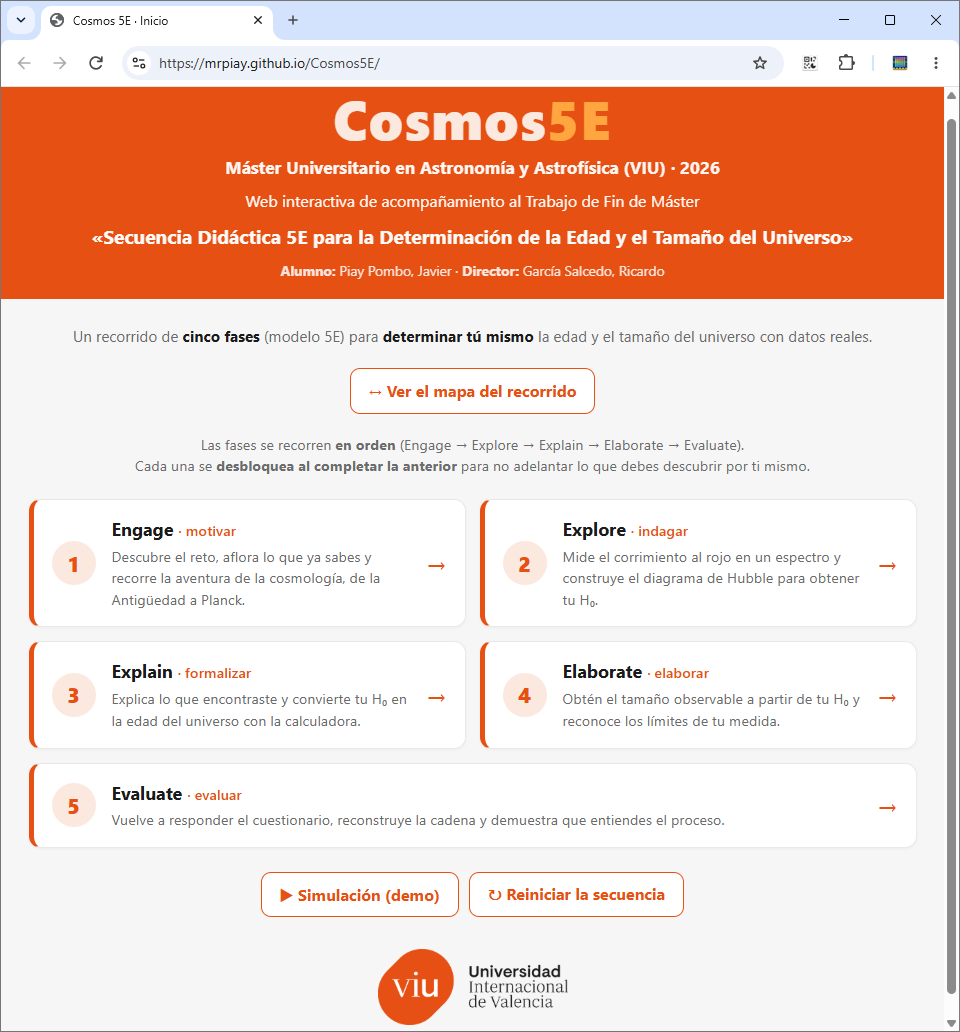
\includegraphics[width=0.85\textwidth]{./Images/web_v2_0_index.png}
\caption{Captura de la página de inicio de la web interactiva.}\label{fig:web-index}
\end{figure}

\subsection{Fundamento}

La web interactiva se fundamenta en la \textbf{revisión bibliográfica del Capítulo 2} ---de la que proceden los contenidos viables en el aula, las estrategias didácticas más eficaces y las ideas erróneas que conviene confrontar--- y emplea \textbf{datos y herramientas de acceso público}, citados a sus repositorios: las distancias del diagrama de Hubble proceden de la base de distancias independientes del corrimiento al rojo de NED \parencite{steer2017}, con el \textit{HST Key Project} \parencite{freedman2001} como contraste histórico; la calculadora se inspira en la de \textcite{wright2006}, reescrita en clave didáctica; y los valores cosmológicos actuales de referencia proceden de \textcite{planck2020}. Tanto la secuencia como la web interactiva se \textbf{inspiran} en los materiales y actividades docentes de la asignatura de Cosmología del Máster Universitario en Astronomía y Astrofísica de la VIU, \textbf{aprovechados y adaptados} al nivel de 2º de Bachillerato.

La transposición a este nivel implica sustituir lo inviable en el aula ---integrales de distancia cosmológica o software astronómico especializado no disponible en el aula--- por versiones interactivas, simplificadas y autónomas, centradas en el \textbf{régimen lineal} de la ley de Hubble ($v = H_{0}d$) y en la aproximación $t \approx 1/H_{0}$.

\subsection{Componentes}

La herramienta integra, para cada fase, cuatro tipos de componente:

\begin{itemize}
\item \textbf{Contenidos teóricos} breves y accesibles por concepto (escalas de espacio y tiempo, corrimiento al rojo, ley de Hubble-Lemaître, constante de Hubble, edad y tamaño del universo observable, ideas erróneas nucleares y naturaleza de la ciencia), acompañados de un \textbf{glosario} enlazado desde las actividades.
\item Una \textbf{calculadora didáctica} de $H_{0}$, la edad y el tamaño, concebida como una de las \textbf{herramientas clave} del conjunto: despliega la cadena de razonamiento paso a paso, explica cada término y \textbf{por qué interviene}, y hace visible la conversión de unidades que suele quedar oculta.
\item Un \textbf{diagrama de Hubble interactivo}, la otra herramienta clave: a partir de un conjunto de galaxias reales con su distancia y su velocidad de recesión, el alumnado ajusta una recta sobre los puntos representados y obtiene \textbf{su propio valor de $H_{0}$}. Las distancias proceden de métodos \textbf{independientes del corrimiento al rojo}, de modo que la ley de Hubble se «descubre» de forma genuina y no circular.
\item \textbf{La cadena de la medida}, una \textbf{secuencia de conceptos} visible en cada página de medida ---de Explore a Evaluate--- ($z \rightarrow v \rightarrow H_{0} \rightarrow$ edad $\rightarrow$ tamaño) que marca en qué punto del razonamiento se encuentra el alumnado y cómo cada concepto \textbf{conduce al siguiente} hasta comprender el valor final; no acumula números, sino que \textbf{encadena las ideas} del proceso.
\item Un \textbf{mapa del recorrido} accesible desde el inicio (Figura~\ref{fig:web-mapa}), que presenta el \textbf{propósito} y las \textbf{acciones} de cada fase y la pregunta que la enlaza con la siguiente ---una vista de conjunto para orientar al alumnado, sin adelantar las respuestas---.
\end{itemize}

\begin{figure}[htbp]
\centering
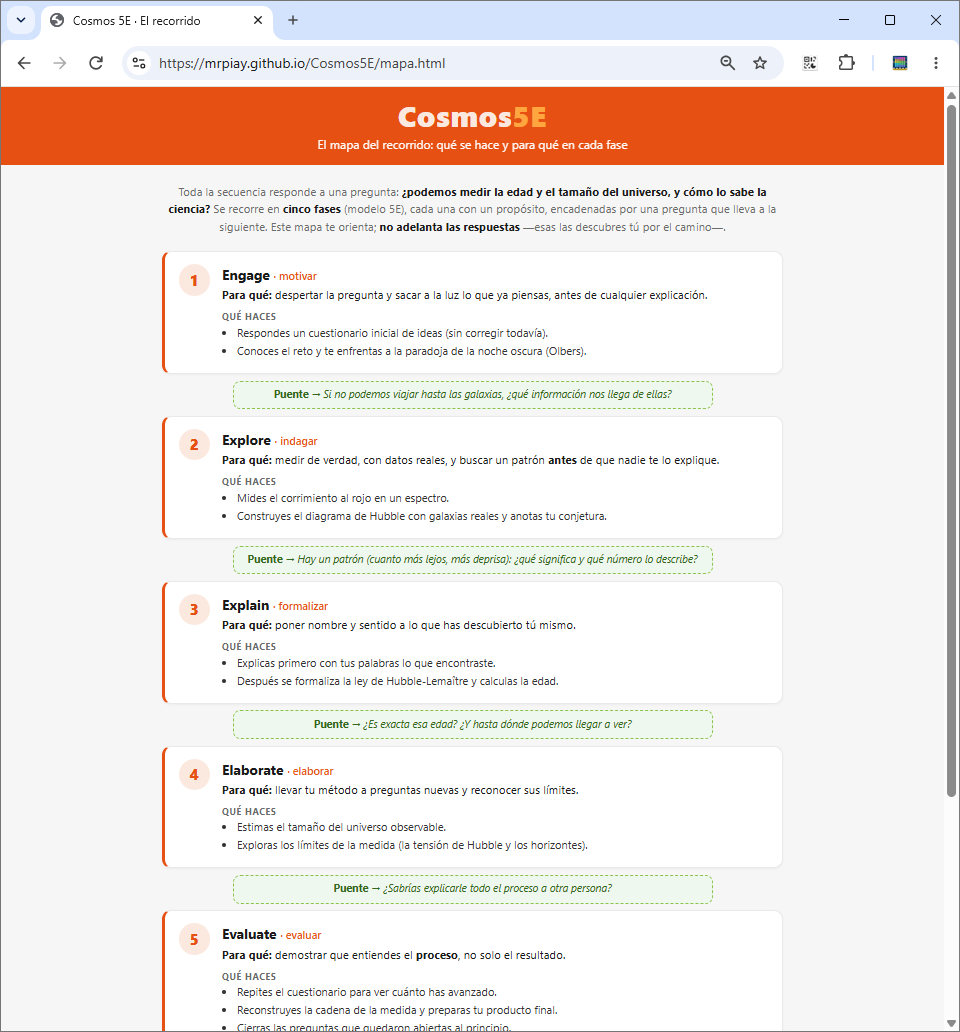
\includegraphics[width=0.85\textwidth]{./Images/web_v2_8_mapa.png}
\caption{Captura del \textbf{mapa del recorrido} de la secuencia 5E, accesible desde la página de inicio.}\label{fig:web-mapa}
\end{figure}

A ellos se suman los \textbf{instrumentos de evaluación} (cuestionario pre/post y rúbrica), descritos en §4.3.

\subsection{Principios de diseño}

La propuesta se rige por cuatro principios. \textbf{Autonomía y funcionamiento sin conexión}: construida con tecnologías web estándar, sin servidor ni dependencias externas, se abre en cualquier navegador sin instalación. \textbf{Adecuación al nivel}: vocabulario de 2º de Bachillerato y explicaciones antes que formalismo, con los valores actuales (Planck) como referencia pero dando prioridad al $H_{0}$ que \textbf{el propio alumnado mide}. \textbf{Equidad}: se mantiene una \textbf{alternativa no digital} (banda elástica y datos en papel) para quien no disponga de dispositivo. \textbf{Preguntar antes que explicar}: las cuestiones que Engage deja abiertas (los términos clave y la paradoja de Olbers) se mantienen vivas con \textbf{recordatorios} en cada fase ---«ya deberías poder responder\ldots»--- y se \textbf{cierran al final}, en Evaluate, cuando el alumnado ya tiene todas las piezas.

\subsection{Articulación con las cinco fases}

La herramienta se organiza como un recorrido por las cinco fases 5E; cada una integra su teoría, su actividad interactiva y su lugar en la cadena de la medida. La Tabla~\ref{tab:appfases} resume el encaje.

\begin{table}[ht]
\centering
\caption{Aportación de la herramienta en cada fase de la secuencia.}\label{tab:appfases}
\begin{tabularx}{\textwidth}{|>{\raggedright\arraybackslash}p{2.4cm}|>{\raggedright\arraybackslash}X|}
\hline
\rowcolor{naranja}
{\color{white}\textbf{Fase}} & {\color{white}\textbf{Aportación de la herramienta}} \\ \hline
Engage & Aflora las ideas previas con un \textbf{cuestionario conceptual} (sin adelantar respuestas); plantea el reto, define los términos clave, recorre la historia de la cosmología y provoca con la paradoja de Olbers. \\ \hline
Explore & En dos partes: medida del corrimiento al rojo en un espectro y \textbf{diagrama de Hubble interactivo} con galaxias reales, del que se obtiene el valor de $H_{0}$ (la pendiente). El alumnado \textbf{registra su conjetura} sobre lo observado, sin interpretarla todavía. \\ \hline
Explain & \textbf{Primero el alumnado explica} lo que encontró; después se formaliza la ley de Hubble-Lemaître y, con la \textbf{calculadora didáctica}, se obtiene la edad (cadena y conversión de unidades), con «rebobinar la expansión», el corrimiento cosmológico y el «calendario cósmico». \\ \hline
Elaborate & En dos partes: (1) el \textbf{tamaño} del universo observable ---radio de Hubble y por qué el observable real es mayor ($\sim$46\,000 millones de al)--- y una actividad de \textbf{transferencia} a otros valores de $H_{0}$; (2) los \textbf{límites} de la medida: tensión de Hubble, modelo $\Lambda$CDM y horizontes. \\ \hline
Evaluate & Cuestionario \textbf{post} (el mismo instrumento conceptual que el pre), repaso de la cadena ($z \rightarrow H_{0} \rightarrow$ edad $\rightarrow$ tamaño), \textbf{cierre de las preguntas abiertas del principio} (Olbers, edad, tamaño\ldots), lectura interactiva de las ecuaciones (clasificación por tipo) y guion del \textbf{producto final} con su rúbrica. \\ \hline
\end{tabularx}
\end{table}

\section{Desarrollo de las actividades por fase}\label{sec:desarrollo-detallado}

Esta sección desarrolla cada fase de la secuencia siguiendo la \textbf{plantilla común} definida en el Capítulo 3 (§3.7). El \textbf{diseño pedagógico} de cada fase ---el porqué de su función, la secuencia de actividades y las ecuaciones que introduce--- se ha detallado ya en el \textbf{recorrido por fases} de §\ref{sec:recorrido-fases}; para no duplicarlo, aquí cada ficha se centra en la \textbf{implementación en la web interactiva} y en los elementos operativos (contenido teórico al nivel del alumnado, interacción concreta, materiales, producto e indicadores de logro), remitiendo a aquel apartado para el desarrollo paso a paso. Todo ello se orienta a los objetivos de aprendizaje (OA1--OA7) y confronta las ideas erróneas de §3.5. Los materiales resultantes se recopilan en §4.6, y su versión completa constituye el guion de la web interactiva.

\subsection{Engage (motivar y aflorar ideas previas)}

\textbf{Pregunta que la abre:} ¿Tiene edad el universo? ¿Se puede determinar algo tan grande y lejano sin salir del aula?

\textbf{Objetivo(s) y OA:} despertar la pregunta motriz y aflorar las intuiciones sobre el espacio y el tiempo, diagnosticando concepciones \textit{(base para todos los OA; prepara OA1)}.

\textbf{Duración y agrupamiento:} 1 sesión (45 min); gran grupo con trabajo en pequeños grupos.

\subsubsection*{Qué sabemos e ideas previas}

Mediante un \textbf{cuestionario conceptual}, el alumnado responde, para cada concepto clave de la secuencia (año-luz, corrimiento al rojo, expansión, ley de Hubble, universo observable, etc.), una pregunta de opción múltiple ---con la opción \emph{«No lo sé / no lo tengo claro»} para quien no lo tenga claro, de modo que el pre-test queda completo---, \textbf{sin corrección a la vista} para no adelantar nada. Funciona a la vez como sondeo de \textbf{ideas previas} y como \textbf{pre-test conceptual}, el mismo instrumento que se repite en Evaluate.

\subsubsection*{Contenido teórico}

\textit{Nivel cualitativo, sin fórmulas.}
\begin{itemize}
\item \textbf{Qué significa determinar la edad y el tamaño:} la \textbf{edad} es el tiempo transcurrido desde el Big Bang ($\sim$13\,800 millones de años), no la de un astro concreto; el \textbf{tamaño} es el del universo \textbf{observable} ---la región cuya luz nos ha dado tiempo a alcanzar---, no el del universo total, que podría ser infinito.
\item \textbf{Medir sin viajar:} no vamos a las galaxias; leemos su \textbf{luz}, que transporta la información. Y como la luz tarda en llegar, \textbf{mirar lejos es mirar al pasado} (la luz como «máquina del tiempo»).
\item \textbf{La enormidad del tiempo cósmico, como pregunta abierta:} el universo es antiquísimo; ¿qué ha ocurrido en todo ese tiempo y cuándo? La pregunta se \textbf{planta aquí} y se responde en Explain (con el «calendario cósmico»).
\item \textbf{La cosmología como aventura (naturaleza de la ciencia):} nuestra visión del universo ha \textbf{cambiado} ---de la Tierra en el centro a la edad medida por el satélite Planck--- y cada salto llegó con una \textbf{tecnología} nueva para captar más luz.
\item \textbf{Paradoja de Olbers:} en un universo infinito, eterno y estático, \textbf{toda línea de visión} acabaría en la superficie de una estrella ---la debilidad de las lejanas se compensa con su mayor número--- y el cielo nocturno debería \textbf{brillar como el Sol}. Como no lo hace, alguna de esas premisas debe fallar: se plantea como \textbf{interrogante abierto} (¿cuál?), \textbf{sin resolver todavía} ---el alumnado lo retomará y cerrará al final---. La noche oscura es, así, un gancho hacia un universo \textbf{con historia}.
\end{itemize}

\subsubsection*{Desarrollo de la actividad}

El desarrollo paso a paso de esta fase ---reto y pregunta motriz, cuestionario conceptual (pre-test), definición de términos clave, aventura de la cosmología y paradoja de Olbers--- se detalla en el diseño de la secuencia (§\ref{sec:engage}). La paradoja de Olbers se plantea como provocación cualitativa \parencite{santos2014}, con apoyo opcional en la narrativa histórica \textit{Cosmic Times} \parencite{lochner2009,nunes2025}. Su implementación en la web se recoge a continuación.

\subsubsection*{Interacción en la web}

\begin{itemize}
\item \textbf{«El reto»:} una entrada que fija qué se va a determinar, por qué y para qué, con la pregunta motriz.
\item \textbf{Cuestionario conceptual:} por cada concepto, una \textbf{pregunta de opción múltiple} con distractores basados en ideas erróneas y una opción \emph{«No lo sé / no lo tengo claro»}; sin corrección, es el pre-test conceptual que se recupera y repite en Evaluate.
\item \textbf{Tarjetas de términos:} al pulsar cada término (edad, tamaño, universo observable, medir sin viajar) se revela «lo que suele creerse» frente a una \textbf{pista que despierta la curiosidad} ---una pregunta o una analogía que remite a fases posteriores---, no la definición completa.
\item \textbf{Línea de tiempo interactiva:} hitos de la historia de la cosmología (de la Antigüedad a Planck); al pulsar cada uno se revela qué cambió y la \textbf{tecnología} que lo permitió; los más recientes (expansión, fondo de microondas, edad) se plantean como \textbf{interrogantes} para no adelantar respuestas.
\item \textbf{Olbers interactivo:} un \textbf{control deslizante} que va llenando el cielo de estrellas (del mismo color) hasta \textbf{cubrirlo por completo}, mostrando que el fulgor surge de \textbf{tapar todos los huecos} y no de que cada estrella brille más; un \textbf{desplegable} aclara el porqué (el \textbf{brillo de superficie} no decae con la distancia). Se plantea como \textbf{interrogante} ---¿qué premisa falla?---, \textbf{sin resolverlo aquí}: la respuesta se construye a lo largo de la secuencia y se cierra en Evaluate.
\end{itemize}

\subsubsection*{Idea errónea que confronta}

Universo estático o eterno; Big Bang como «explosión»; dificultad para manejar las escalas espaciales y temporales.

\subsubsection*{Espacio--tiempo que se trabaja}

Primeras intuiciones; la enormidad del tiempo cósmico (planteada como pregunta abierta); la luz como puente entre distancia y tiempo ---mirar lejos es mirar al pasado---.

\subsubsection*{Materiales}

\begin{itemize}
\item \textbf{Hitos de la línea de tiempo} de la cosmología, con su tecnología asociada.
\item \textbf{Simulación interactiva de la paradoja de Olbers} (control local de «cobertura del cielo»).
\item \textbf{Cuestionario conceptual} de 15 ítems de opción múltiple (pre-test = post-test), con distractores basados en las ideas erróneas (§\ref{sec:instrumentos}).
\end{itemize}

\subsubsection*{Producto de la fase}

Primeras hipótesis sobre la edad y el tamaño del universo, y una idea clara de qué significan esos términos y de cómo la ciencia ha llegado a medirlos.

\subsubsection*{Indicadores de logro}

\begin{itemize}
\item Distingue qué significan la \textbf{edad} y el \textbf{tamaño} (observable) del universo, y reconoce que ese conocimiento ha \textbf{evolucionado} con la ciencia y la tecnología.
\item Expresa una hipótesis razonada sobre si el universo tiene edad y cómo podría determinarse.
\item Deja constancia de sus ideas previas (pre-test) para contrastarlas en Evaluate.
\end{itemize}

\subsubsection*{Puente a la siguiente fase}

Si no podemos ir hasta allí, ¿qué información nos llega de las galaxias? $\rightarrow$ \textbf{la luz}. Y queda rondando una \textbf{pregunta} ---¿qué ocurrió desde el Big Bang hasta hoy?--- que se responderá en Explain (con el «calendario cósmico»).

\begin{figure}[htbp]
\centering
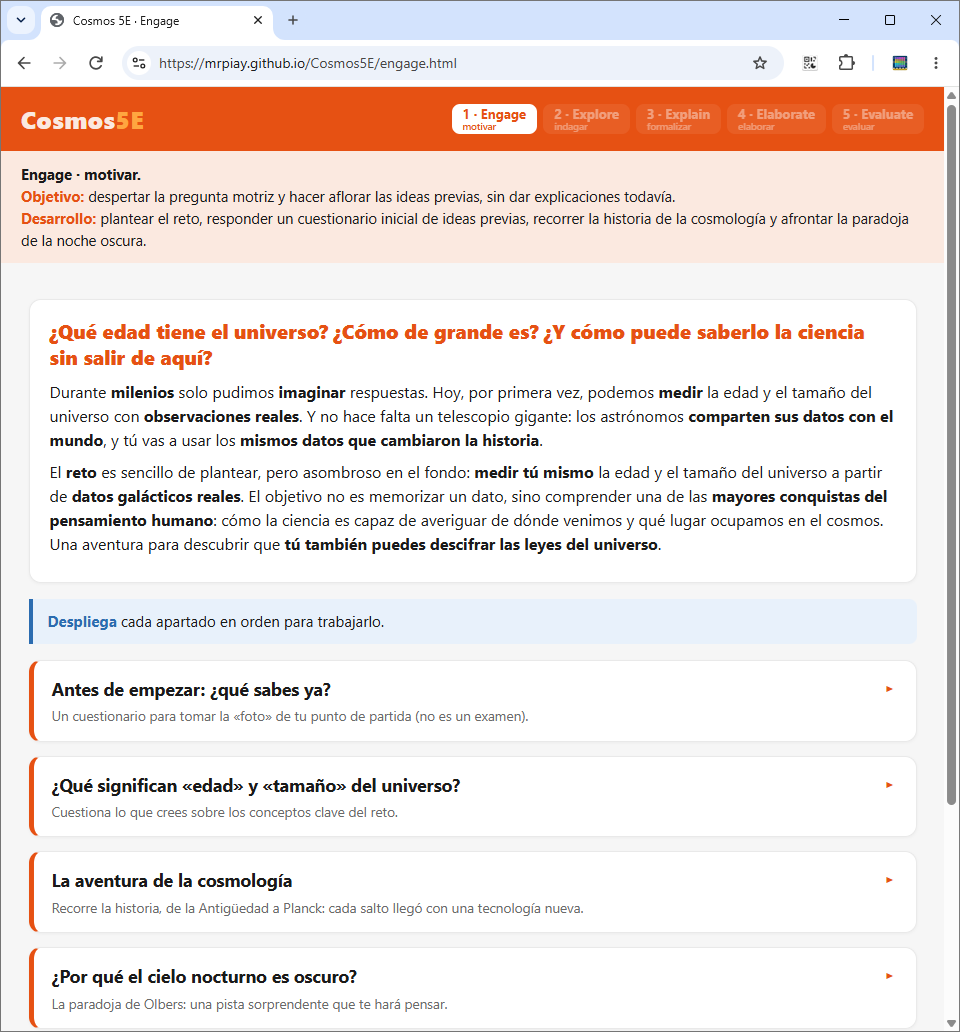
\includegraphics[width=0.82\textwidth]{./Images/web_v2_1_engage.png}
\caption{Captura de la sección \textbf{Engage} en la web interactiva.}\label{fig:web-engage}
\end{figure}

\subsection{Explore (indagación con datos)}

\textbf{Pregunta que la abre:} ¿Qué nos dice la luz de las galaxias? ¿Se mueven?

\textbf{Objetivo(s) y OA:} obtener $H_{0}$ a partir de la medida de la distancia y de la recesión \textit{(OA1, OA2, OA3)}.

\textbf{Duración y agrupamiento:} 2 sesiones (45 min); parejas o pequeños grupos.

\subsubsection*{Qué sabemos e ideas previas}

Concepto de \textbf{onda} y \textbf{efecto Doppler} (del sonido), qué es un \textbf{espectro}, la relación velocidad = distancia/tiempo y el \textbf{ajuste de una recta}.

\subsubsection*{Contenido teórico}

\begin{itemize}
\item \textbf{Cómo se miden las distancias} astronómicas (paralaje y candelas estándar), en breve, para que no sean «magia»; el \textbf{año-luz} como unidad del espacio.
\item \textbf{Corrimiento al rojo:} la luz de las galaxias llega «estirada» hacia el rojo; se mide con $z = \Delta\lambda/\lambda$ (desplazamiento relativo de una línea del espectro respecto a su longitud de onda en reposo).
\item \textbf{Velocidad de recesión:} para galaxias cercanas ($z$ pequeño), $v \approx c\,z$ \textit{(la web avisa de que esto solo vale a $z$ pequeño)}.
\item \textbf{El patrón velocidad--distancia:} al representar $v$ frente a $d$, los puntos se alinean formando una recta cuya \textbf{pendiente} es la medida que se busca (se la llamará $H_{0}$). En Explore \textbf{no se nombra aún la ley ni se interpreta el patrón} ---qué significa o por qué la recta pasa por el origen---: eso se reserva para Explain.
\end{itemize}

\subsubsection*{Desarrollo de la actividad}

El desarrollo paso a paso de las dos actividades de esta fase ---medir el corrimiento al rojo ($z = \Delta\lambda/\lambda$, $v = c\,z$) y descubrir la relación distancia--velocidad construyendo el diagrama de Hubble y registrando la conjetura--- se detalla en el diseño de la secuencia (§\ref{sec:explore}). En el aula puede apoyarse con banda elástica y \textit{Tracker} \parencite{suarez2025} o con datos reales en hoja de cálculo \parencite{cardona2016,hyde2021}. Su implementación en la web se recoge a continuación.

\subsubsection*{Interacción en la web}

\begin{itemize}
\item \textbf{Explorar el corrimiento al rojo:} sobre una \textbf{galaxia hipotética}, el alumnado \textbf{arrastra} la línea de emisión (H$\alpha$) y ve \textbf{en vivo} cómo su desplazamiento se traduce en $z = \Delta\lambda/\lambda$ y $v = c\,z$; se plantea como \textbf{pregunta abierta} si de verdad es un efecto Doppler ---se resolverá en Explain---.
\item \textbf{Diagrama de Hubble interactivo (la actividad central):} el alumnado ajusta la recta sobre los puntos ya representados (arrastrando su pendiente o con «ajuste automático»); la web muestra su valor ---la pendiente--- y las barras de error de los puntos dejan ver la incertidumbre de los datos. Ese es el valor que llevará a Explain, \textbf{todavía sin interpretar} qué significa.
\item \textbf{Registro de la conjetura:} al terminar, un formulario recoge qué patrón ve el alumnado, qué cree que significa la pendiente, por qué algunas galaxias se salen y qué ocurriría al «rebobinar» el tiempo; hay que completarlo para poder continuar, y se recupera en Explain.
\item \textbf{Datos de partida:} 15 galaxias reales de 15 a 153 Mpc con distancia independiente del corrimiento al rojo y velocidad $v = c\,z$; el ajuste con las de flujo limpio ($v > 3000$ km/s) da $H_{0} \approx 70$ y, por tanto, $1/H_{0} \approx 14$ Gyr. Se incluyen a propósito galaxias cercanas dispersas (NGC 4536, NGC 4639\ldots) para discutir las velocidades peculiares. Fuente: NED-D \parencite{steer2017}, con el \textit{HST Key Project} \parencite{freedman2001} como contraste.
\item \textbf{Alternativa no digital} (§4.4): la misma actividad con banda elástica y datos en papel.
\end{itemize}

\subsubsection*{Idea errónea que confronta}

«Todo corrimiento al rojo es efecto Doppler ordinario»; «la expansión es el movimiento propio de las galaxias por el espacio».

\subsubsection*{Espacio--tiempo que se trabaja}

La medida del \textbf{espacio}: distancias astronómicas y el año-luz.

\subsubsection*{Materiales}

\begin{itemize}
\item \textbf{Espectro(s)} de trabajo: espectro de una galaxia (real o representativa) con una línea identificable ---p.\,ej. H$\alpha$--- para medir su corrimiento al rojo $z$.
\item \textbf{Dataset del diagrama de Hubble:} 15 galaxias (NED-D) con distancia, velocidad $v = c\,z$ e incertidumbre.
\item Herramienta de \textbf{ajuste de recta} (web) y su alternativa con \textbf{banda elástica} (no digital).
\end{itemize}

\subsubsection*{Producto de la fase}

El diagrama de Hubble del alumnado y su valor de $H_{0}$ (con incertidumbre).

\subsubsection*{Indicadores de logro}

\begin{itemize}
\item Mide $z$ correctamente a partir de un espectro y obtiene $v = c\,z$.
\item Construye el diagrama de Hubble y obtiene un $H_{0}$ razonable, con noción de incertidumbre.
\item Distingue la recesión por expansión del espacio del movimiento propio de la galaxia.
\end{itemize}

\subsubsection*{Puente a la siguiente fase}

Hay un patrón ($v$ crece con $d$): ¿qué significa y qué número lo describe? $\rightarrow$ la constante de Hubble y qué podemos calcular con ella.

\begin{figure}[htbp]
\centering
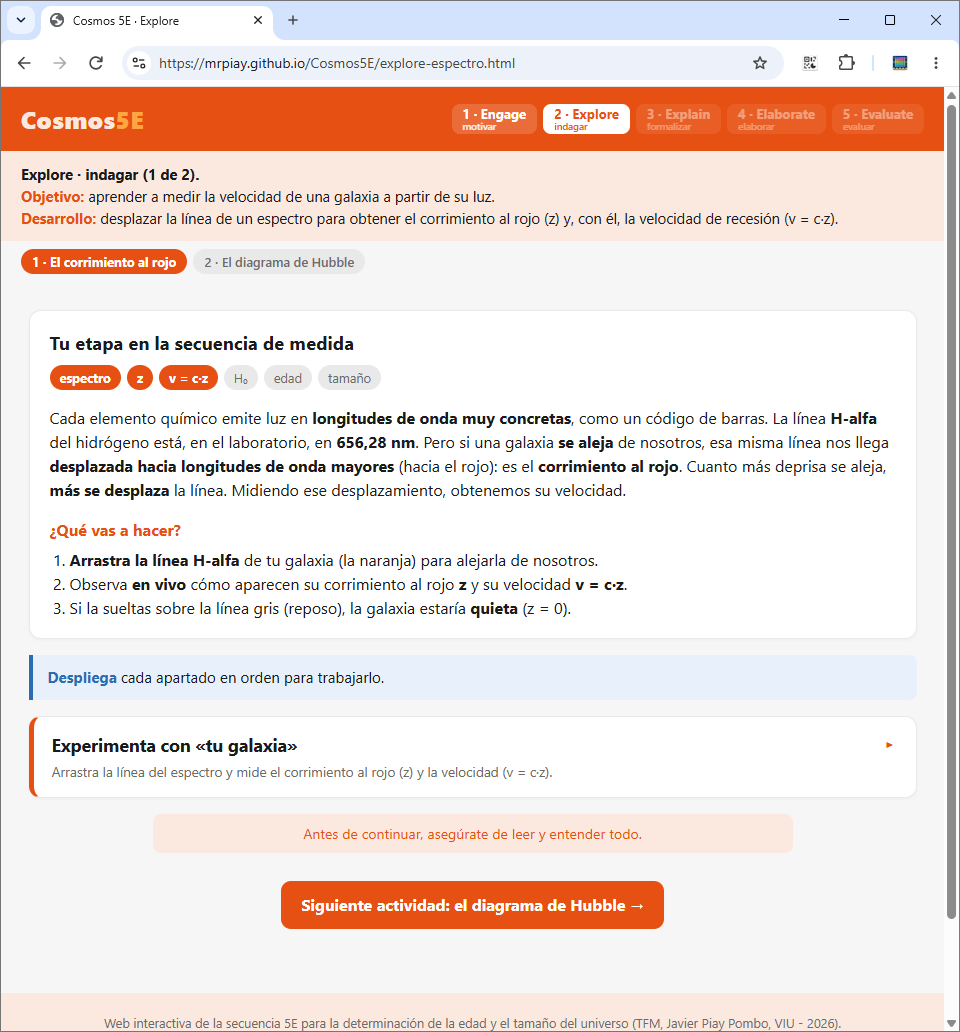
\includegraphics[width=0.48\textwidth]{./Images/web_v2_2_espectro.png}\hfill
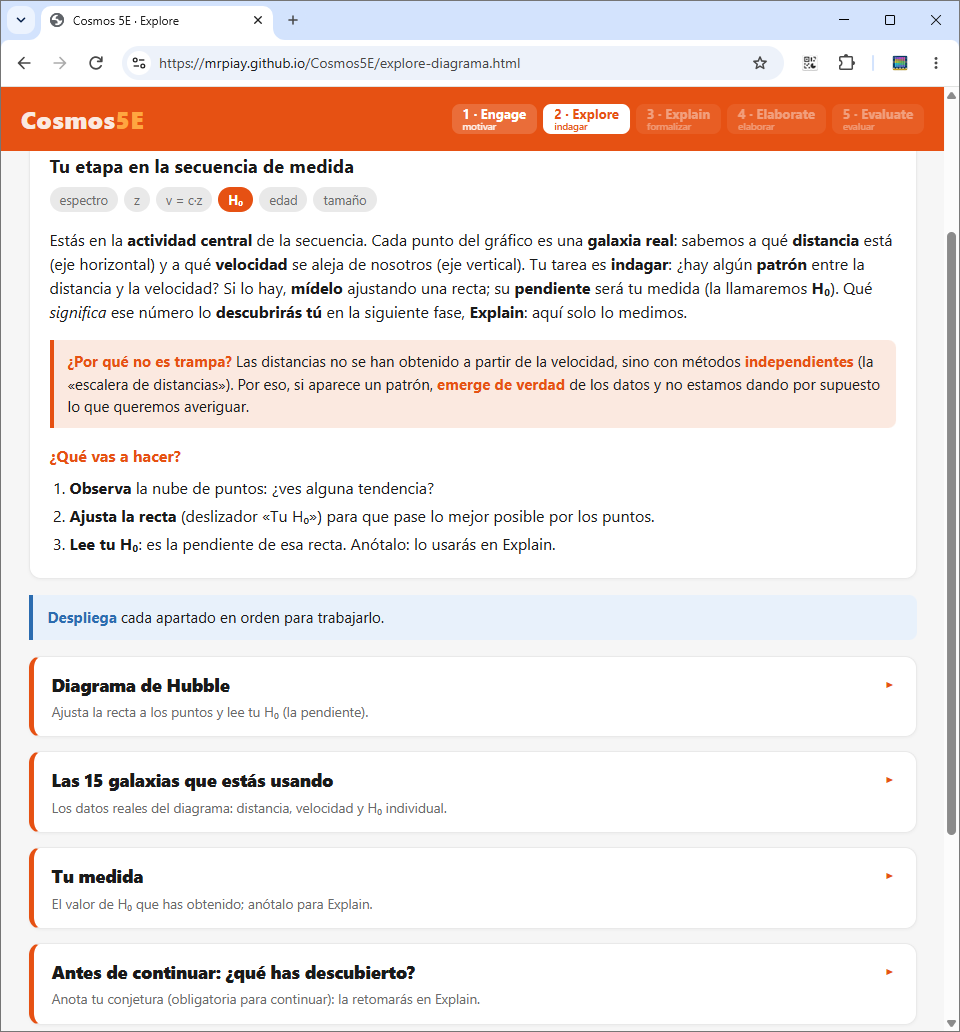
\includegraphics[width=0.48\textwidth]{./Images/web_v2_3_diagrama.png}
\caption{Capturas de la sección \textbf{Explore} en la web interactiva: espectro (izquierda) y diagrama de Hubble (derecha).}\label{fig:web-explore}
\end{figure}

\subsection{Explain (formalizar el concepto)}

\textbf{Pregunta que la abre:} ¿Qué significa que la velocidad aumente con la distancia? ¿Qué es $H_{0}$ y qué podemos calcular con él?

\textbf{Objetivo(s) y OA:} conectar $H_{0}$ con la edad del universo, situarla en perspectiva y formalizar el corrimiento al rojo \textit{(OA2, OA3, OA4)}.

\textbf{Duración y agrupamiento:} 1 sesión (45 min); gran grupo con resolución individual.

\subsubsection*{Qué sabemos e ideas previas}

El \textbf{valor} (la pendiente) y la \textbf{recta $v$--$d$} que el propio alumnado obtuvo en Explore, y la \textbf{conjetura} que anotó allí.

\subsubsection*{Contenido teórico}

\begin{itemize}
\item \textbf{Qué es $H_{0}$ de verdad:} el \textbf{ritmo de expansión} del universo (cuánta velocidad de recesión por cada unidad de distancia); unidades km/s/Mpc.
\item \textbf{De $H_{0}$ a la edad:} por \textbf{extrapolación lineal} de la tasa de expansión actual, el tiempo transcurrido desde el Big Bang sería $t \approx 1/H_{0}$ (\textbf{tiempo de Hubble}), un valor del \textbf{orden} de la edad.
\item \textbf{Conversión de unidades} (explícita y central): con $1\ \text{Mpc} = 3{,}086\cdot10^{19}$ km, $1/H_{0} \approx 4{,}4\cdot10^{17}$ s $\approx 14\,000$ millones de años (la web lo muestra paso a paso).
\item \textbf{Por qué $1/H_{0}$ es la edad del universo:} al \textbf{rebobinar} la expansión, las \textbf{distancias entre todas las galaxias se reducen a la vez} ---las lejanas van proporcionalmente más rápido---, hace $\sim 1/H_{0}$, hasta un estado inicial muy denso y caliente (el Big Bang), \textbf{sin un punto ni un centro privilegiado}. Es una \textbf{distancia $\div$ velocidad de recesión} ($d/v$) ---la edad del \textbf{universo entero}---, y no el tiempo que tardó en llegarnos la luz de una galaxia ($d/c$, mucho menor).
\item \textbf{El corrimiento al rojo de la luz es siempre cosmológico:} la luz llega estirada porque \textbf{el espacio se estira} mientras viaja, no porque la galaxia «vuele» a través de él. En galaxias cercanas ($z$ pequeño), la \textbf{fórmula del Doppler} $v = c\,z$ da el número correcto y se usa como \textbf{atajo}, pero \textbf{cualitativamente es incorrecta}; solo el pequeño movimiento propio (velocidades peculiares) es un Doppler real \parencite{xu2018,possel2020,marshall2022}.
\item \textbf{La edad, en perspectiva (calendario cósmico):} esos $\sim$14\,000 millones de años son inabarcables; comprimir toda la historia del universo en un año hace tangible la escala ---la humanidad ocupa los últimos segundos--- y responde a la \textbf{gran pregunta} planteada en Engage \parencite{colantonio2019}.
\end{itemize}

\subsubsection*{Desarrollo de la actividad}

El desarrollo paso a paso de esta fase ---recuperar y poner en común la explicación del alumnado; formalizar $v = H_{0}d$ e identificar la pendiente como $H_{0}$; deducir y calcular $t \approx 1/H_{0}$ con la conversión de unidades; recorrer la historia de la expansión (hacia adelante y atrás); distinguir el corrimiento al rojo cosmológico del Doppler; y poner la edad en perspectiva con el calendario cósmico--- se detalla en el diseño de la secuencia (§\ref{sec:explain}). Su implementación en la web se recoge a continuación.

\subsubsection*{Interacción en la web}

\begin{itemize}
\item \textbf{«Tu explicación» (antes de nada):} la web recupera la conjetura de Explore y pide al alumnado que explique con sus palabras lo que encontró; \textbf{hay que guardarla para poder revelar la explicación científica}, de modo que se razona primero y la formalización llega después.
\item \textbf{Calculadora didáctica (la herramienta central de esta fase):} el alumnado introduce su $H_{0}$ (el de Explore) y ve salir la edad, con la cadena y la conversión de unidades a la vista, término a término.
\item \textbf{«La historia del universo» (interactivo):} un deslizador recorre la historia ---hacia adelante y hacia atrás--- sobre un \textbf{trozo de espacio} representado como una textura que cambia de escala: al rebobinar, el espacio se \textbf{comprime por igual en todas partes} (sin un centro) hasta un estado \textbf{denso y caliente} anterior a las galaxias; al avanzar, se forman las galaxias y, más tarde, aparecemos \textbf{nosotros} (la Tierra, un «punto azul pálido»), que las vemos ya muy lejos. Hace tangible que $1/H_{0}$ marca el \textbf{orden} de la edad y que las estructuras ---y nosotros--- se formaron mucho después del inicio.
\item \textbf{«El corrimiento al rojo de la luz»:} explica que el estiramiento es \textbf{siempre cosmológico} y que $v = c\,z$ es solo un \textbf{atajo} numérico válido en galaxias cercanas ($z$ pequeño), cualitativamente incorrecto; lo distingue de las velocidades peculiares (Doppler real) y recuerda que los \textbf{sistemas ligados} (galaxias, Sistema Solar, personas) no se expanden.
\item \textbf{«Calendario cósmico» (cierre):} tras estimar la edad, un deslizador comprime toda la historia del universo en un año y muestra cuándo ocurre cada suceso ---la humanidad, en los últimos segundos---; \textbf{responde la gran pregunta} planteada en Engage.
\end{itemize}

\subsubsection*{Idea errónea que confronta}

Corrimiento al rojo = Doppler; los sistemas ligados (galaxias, Sistema Solar, personas) se expanden.

\subsubsection*{Espacio--tiempo que se trabaja}

La \textbf{unión de ambos}: de una velocidad y una distancia se obtiene un tiempo (la edad); mirar lejos es mirar al pasado. La escala de esa edad se hace tangible con el \textbf{calendario cósmico}.

\subsubsection*{Materiales}

\begin{itemize}
\item \textbf{Calculadora didáctica} (web).
\item Gráfico interactivo \textbf{«rebobinar la expansión»} (web).
\item Recurso \textbf{«el corrimiento al rojo de la luz»} (web): $v = c\,z$ como atajo frente al estiramiento cosmológico.
\item \textbf{Datos del calendario cósmico} (sucesos y su fecha en el «año» del universo).
\end{itemize}

\subsubsection*{Producto de la fase}

Estimación razonada de la edad del universo (a partir de su $H_{0}$), con la conversión de unidades hecha.

\subsubsection*{Indicadores de logro}

\begin{itemize}
\item Interpreta $H_{0}$ como ritmo de expansión (no como una velocidad sin más).
\item Deduce y calcula $t \approx 1/H_{0}$ con la conversión de unidades correcta.
\item Explica que el corrimiento al rojo cosmológico es estiramiento del espacio y que los sistemas ligados no se expanden.
\item Explica por qué $1/H_{0}$ es la edad del universo ($d/v$) y no el tiempo de viaje de la luz de un objeto ($d/c$).
\item Sitúa la edad estimada en perspectiva con el calendario cósmico.
\end{itemize}

\subsubsection*{Puente a la siguiente fase}

¿Es exacta esa edad? ¿Y hasta dónde podemos ver? $\rightarrow$ los límites de la estimación y el tamaño del universo observable.

\begin{figure}[htbp]
\centering
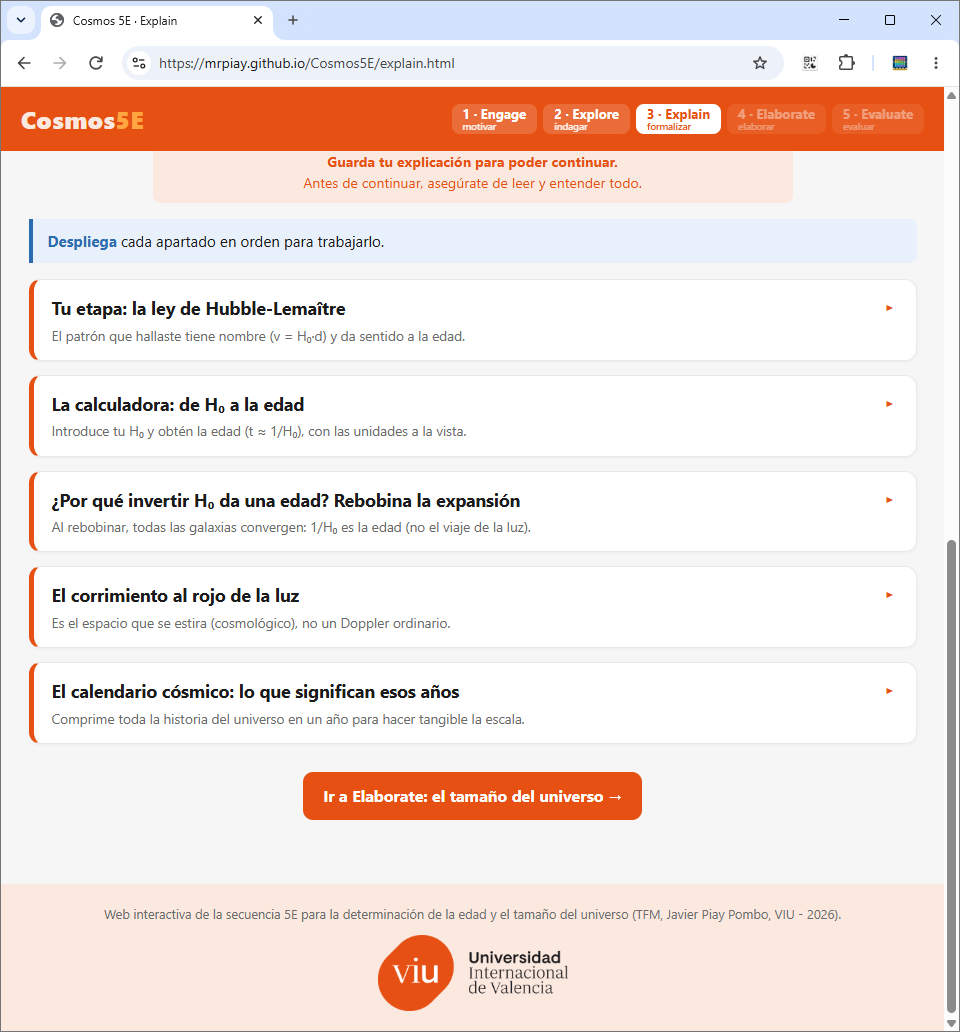
\includegraphics[width=0.82\textwidth]{./Images/web_v2_4_explain.png}
\caption{Captura de la sección \textbf{Explain} en la web interactiva.}\label{fig:web-explain}
\end{figure}

\subsection{Elaborate (refinar y contextualizar la medida)}

\textbf{Pregunta que la abre:} ¿Qué tamaño tiene lo observable y qué límites tiene nuestra estimación?

\textbf{Objetivo(s) y OA:} refinar la medida y reconocer sus límites (calcular el \textbf{tamaño} del universo observable y entender por qué $t \approx 1/H_{0}$ es solo una primera aproximación) y valorar que la ciencia avanza discutiendo modelos y teorías \textit{(OA4, OA5, OA6, OA7)}.

\textbf{Duración y agrupamiento:} 2 sesiones (45 min c/u); pequeños grupos con debate en gran grupo. La \textbf{primera} se centra en el \textbf{tamaño observable} (radio de Hubble, su relación con el radio observable y la CMB); la \textbf{segunda}, en los \textbf{límites y matices} (alcance de $1/H_{0}$, horizonte de sucesos ---un paso más allá---, $\Lambda$CDM y tensión de Hubble).

\subsubsection*{Qué sabemos e ideas previas}

La \textbf{edad estimada} ($t \approx 1/H_{0}$) y el \textbf{valor de $H_{0}$} obtenidos en las fases anteriores.

\subsubsection*{Contenido teórico}

\begin{itemize}
\item \textbf{El radio de Hubble (escala característica de distancia):} $R \approx c\,(1/H_{0}) = c/H_{0}$ ($\approx 14\,000$ millones de años-luz con $H_{0} \approx 70$); \emph{no} es el tamaño del universo observable.
\item \textbf{Matiz (para no enseñar un error):} el radio observable real es mayor ($\sim$46\,000 millones de años-luz; el diámetro, $\sim$92\,000) porque el espacio se estiró mientras la luz viajaba; en bachillerato se estima solo el orden de magnitud, pues el cálculo exacto exige integrar la expansión (fuera del alcance) \parencite{linton2012}.
\item \textbf{El alcance de $t \approx 1/H_{0}$:} da una escala del \textbf{orden de la edad}; el valor \textbf{preciso} depende tanto del \textbf{valor de $H_{0}$} como de la \textbf{historia de la expansión} $H(t)$. Una fuente de incertidumbre muy debatida es el propio $H_{0}$ ---de ahí la tensión de Hubble---.
\item \textbf{El modelo estándar y la naturaleza de la ciencia:} el consenso actual, $\Lambda$CDM, describe un universo \textbf{plano} y de \textbf{unos 13\,800 millones de años}, dominado por la \textbf{energía oscura} ($\Lambda$, $\sim$68\,\%, que acelera la expansión) y la \textbf{materia oscura} (CDM, $\sim$27\,\%, que gravita), con solo un $\sim$5\,\% de materia ordinaria; encaja con observaciones independientes (fondo cósmico de microondas, supernovas y distribución de galaxias). No es un dogma: persiste la \textbf{tensión de Hubble} ---distintos métodos dan valores de $H_{0}$ algo distintos y, por tanto, edades algo distintas--- y hay teorías alternativas en la frontera (p.\,ej. MOND o la gravedad conforme) \parencite{planck2020}.
\item \textbf{Materia oscura $\neq$ energía oscura} (conceptos distintos: una «pesa», la otra «acelera»).
\item \textbf{El último horizonte (los límites de lo observable) ---un paso más allá---:} el universo observable \textbf{no crece sin límite} ---su radio tiende a un valor máximo---; más allá del \textbf{horizonte de sucesos cosmológico} ($\sim$16\,000 millones de años-luz) la expansión acelerada impide que la luz que las galaxias emiten \textbf{hoy} llegue jamás. Es un horizonte \textbf{distinto} de la esfera de Hubble ($\sim$14) y del universo observable ($\sim$46), y enlaza con la paradoja de Olbers de Engage.
\end{itemize}

\subsubsection*{Desarrollo de la actividad}

El desarrollo paso a paso de las dos partes de esta fase ---\textbf{el tamaño observable} (radio de Hubble $c/H_{0}$ y por qué el observable real es mayor) y \textbf{los límites de la medida} (transferencia a otros valores de $H_{0}$, tensión de Hubble y modelo estándar $\Lambda$CDM)--- se detalla en el diseño de la secuencia (§\ref{sec:elaborate}). La energía oscura aparece solo como \textbf{matiz} de la medida \parencite{hyde2021,pereira2019,raymundo2022}. Su implementación en la web se recoge a continuación.

\subsubsection*{Interacción en la web}

\begin{itemize}
\item \textbf{El tamaño observable, en dos pasos:} primero el \textbf{radio de Hubble} $R \approx c/H_{0}$ como \textbf{escala característica}; después, un \textbf{esquema interactivo} en el que se elige la \textbf{distancia de la fuente} (de una galaxia cercana al fondo de microondas) y, al avanzar el tiempo, el espacio se estira \textbf{en todas partes} (una rejilla) y la galaxia se aleja, con \textbf{cifras que se actualizan} ---camino recorrido, expansión, distancias y la \textbf{razón distancia hoy $\div$ camino}--- que hacen ver que la luz de las fuentes lejanas \textbf{al principio pierde terreno} y que esa razón \textbf{crece con la distancia} (de $\sim$1{,}2 en las cercanas a $\sim$3{,}3 en el borde): \textbf{no es una regla fija}, sino que proviene de la historia de la expansión. Así el \textbf{radio observable} ($\sim$46\,000 millones de años-luz; el diámetro, $\sim$92\,000) resulta \textbf{bastante mayor} que el radio de Hubble, aunque son \textbf{magnitudes distintas}. Se acompaña de una \textbf{derivación cualitativa con el fondo cósmico de microondas} (su $z \approx 1100$) que explica por qué el radio observable supera a $c \times$ edad.
\item \textbf{El modelo estándar $\Lambda$CDM en breve:} una ficha que resume qué contiene el universo ---con la distinción entre \textbf{materia oscura} («pesa», gravita) y \textbf{energía oscura} («acelera» la expansión)--- y que su expansión se \textbf{acelera}, como contexto de la medida.
\item \textbf{La tensión de Hubble:} se contrastan dos valores típicos ($\sim$67 de Planck y $\sim$73 de supernovas) y sus edades algo distintas, como ejemplo de incertidumbre y debate abierto (el efecto numérico de cambiar $H_{0}$ ya se explora en «Transferencia»).
\item \textbf{Sección de cierre «Un último horizonte» (un paso más allá):} distingue los \textbf{tres radios} ---esfera de Hubble ($\sim$14), horizonte de sucesos ($\sim$16) y universo observable ($\sim$46)--- y, con un \textbf{diagrama} y un \textbf{ejemplo numérico paso a paso} (un \textbf{modelo didáctico simplificado}, no una descripción exacta: el fotón avanza a $c$ y el espacio se expande un porcentaje fijo por paso), muestra por qué la luz que las galaxias más lejanas emiten \textbf{hoy} \textbf{nunca} nos alcanzará ---sin recurrir a velocidades superlumínicas--- y por qué el tamaño observable tiende a un techo; cierra retomando el «tercer factor» de la paradoja de Olbers.
\item \textbf{Transferencia:} el alumnado introduce otros valores de $H_{0}$ (Planck, supernovas, otro grupo) y compara al instante las edades y tamaños resultantes.
\end{itemize}

\subsubsection*{Idea errónea que confronta}

$t = 1/H_{0}$ como valor exacto; el radio observable como $c \times$ edad; energía oscura como sustancia o fuerza; confusión materia/energía oscura; la recesión superlumínica (creer que las galaxias «se alejan más rápido que la luz»); la ciencia como conjunto de hechos cerrados.

\subsubsection*{Espacio--tiempo que se trabaja}

El \textbf{tamaño} (espacio) del universo observable y los límites de la medida.

\subsubsection*{Materiales}

\begin{itemize}
\item \textbf{Calculadora didáctica} (paso «tamaño»), \textbf{deslizador} de la tensión de Hubble y \textbf{ficha del modelo $\Lambda$CDM}.
\item \textit{(Opcional)} datos de supernovas o simulador de energía oscura.
\end{itemize}

\subsubsection*{Producto de la fase}

Estimación refinada del tamaño observable y una explicación de los límites de la estimación.

\subsubsection*{Indicadores de logro}

\begin{itemize}
\item Calcula el tamaño observable (orden de magnitud) a partir de su $H_{0}$.
\item Reconoce que $1/H_{0}$ es una \textbf{estimación muy buena} de la edad (y que su valor depende del $H_{0}$ adoptado) y explica por qué el tamaño observable real es mayor que $c \times$ edad.
\item Distingue la materia oscura de la energía oscura.
\item Argumenta que la ciencia progresa debatiendo entre modelos (tensión de Hubble, alternativas, consenso $\Lambda$CDM).
\end{itemize}

\subsubsection*{Puente a la siguiente fase}

¿Sabríamos explicar todo el proceso a otra persona? $\rightarrow$ demostrar que entendemos el proceso, no solo el resultado.

\begin{figure}[htbp]
\centering
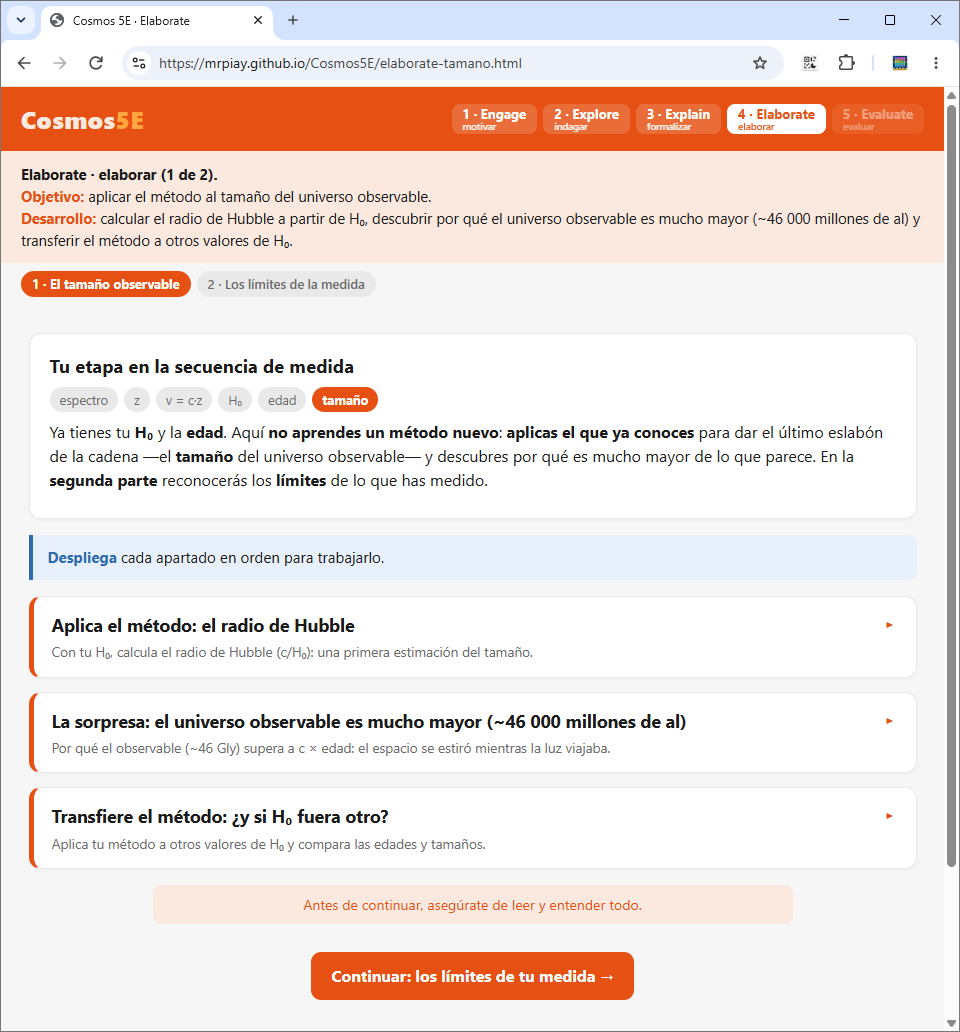
\includegraphics[width=0.82\textwidth]{./Images/web_v2_5_elaborate_tamano.png}
\caption{Captura de la sección \textbf{Elaborate}, parte 1: el tamaño del universo observable.}\label{fig:web-elaborate-tamano}
\end{figure}

\begin{figure}[htbp]
\centering
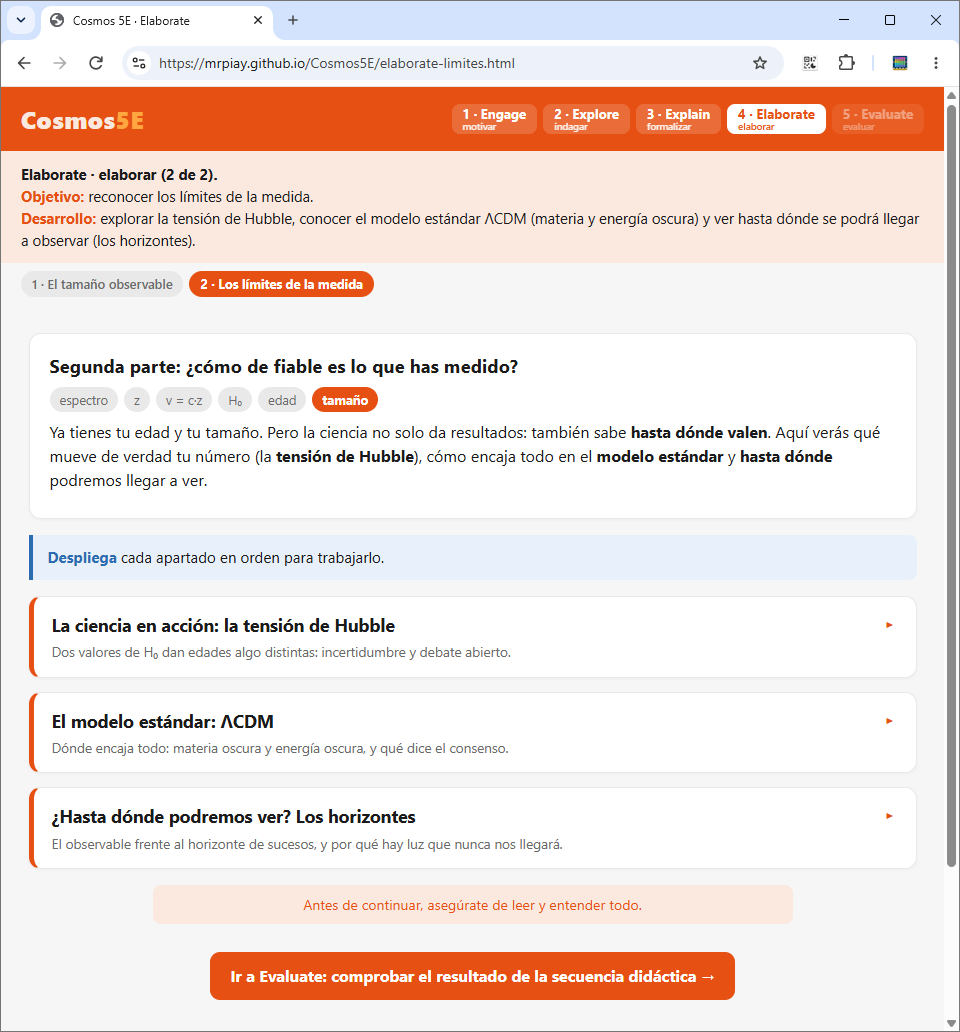
\includegraphics[width=0.82\textwidth]{./Images/web_v2_6_elaborate_limites.png}
\caption{Captura de la sección \textbf{Elaborate}, parte 2: los límites de la medida (tensión de Hubble, $\Lambda$CDM y horizontes).}\label{fig:web-elaborate-limites}
\end{figure}

\subsection{Evaluate (evaluar la comprensión)}

\textbf{Pregunta que la abre:} ¿Cómo hemos medido la edad y el tamaño del universo?

\textbf{Objetivo(s) y OA:} medir el aprendizaje y el \textbf{cambio conceptual} \textit{(OA1--OA7)}.

\textbf{Duración y agrupamiento:} 1 sesión (45 min); individual (cuestionario) y gran grupo (puesta en común).

\subsubsection*{Qué sabemos e ideas previas}

Todo el recorrido conceptual de la secuencia ($z \rightarrow H_{0} \rightarrow$ edad $\rightarrow$ tamaño).

\subsubsection*{Contenido teórico}

No se introduce teoría nueva: se \textbf{sintetiza e integra} el recorrido ---espacio (tamaño) y tiempo (edad) como magnitudes \textbf{inferidas y aproximadas}, no como datos absolutos---, reforzando la naturaleza de la ciencia (medir es inferir con modelos y aproximaciones, y revisar).

\subsubsection*{Desarrollo de la actividad}

El desarrollo paso a paso de esta fase ---cuestionario post y contraste pre$\rightarrow$post, reconstrucción de la cadena de la medida y producto final (explicar el proceso a otra persona)--- se detalla en el diseño de la secuencia (§\ref{sec:evaluate}). Incluye además la \textbf{lectura de las ecuaciones} empleadas ($z=\Delta\lambda/\lambda$, $v=c\,z$, $v=H_{0}\,d$, $t\approx1/H_{0}$, $R\approx c/H_{0}$), aplicando el proceso de lectura del apartado~\ref{sec:ecuaciones} para reconocer el \textbf{origen} y el \textbf{tipo} de cada una. Su implementación en la web se recoge a continuación.

\subsubsection*{Interacción en la web}

\begin{itemize}
\item \textbf{Cuestionario conceptual (post):} el \textbf{mismo instrumento} que el pre de Engage, ahora \textbf{con corrección} y \textbf{contraste pre$\rightarrow$post} (recupera las respuestas guardadas), para que el alumnado perciba su cambio conceptual.
\item \textbf{Repaso del recorrido:} una vista que reconstruye la \textbf{cadena de conceptos} ($z \rightarrow H_{0} \rightarrow$ edad $\rightarrow$ tamaño) para que el alumnado la explique con sus propias palabras.
\item \textbf{Las preguntas del principio:} recupera las cuestiones que Engage dejó \textbf{abiertas} (ahora/pasado, centro, edad y tamaño, la paradoja de Olbers) e invita a responderlas y confirmar la respuesta, cerrando así el ciclo abierto en Engage.
\item \textbf{Lectura interactiva de las ecuaciones:} recorre las cinco ecuaciones accesibles de la secuencia por las seis etapas del proceso de lectura (apartado~\ref{sec:ecuaciones}), en modo revelación y con el foco en su \textbf{origen} y su \textbf{tipo}; al clasificar cada ecuación, hace evaluable la comprensión del proceso, no solo del resultado.
\item \textbf{Cuestionario de verdadero o falso:} afirmaciones que confrontan las ideas erróneas nucleares (§3.5), con retroalimentación inmediata en la web; aporta \textbf{evidencia de aprendizaje} (autoevaluación), complementaria a la puesta en común.
\item \textbf{Plantilla o guion del producto final} (qué explicar y en qué orden).
\end{itemize}

\subsubsection*{Diseño de evaluación}

\textbf{Pre-post} (medición antes y después con los mismos ítems); su aplicación se difiere a la implementación (curso 2026-2027). Referente metodológico: \textcite{gasparini2025}. Los ítems (de opción múltiple, con distractores basados en las ideas erróneas) y la rúbrica de niveles de comprensión se recogen en los instrumentos de evaluación (§4.3), adaptados de inventarios validados de la literatura y de las ideas erróneas (§3.5).

\subsubsection*{Idea errónea que confronta}

Comprobación de que se han superado las seis ideas erróneas nucleares (§3.5): Big Bang como explosión puntual; universo con centro o borde; expansión de los sistemas ligados; corrimiento al rojo como Doppler; confusión materia/energía oscura; energía oscura como «fuerza que empuja». Se comprueba además la superación de la visión de la ciencia como conjunto de hechos cerrados (naturaleza de la ciencia).

\subsubsection*{Espacio--tiempo que se trabaja}

Síntesis integrada de espacio (tamaño) y tiempo (edad): la misma velocidad de la luz que limita lo que vemos fija hasta cuándo podemos mirar atrás.

\subsubsection*{Materiales}

\begin{itemize}
\item \textbf{Cuestionario conceptual} (15 ítems, pre = post) con su clave de corrección (§\ref{sec:instrumentos}).
\item \textbf{Rúbrica A} (trabajo de indagación, Explore) y \textbf{Rúbrica B} (producto final) (§\ref{sec:instrumentos}).
\item \textbf{Plantilla del producto final}.
\end{itemize}

\subsubsection*{Producto de la fase}

Producto final (presentación, póster o vídeo) y autoevaluación del alumnado.

\subsubsection*{Indicadores de logro}

\begin{itemize}
\item \textbf{Mejora pre$\rightarrow$post} en los ítems de ideas erróneas.
\item \textbf{Explica el proceso completo} de medida ($z \rightarrow H_{0} \rightarrow$ edad $\rightarrow$ tamaño), no solo el resultado.
\item Reconoce la edad y el tamaño como magnitudes inferidas y aproximadas (naturaleza de la ciencia).
\item \textbf{Clasifica cada ecuación} de la secuencia por el tipo de conocimiento que expresa (definición, observación o aproximación) y reconoce su origen.
\end{itemize}

\subsubsection*{Proyección de la secuencia}

La secuencia se cierra \textbf{abriendo}: el alumnado constata que quedan preguntas que aún no sabe explicar, y eso ---lejos de ser un fallo--- se presenta como el modo natural en que progresa la ciencia. En lugar de repetir el recorrido, la fase invita a \textbf{dar un paso más} con caminos concretos: perseguir una pregunta abierta (la energía oscura, la forma del universo, la tensión de Hubble o el horizonte de sucesos), profundizar en las ecuaciones de Friedmann ---aprendiendo a \emph{leerlas} aunque su deducción exceda el nivel (apartado~\ref{sec:ecuaciones})---, investigar con datos reales o llevar una de esas preguntas al debate en clase. Así, el final de la secuencia se convierte en un \textbf{principio}, en la línea de §\ref{sec:extension} y del objetivo OA7.

\begin{figure}[htbp]
\centering
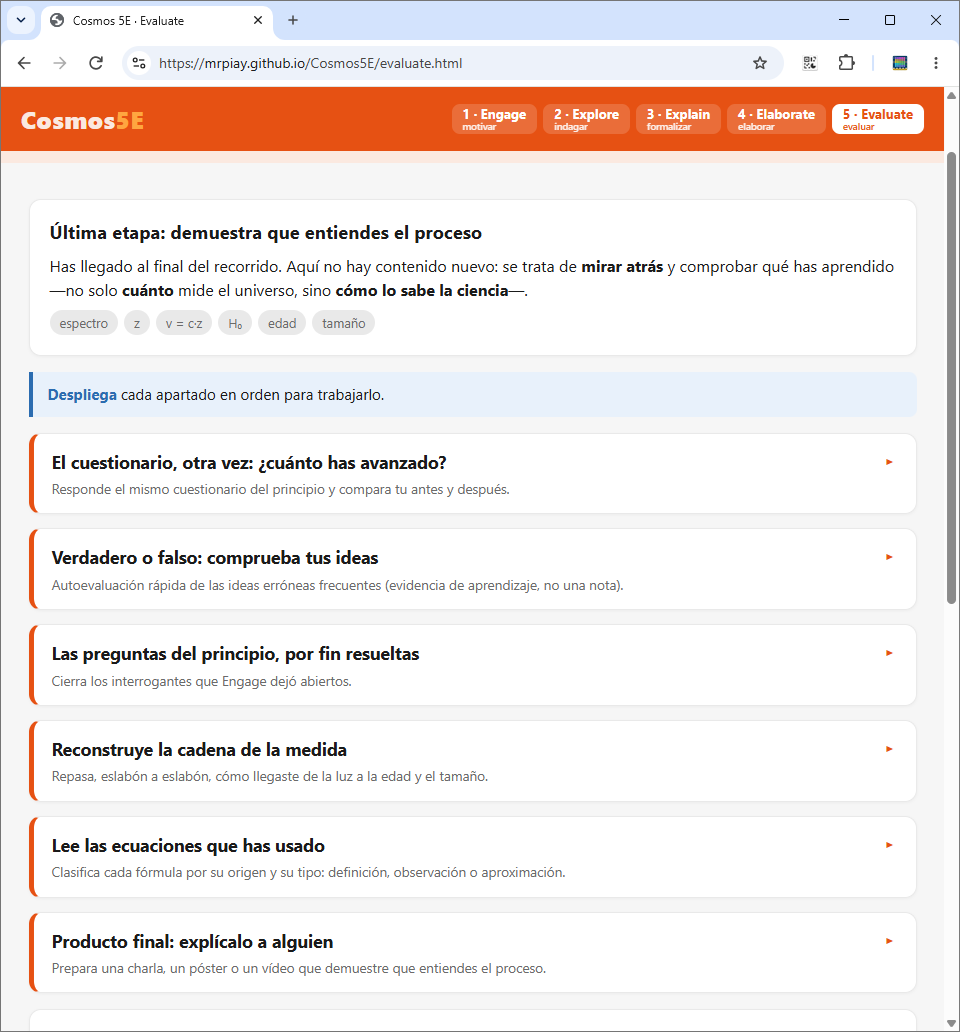
\includegraphics[width=0.82\textwidth]{./Images/web_v2_7_evaluate.png}
\caption{Captura de la sección \textbf{Evaluate} en la web interactiva.}\label{fig:web-evaluate}
\end{figure}

\section{Instrumentos y criterios de evaluación}\label{sec:instrumentos}

La evaluación combina un diseño \textbf{pre-post} de comprensión conceptual con \textbf{dos rúbricas} ---una del proceso de indagación y otra del producto final---, alineados con los objetivos OA1--OA7. El \textbf{cuestionario conceptual} consta de \textbf{15 ítems de opción múltiple} cuyos distractores recogen las seis ideas erróneas nucleares (§3.5) ---Big Bang como explosión puntual, universo con centro o borde, expansión de los sistemas ligados, corrimiento al rojo como Doppler ordinario, confusión entre materia y energía oscura, y energía oscura como «fuerza que empuja»---, junto con otras dificultades documentadas (interpretar $1/H_{0}$ como edad exacta, el radio observable como $c\times$edad, o la visión de la ciencia como conjunto de hechos cerrados). Se administra \textbf{sin cambios} antes (Engage) y después (Evaluate) para estimar la ganancia conceptual, con referente metodológico en \textcite{gasparini2025}. \textbf{Cada ítem se responde siempre} e incluye la opción \emph{«No lo sé / no lo tengo claro»} (para quien no lo tenga claro), de modo que el pre-test queda completo; es el mismo instrumento en ambos momentos. La medida comparable es el \textbf{número de aciertos}. Su versión completa y la clave de corrección se recogen en el anexo de instrumentos. Las \textbf{dos rúbricas} ---\textbf{A}, del trabajo de indagación de Explore, y \textbf{B}, del producto final--- fijan cuatro niveles de logro ---inicial\,(1), en proceso\,(2), adecuado\,(3) y avanzado\,(4)--- en cinco dimensiones cada una, con una \textbf{puntuación total} por suma de las cinco (de 5 a 20); ambas se detallan en el Anexo~\ref{cap:anexo-docente} (Tablas~\ref{tab:rubricaA} y~\ref{tab:rubricaB}).

Junto al cuestionario ---que \emph{mide} la ganancia conceptual pre-post--- y a las rúbricas, la fase Evaluate incorpora un \textbf{cuestionario de verdadero o falso} que confronta las ideas erróneas nucleares: es una \textbf{comprobación conceptual} que aporta \textbf{evidencia de aprendizaje} (autoevaluación con retroalimentación inmediata en la web), al margen del contraste pre-post.

Para facilitar la \textbf{recogida de datos} de la implementación prevista (curso 2026-2027), la web permite \textbf{exportar los resultados} de cada participante ---cuestionario pre y post, el $H_{0}$ medido, las conjeturas de Explore y la explicación de Explain--- en formato \textbf{CSV o JSON}, identificados únicamente con un \textbf{código anónimo} (sin nombres). Así, las respuestas que de otro modo quedarían solo en el almacenamiento local del navegador pueden recuperarse y analizarse con facilidad.

La web incorpora, además, un \textbf{modo de demostración}: rellena automáticamente todas las respuestas y reflexiones y desbloquea las cinco fases, de forma que el docente ---o cualquier persona que revise la herramienta--- puede \textbf{recorrer la secuencia completa sin tener que responder} y \textbf{exportar un conjunto de datos de ejemplo} (en CSV o JSON). Es una utilidad de \textbf{revisión y presentación}, ajena a la actividad del alumnado; su efecto se \textbf{revierte} al reiniciar la secuencia.

\section{Atención a la diversidad y adaptaciones}\label{sec:diversidad}

La secuencia contempla \textbf{andamiajes} y versiones de distinta demanda matemática, de modo que el objetivo central ---comprender el proceso de medida--- sea accesible a todo el alumnado con independencia de su soltura con el cálculo. Como garantía de equidad, cada actividad interactiva dispone de una \textbf{alternativa no digital} equivalente: el diagrama de Hubble puede construirse con datos en papel y una banda elástica que materialice el ajuste de la recta, y la calculadora puede seguirse paso a paso sobre una hoja de trabajo. Las adaptaciones concretas para necesidades específicas quedan \textit{[por concretar]} en función del grupo real.

\section{Plan de implementación (curso 2026-2027)}\label{sec:implementacion}

Se prevé implementar la secuencia en el curso 2026-2027, en un grupo de 2º de Bachillerato, a lo largo de siete sesiones. La recogida de datos pre-post permitirá analizar la ganancia conceptual y el tamaño del efecto, y valorar el cambio en las ideas erróneas. El plan atenderá a las consideraciones éticas oportunas ---información al alumnado, consentimiento y anonimato de los datos---. El grupo concreto, la temporalización definitiva y el detalle del análisis quedan \textit{[por concretar]}.

\subsection{Riesgos y amenazas a la validez}\label{sec:riesgos}

Aunque la validación empírica se difiere, conviene anticipar los principales \textbf{riesgos y amenazas a la validez} del futuro estudio pre-post, con sus mitigaciones:

\begin{itemize}
\item \textbf{Muestra pequeña y sin grupo de control} (un único grupo de aula): limita la validez externa y la inferencia causal. Se asume un carácter \textbf{exploratorio}; los resultados se interpretarán como indicios, no como evidencia concluyente.
\item \textbf{Doble rol docente--investigador} (el autor diseña, imparte y evalúa): posible sesgo del experimentador. Mitigación: uso de \textbf{instrumentos validados} (CosmoCI, \textit{construct map}) y criterios de corrección explícitos.
\item \textbf{Efecto test--retest y deseabilidad social} (mismos ítems antes y después): posible mejora artificial de las puntuaciones. Mitigación: separación temporal suficiente, anonimato de las respuestas y foco en el cambio conceptual, no en la calificación.
\item \textbf{Amenazas internas} (maduración, historia, instrumentación): otros contenidos o eventos del curso podrían influir. Mitigación: acotar la ventana temporal de la secuencia y registrar el contexto de implementación.
\item \textbf{Fidelidad de implementación}: que la secuencia se imparta tal como se diseñó. Mitigación: las fichas de fase y la web interactiva actúan como guion común.
\item \textbf{Dependencia tecnológica}: fallos de equipos o de conectividad. Mitigación: la web es \textbf{offline} (sin conexión) y cada actividad dispone de \textbf{alternativa en papel}.
\end{itemize}

Estas amenazas no invalidan la propuesta ---propia de un trabajo de \textbf{diseño}---, pero orientarán el diseño metodológico de la implementación del curso 2026-2027.

\section{Materiales de la secuencia (anexos)}\label{sec:materiales}

Los materiales de cada fase se han desarrollado como recursos de trabajo que, conforme a la propuesta de §4.1, integran la web interactiva; se incorporan como anexos, con sus enlaces y su atribución o licencia. La Tabla~\ref{tab:materiales} resume los materiales principales por fase.

\begin{table}[ht]
\centering
\caption{Materiales principales por fase.}\label{tab:materiales}
\begin{tabularx}{\textwidth}{|>{\raggedright\arraybackslash}p{2.4cm}|>{\raggedright\arraybackslash}X|}
\hline
\rowcolor{naranja}
{\color{white}\textbf{Fase}} & {\color{white}\textbf{Materiales principales}} \\ \hline
Engage & Reto y pregunta motriz; hitos de la línea de tiempo de la cosmología; simulación interactiva de la paradoja de Olbers; \textbf{cuestionario conceptual} de 15 ítems (con la opción «No lo sé / no lo tengo claro»), pre-test $=$ post-test. \\ \hline
Explore & Espectro(s) de trabajo para medir $z$; conjunto de datos del diagrama de Hubble (galaxias reales con distancia independiente del corrimiento al rojo y velocidad); herramienta de ajuste de recta (y su alternativa con banda elástica); formulario de \textbf{registro de la conjetura}. \\ \hline
Explain & Recogida de la \textbf{explicación del alumnado} (previa a la formalización); calculadora didáctica (cadena $z \rightarrow v \rightarrow H_{0} \rightarrow$ edad, con la conversión de unidades desplegada); gráfico «rebobinar la expansión»; recurso «el corrimiento al rojo de la luz»; calendario cósmico. \\ \hline
Elaborate & \textit{Parte 1 (tamaño):} calculadora (radio de Hubble), simulador del universo observable ($\sim$46\,000 millones de al) y actividad de \textbf{transferencia} a otros valores de $H_{0}$. \textit{Parte 2 (límites):} deslizador de la tensión de Hubble, ficha del modelo $\Lambda$CDM y sección sobre los horizontes. \\ \hline
Evaluate & Cuestionario \textbf{post} (mismos ítems que el pre, con corrección y contraste); \textbf{verdadero/falso} (evidencia de aprendizaje); actividad de lectura de las ecuaciones (apartado~\ref{sec:ecuaciones}); guion del producto final; \textbf{Rúbrica A} (Explore) y \textbf{Rúbrica B} (producto). \\ \hline
\end{tabularx}
\end{table}

\section{El modelo 5E como marco para discusiones abiertas}\label{sec:extension}

La secuencia principal culmina con la edad y el tamaño del universo, pero al determinar el tamaño aflora una pregunta más honda que ninguna fórmula cierra: ¿qué \textbf{forma} tiene el espacio? ¿Es finito o infinito, plano o curvo, y cómo podría saberse estando \textbf{dentro} de él? Esa pregunta ---abierta y sin respuesta de manual--- es el terreno idóneo para un uso distinto del modelo 5E: no como molde de una secuencia completa dirigida a una medida, sino como marco \textbf{breve y provocador} para una \textbf{discusión abierta}, cuyo objetivo no es dominar un contenido, sino despertar la curiosidad y hacer visibles las fronteras del conocimiento.

La lógica del 5E ---implicar, explorar, explicar, elaborar y evaluar--- funciona también \textbf{a menor escala}, en un ciclo corto de una o dos sesiones: se conserva el \textbf{motor} (partir de una provocación, indagar antes de formalizar y cerrar con una síntesis) y se relaja el \textbf{alcance} y, sobre todo, la \textbf{evaluación}, que se vuelve \textbf{formativa y reflexiva} ---el logro no es «acertar», sino formular buenas preguntas y reconocer los límites de lo que se sabe---. Un ejemplo natural de este uso, \textbf{opcional} y a modo de enriquecimiento ---fuera de la secuencia principal, por lo que no se incorpora a la web para no sobrecargarla---, sería un ciclo breve sobre la \textbf{geometría del universo}: partiendo del tamaño ya calculado, preguntar si el espacio es finito o infinito, plano o curvo; introducir la \textbf{densidad crítica} (con la lógica de la velocidad de escape) y distinguir el \textbf{destino} del universo (expansión eterna, límite o recolapso) de su \textbf{geometría} ---un resultado de la Relatividad General que se \emph{enuncia}, no se deduce, y cuyas ecuaciones pueden \emph{leerse} con la metodología del §\ref{sec:ecuaciones} y el Anexo~\ref{cap:anexo-ecuaciones}---. Aunque las medidas indican una curvatura \textbf{plana}, la discusión deja abiertas las grandes preguntas de fondo ---el tamaño total (¿finito o infinito?) y los modelos de expansión y destino---. Este formato resulta especialmente útil como \textbf{cierre} de la unidad o como estímulo de \textbf{vocaciones científicas} (OA7): la ciencia no termina en el resultado, sino que se abre en él, y el final de la secuencia principal se convierte en un principio.

\section{Las ecuaciones de la cosmología: metodología didáctica}\label{sec:ecuaciones}

Este apartado presenta una metodología didáctica para leer e interpretar ecuaciones y la aplica a las principales expresiones matemáticas utilizadas para estimar la edad y el tamaño del universo. Su objeto no es que el alumnado \emph{derive} dichas ecuaciones ---una tarea que excede el nivel de Bachillerato---, sino que aprenda a \emph{interpretarlas}: a comprender qué afirman, de qué dependen y qué tipo de conocimiento expresan.

Comprender la cosmología exige interpretar sus ecuaciones, que son el lenguaje en el que se expresa con exactitud el conocimiento científico: una relación como $v = H_{0}\,d$ es lo que convierte una observación ---el alejamiento de las galaxias--- en una estimación de la edad del universo. Sin embargo, para gran parte del alumnado de 2º de Bachillerato la ecuación constituye un obstáculo: los símbolos se manipulan mecánicamente ---se despejan, se sustituyen, se calculan--- sin llegar a interpretarse, y la fórmula acaba funcionando como una caja negra que produce resultados sin comprensión.

Esa dificultad suele afrontarse derivando las ecuaciones, es decir, reconstruyendo el razonamiento que conduce hasta ellas; pero en cosmología esa vía es inviable. Las expresiones fundamentales ---como las ecuaciones de Friedmann, la densidad crítica o la aceleración de la expansión--- proceden de la relatividad general. Sin embargo, no pueden omitirse, porque sostienen las magnitudes que la secuencia pretende estimar. Ante ecuaciones imprescindibles cuya derivación queda fuera del alcance del alumnado ---una circunstancia que hace de la cosmología un terreno idóneo para este enfoque---, el objetivo de aprendizaje se replantea: no derivarlas, sino aprender a leerlas e interpretarlas.

Con este fin se propone un \textbf{proceso de lectura} de seis etapas ---detallado más adelante--- que convierte el lenguaje simbólico en significado conceptual y culmina en la pregunta por el \emph{tipo} de conocimiento que la ecuación representa. El enfoque se apoya en la conversión entre registros semióticos \parencite{duval2006}, en la alfabetización matemática de PISA \parencite{oecd2019} y en la naturaleza de la ciencia \parencite{lederman1992}, y se integra en la secuencia 5E: cada ecuación que el alumnado emplea en las fases \emph{Explore}, \emph{Explain} y \emph{Elaborate} se analiza con el mismo procedimiento, fijo y repetible. El método se aplica, además, a las ecuaciones de fondo procedentes de la relatividad general ---las de Friedmann--- que sostienen el modelo pero que \textbf{no se calculan ni se derivan en el aula}: se \emph{leen} como ejemplo culminante del enfoque ---son, de hecho, sus únicos casos de tipo \emph{Derivación}---, no como contenido nuevo que el alumnado deba dominar. Así, comprender las fórmulas deja de ser un requisito implícito y se convierte en una tarea observable ---que puede plantearse, guiarse y calificarse---: un objetivo de aprendizaje explícito y evaluable, en el que las seis etapas funcionan como una rúbrica de comprensión.

\subsection{Las etapas del proceso de lectura}

El proceso de lectura se recorre en seis etapas, planteadas como preguntas que se formulan siempre en el mismo orden ante cualquier ecuación. Ese orden no es casual: conduce progresivamente desde la interpretación del lenguaje matemático hasta la valoración del tipo de conocimiento que expresa:

\begin{enumerate}
  \item \textbf{Símbolos.} ¿Qué representa cada símbolo y en qué unidades se expresa?
  \item \textbf{Relación.} ¿Cómo se vinculan las magnitudes entre sí? ¿La dependencia es directa, inversa\ldots?
  \item \textbf{Sentido.} ¿Qué indican los signos ---crecimiento, atracción, cancelación--- y qué significan? En las ecuaciones con varios términos, ¿cómo se leen en conjunto?
  \item \textbf{Propósito.} ¿Qué mide o predice la ecuación? ¿Para qué sirve?
  \item \textbf{Origen.} ¿De qué teoría o de qué observación procede? Se identifica su procedencia, sin reconstruir su derivación.
  \item \textbf{Tipo.} ¿Qué clase de afirmación es la ecuación?
\end{enumerate}

La sexta pregunta se responde clasificando la ecuación en una de cuatro categorías, que precisan la naturaleza del conocimiento que expresa y el grado de confianza que puede atribuírsele:

\begin{itemize}
  \item \textbf{Definición.} La ecuación se limita a nombrar o convenir una magnitud; no se demuestra, se establece.
  \item \textbf{Observación.} Expresa un patrón medido en la naturaleza, no deducido de una teoría; su validez descansa en los datos.
  \item \textbf{Aproximación.} Es válida únicamente bajo ciertas condiciones, que deben explicitarse; fuera de ellas deja de aplicarse.
  \item \textbf{Derivación.} Se obtiene de una teoría más general; no se reconstruye aquí su derivación, pero se identifica su origen.
\end{itemize}

Las cinco primeras preguntas permiten interpretar el contenido matemático de la ecuación; la sexta desplaza la atención desde lo que la ecuación dice hacia la razón por la que puede aceptarse como conocimiento científico.

\subsection{Un ejemplo: la ley de Hubble}

A modo de ilustración, el proceso se aplica a la ley de Hubble-Lemaître, $v = H_{0}\,d$, ecuación central de la secuencia:

\begin{itemize}
  \item \textbf{Símbolos.} $v$ es la velocidad de recesión de una galaxia (km/s); $d$, su distancia (Mpc); $H_{0}$, la constante de Hubble (km/s por Mpc).
  \item \textbf{Relación.} Directa: cuanto mayor es la distancia, mayor es la velocidad de alejamiento.
  \item \textbf{Sentido.} La velocidad de recesión es positiva y crece con la distancia para las galaxias suficientemente lejanas; en $d = 0$ resulta $v = 0$: no hay recesión respecto del propio observador.
  \item \textbf{Propósito.} Representada gráficamente para muchas galaxias, la pendiente de la recta proporciona el valor de $H_{0}$, a partir del cual se estima después la edad del universo.
  \item \textbf{Origen.} Es una \textbf{relación empírica}: el patrón que Hubble observó en 1929 al relacionar la velocidad y la distancia de las galaxias; es, además, consistente con los modelos cosmológicos homogéneos de expansión.
  \item \textbf{Tipo.} \emph{Observación.} Es un hecho empírico; interpretar que implica la expansión del universo constituye una lectura del modelo cosmológico, no una consecuencia lógica de la fórmula.
\end{itemize}

Esta lectura transforma una ecuación que el alumnado tendería simplemente a «usar» ---despejar $H_{0}$, sustituir valores--- en una afirmación que comprende: sabe qué relaciona, para qué sirve, de dónde procede y qué alcance tiene. El anexo~\ref{cap:anexo-ecuaciones} recoge esta lectura para las nueve ecuaciones de la cosmología: las cinco que vertebran la medida en la secuencia y las cuatro de fondo ---las de Friedmann--- que allí solo se leen, sin derivarlas.

\chapter{Conclusiones y líneas futuras}\label{cap:conclusiones}

Este capítulo cierra el trabajo revisando en qué medida se han alcanzado los objetivos planteados en el Capítulo~\ref{cap:intro}, señalando las aportaciones que lo distinguen, reconociendo sus limitaciones y proyectando su continuidad. Conviene recordar el marco desde el que se leen estas conclusiones: se trata de un \textbf{Trabajo de Fin de Máster de diseño}, cuyo producto es una secuencia didáctica fundamentada y sus materiales, no un estudio empírico de aula. Por ello, los resultados que aquí se recogen se refieren al proceso de diseño, a la coherencia interna de la propuesta y a su alineación con la literatura y con el currículo; su eficacia sobre el aprendizaje es una hipótesis razonada que deberá contrastarse en la implementación prevista.

\section{Grado de consecución de los objetivos}

El \textbf{objetivo general} ---diseñar una secuencia didáctica basada en el modelo 5E para la determinación de la edad y el tamaño del universo, empleando la expansión y la ley de Hubble-Lemaître como vía de medida--- se ha cumplido: el trabajo entrega una secuencia completa para 2.º de Bachillerato que culmina, precisamente, en la estimación de esos dos valores a partir de observaciones reales. Los objetivos específicos se han abordado del modo siguiente:

\begin{itemize}
\item \textbf{OE1 y OE2} (Cap.~\ref{cap:revision}). La revisión sistematizada de la literatura sobre enseñanza de la cosmología moderna en secundaria se ha materializado en el análisis de 78 fuentes, organizadas en diez categorías de estrategia y contexto, con identificación de los contenidos más tratados, las estrategias empleadas y las dificultades conceptuales documentadas. De esa síntesis se extrajeron los elementos transferibles y se asignaron a las cinco fases del modelo 5E.

\item \textbf{OE3} (Cap.~\ref{cap:revision}). El cotejo de esos contenidos con el currículo de Física que imparte el autor situó la propuesta en Pearson Edexcel IAL (Topic~11, «Astrophysics and Cosmology»), que encaja casi punto por punto con el tema y fija el nivel en 2.º de Bachillerato; la PCE UNED se valoró y quedó descartada como marco de la propuesta.

\item \textbf{OE4} (Cap.~\ref{cap:propuesta}). Sobre esa base se diseñó la secuencia 5E, seleccionando qué contenidos incluir, qué estrategias resultaban más adecuadas para cada fase y qué ideas erróneas debían abordarse de forma explícita, con una estructura articulada en torno a una pregunta motriz y a una progresión de conceptos que conduce del corrimiento al rojo hasta la edad y el tamaño del universo.

\item \textbf{OE5} (Cap.~\ref{cap:desarrollo}). Se diseñaron los instrumentos de evaluación: dos rúbricas de cuatro niveles, un cuestionario conceptual pre-post adaptado de inventarios validados \parencite{gasparini2025} y un instrumento formativo integrado en la web interactiva (confrontación de ideas erróneas mediante verdadero/falso), previendo su aplicación en la implementación del curso 2026-2027.

\item \textbf{OE6} (Cap.~\ref{cap:desarrollo}). Se propuso una metodología didáctica para la lectura e interpretación de las ecuaciones que sustentan la medida ---no para su deducción formal---, articulada en seis etapas y aplicada al catálogo de ecuaciones de la secuencia, como aportación transversal recogida en el apartado correspondiente y en el anexo de ecuaciones.
\end{itemize}

En conjunto, los seis objetivos específicos se consideran alcanzados en el plano del diseño, que es el alcance declarado del trabajo.

\section{Aportaciones del trabajo}

Más allá de entregar una secuencia 5E coherente y fundamentada, el trabajo aporta dos elementos que lo singularizan.

El primero es la \textbf{web interactiva de acompañamiento \textit{Cosmos 5E}}: una herramienta offline, de código abierto y sin dependencias, que recorre las cinco fases y ofrece como piezas centrales una calculadora didáctica y un diagrama de Hubble construido sobre datos reales \parencite{steer2017}. Su principio de diseño es no funcionar como una caja negra: cada paso explica qué se va a hacer, por qué interviene y qué significa el resultado, mostrando la cadena de la medida con sus unidades desplegadas. El uso de distancias y velocidades reales, en lugar de valores fabricados, ancla la propuesta en la práctica científica auténtica y permite que el alumnado obtenga su propia estimación de la constante de Hubble y, a partir de ella, de la edad y el tamaño del universo.

El segundo es la \textbf{metodología para la lectura e interpretación de ecuaciones}, organizada en seis etapas (símbolos, relación, sentido, propósito, origen y tipo). Concebida como articulación operativa de principios ya establecidos ---la conversión entre registros de representación \parencite{duval2006}, la alfabetización matemática y la naturaleza de la ciencia---, ofrece un procedimiento fijo y repetible que convierte la comprensión de una fórmula en una tarea observable, que puede plantearse, guiarse y calificarse. Aunque aquí se aplica a la cosmología ---un banco de pruebas idóneo, por cuanto sus ecuaciones son imprescindibles pero indeducibles a este nivel---, la metodología es transferible a otros contenidos de la física.

\section{Limitaciones}

El trabajo presenta limitaciones que conviene explicitar y que, en su mayoría, derivan de su naturaleza de propuesta de diseño.

\begin{itemize}
\item \textbf{Ausencia de pilotaje.} Al no implementarse dentro del propio TFM, la eficacia de la secuencia sobre el aprendizaje no se ha comprobado empíricamente: es una hipótesis fundamentada, no un resultado.

\item \textbf{Contexto único.} El diseño se ancló en un currículo concreto (Edexcel IAL), lo que favorece su encaje pero limita la generalización directa a otros marcos, como la PCE UNED, que quedó fuera de la propuesta.

\item \textbf{Validación pendiente de la web y de los instrumentos.} La herramienta no se ha sometido a una evaluación de usabilidad y accesibilidad con alumnado real, y los instrumentos de evaluación, aunque adaptados de inventarios validados, no se han validado psicométricamente en el contexto de aplicación.

\item \textbf{Carácter didáctico del conjunto de datos.} El conjunto de galaxias del diagrama de Hubble es una selección con fines didácticos, no un muestreo científico; se ha priorizado la claridad del ajuste lineal y la aparición de las velocidades peculiares como lección, sobre la exhaustividad.

\item \textbf{Régimen simplificado.} La propuesta se mantiene deliberadamente en el régimen lineal de la ley de Hubble y en la aproximación de la edad como inversa de la constante de Hubble; los tratamientos exactos quedan señalados como matiz o como ampliación, no desarrollados.
\end{itemize}

\section{Líneas futuras}

La continuación natural del trabajo es su \textbf{implementación en el aula durante el curso 2026-2027}, en la ventana ya identificada del currículo de Física del autor, con la aplicación de los instrumentos diseñados en un esquema de evaluación \textbf{pre-post}. Esa experiencia permitiría contrastar la hipótesis central del trabajo y recoger evidencia sobre la comprensión efectiva de la edad y el tamaño del universo.

De ella se derivan otras líneas:

\begin{itemize}
\item \textbf{Validación y mejora de la web}, incorporando la observación del uso real del alumnado, criterios de accesibilidad y, en su caso, nuevas actividades o datos.

\item \textbf{Transferencia a otros contextos}, adaptando la secuencia a marcos curriculares distintos y extendiendo la metodología de lectura de ecuaciones a otros bloques de la física.

\item \textbf{Ampliación de nivel}, para itinerarios más avanzados, abordando las ecuaciones de Friedmann y la geometría del universo con mayor profundidad de la que admite el nivel de referencia.

\item \textbf{Integrar más actividades y elementos de evaluación en la web}: llevar a la herramienta actividades que hoy se apoyan en materiales complementarios y los elementos de evaluación ---registro de las respuestas, aplicación de las rúbricas y seguimiento del progreso del alumnado---, de modo que la secuencia completa y su evaluación puedan realizarse y quedar registradas en línea.

\item \textbf{Entorno docente en la web}: incorporar a la propia herramienta una sección docente ---con navegación libre por las fases, la guía de sesiones, los instrumentos y sus claves de corrección, y los datos descargables--- e integrar en la misma aplicación los dos modos de uso, el del alumnado y el del profesorado. De este modo, los materiales de reproducibilidad que este trabajo recoge en los anexos quedarían también accesibles en línea, sin necesidad de preparar nada por separado.
\end{itemize}

\section{Reflexión final}

La secuencia diseñada busca que el alumnado no reciba la edad y el tamaño del universo como cifras cerradas, sino que las reconstruya siguiendo el mismo camino que la ciencia: observar, medir, interpretar y, sobre todo, comprender qué significan los números y de dónde proceden. En coherencia con el espíritu del modelo 5E, el final de la secuencia se plantea como un principio: al término del recorrido, el estudiante debería quedarse no solo con respuestas, sino con mejores preguntas. Si la propuesta consigue que alguien mire el cielo y entienda que su oscuridad, su antigüedad y su extensión son cosas que se pueden medir y razonar, habrá cumplido su verdadero propósito.

%-------------------- ANEXOS --------------------%
\appendix
\chapter{Fuentes de la revisión exploratoria (Elicit Pro)}\label{cap:anexo1}

Se recoge el conjunto de \textbf{fuentes} identificadas en la búsqueda exploratoria (Elicit Pro), conservando su \textbf{numeración original}. Los índices que aparecen entre corchetes en la tabla de análisis del Capítulo~2 (Tabla~\ref{tab:analisis}) remiten al número correspondiente de este listado.

{\footnotesize
\begin{enumerate}\setlength{\itemsep}{2pt}
\item Xu B, Su J, Wang W (2018) An expanding balloon: a small universe. The Physical Educator. \url{https://doi.org/10.1088/1361-6552/aad71f}
\item Suárez Á (2025) Exploring cosmology: a simple experiment to illustrate the cosmological principle and the Hubble–Lemaître Law. The Physical Educator. \url{https://doi.org/10.1088/1361-6552/adac24}
\item Marshall O, Tojeiro R, Weijmans A (2022) Demonstrating cosmological and Doppler redshift in the classroom. 4th Symposium on Space Educational Activities. \url{https://doi.org/10.5821/conference-9788419184405.098}
\item Possel M (2020) Interpretations of cosmic expansion: anchoring conceptions and misconceptions. The Physical Educator. \url{https://doi.org/10.1088/1361-6552/aba3b1}
\item Hyde J (2021) Exploring Hubble Constant Data in an Introductory Course. The Physics Teacher. \url{https://doi.org/10.1119/10.0003654}
\item Raymundo IBP, Ferreira LO de OB, Mello1 MMW, Pigozzo C (2022) Estimando a aceleração da expansão do Universo com o SimECosmo. Revista Brasileira de Ensino de Física. \url{https://doi.org/10.1590/1806-9126-rbef-2022-0143}
\item Lochner J (2009) Extra! Extra! Read All about the Universe! The Science Teacher
\item Pereira JAM (2019) Introducing dark energy in the classroom using paradoxes. Journal of Physics: Conference Series. \url{https://doi.org/10.1088/1742-6596/1286/1/012008}
\item Nunes G, Damasio F (2025) Contribuições para o desenvolvimento da cosmologia moderna: A Física na Escola. \url{https://doi.org/10.59727/fne.v22i1.212}
\item Salimpour S, Tytler R, Fitzgerald M, Eriksson U (2023) Is the Universe Infinite? Characterising a Hierarchy of Reasoning in Student Conceptions of Cosmology Concepts Using Open-Ended Surveys. Journal for STEM Education Research. \url{https://doi.org/10.1007/s41979-023-00088-8}
\item Woithe J, Kersting M (2020) Bend it like dark matter! The Physical Educator. \url{https://doi.org/10.1088/1361-6552/abe09c}
\item Aretz S, Borowski A, Schmeling S (2017) Development and Evaluation of a Construct Map for the Understanding of the Expansion of the Universe. \url{https://doi.org/10.18452/8216}
\item Gasparini A, Mueller A, Stern F, Weiss L (2025) Cosmology and general relativity in upper secondary school through new targeted teaching materials: A study on student learning and motivation. Physical Review Physics Education Research. \url{https://doi.org/10.1103/ss9c-lkpj}
\item Dua YS, Blair D, Kaur T, Choudhary R (2020) Can Einstein’s Theory of General Relativity be Taught to Indonesian High School Students? Jurnal Pendidikan IPA Indonesia. \url{https://doi.org/10.15294/jpii.v9i1.22468}
\item Aguiar R (2010) Tópícos de Astrofísica e Cosmologia: uma aplicação de Física Moderna e Contemporânea no Ensino Médio. \url{https://doi.org/10.11606/D.81.2010.TDE-25012011-112911}
\item Souza DCP de, Teixeira R (2022) MATÉRIA ESCURA E ENERGIA ESCURA EM ATIVIDADES DE DIVULGAÇÃO CIENTÍFICA. Revista Eletrônica Debates em Educação Científica e Tecnológica. \url{https://doi.org/10.36524/dect.v11i01.1513}
\item Lin B.-H. (2011). [Tesis en chino: el nuevo currículo de Física de 1.º de bachillerato ---fenómenos cuánticos y cosmología---; valoración del profesorado y preparación docente]. National Taiwan University. \url{https://doi.org/10.6342/NTU.2011.01400}
\item Skolimoski KN (2014) Cosmologia na teoria e na prática: possibilidades e limitações no ensino. \url{https://doi.org/10.11606/D.81.2014.TDE-09042015-154106}
\item Jardim WT, Guerra A (2013) Minicurso de cosmologia na formação de professores; dificuldades na ampliação de propostas para o ensino médio
\item McGoran D (2021) Developing a Cosmology Unit for Year 10 Students to Determine Hubble’s Constant Using Gravitational Waves. Physical Sciences Forum. \url{https://doi.org/10.3390/ecu2021-09316}
\item Salimpour S, Tytler R, Doig B, et al (2022) Conceptualising the Cosmos: Development and Validation of the Cosmology Concept Inventory for High School. International Journal of Science and Mathematics Education. \url{https://doi.org/10.1007/s10763-022-10252-y}
\item Dole H (2024) Cosmology Ruler Bookmark for Teaching and Outreach Purposes (Pen-and-pencil cosmological ruler calculator for everyone, especially students)
\item Hollow R (2005) Syllabus Requirements for VCE Astronomy and Astrophysics
\item Tortoriello F, Benedetto E, D'acunto I (2025) Mathematics and physics at work: the study of cosmological functions in a high school. The Physical Educator. \url{https://doi.org/10.1142/s2661339525500131}
\item Pereira J (2019) Introducing dark energy in the classroom using paradoxes. Journal of Physics: Conference Series. \url{https://doi.org/10.1088/1742-6596/1286/1/012008}
\item Huwe P, Field SE (2015) Modern Gravitational Lens Cosmology for Introductory Physics and Astronomy Students. The Physics Teacher. \url{https://doi.org/10.1119/1.4917429}
\item Pössel M (2018) Teaching cosmology with special relativity: piecewise inertial frames as a model for cosmic expansion. European journal of physics. \url{https://doi.org/10.1088/1361-6404/aaf2f7}
\item Colantonio A, Marzoli I, Testa I, Puddu E (2019) An investigation on conceptual understanding about cosmology. Proceedings of the International Astronomical Union. \url{https://doi.org/10.1017/S174392132100096X}
\item Brems S, Schafer BM, Bucciantini N, et al (2018) The Dark Universe - Exercises and Proceedings from the German-Italian WE Heraeus Summer School held in 2017 in Heidelberg. arXiv: Cosmology and Nongalactic Astrophysics
\item Etkina E, Lawrence M, Charney J (1999) Introducing astrophysics research to high school students. Physics Education. \url{https://doi.org/10.1088/0031-9120/34/5/305}
\item Bartlett S (2018) Hubble Plots in High School. Robotic Telescopes, Student Research and Education Proceedings, Vol 1, No 1. \url{https://doi.org/10.32374/RTSRE.2017.024}
\item Murdin P (1991) The Great Attractor: at the limits of Hubble's Law of the expanding Universe. Physics Education. \url{https://doi.org/10.1088/0031-9120/26/6/007}
\item Trotta R, Hajas D, Camargo-Molina JE, et al (2020) Communicating cosmology with multisensory metaphorical experiences. \url{https://doi.org/10.22323/2.19020801}
\item Çoban G, Sengoren SK (2011) A Simple Way of Modeling the Expansion of the Universe: What Does Light Tell Us?. Science Activities: Classroom Projects and Curriculum Ideas. \url{https://doi.org/10.1080/00368121.2010.502549}
\item Etkina E, Lawrence M, Charney J (1999) Introducing astrophysics research to high school students. Physics Education. \url{https://doi.org/10.1088/0031-9120/34/5/305}
\item Stoppel H (2021) Making particle physics and cosmology accessible for high school students. International Conference on Rebooting Computing. \url{https://doi.org/10.22323/1.395.1369}
\item Linton J (2012) Cosmological expansion. Physics Education. \url{https://doi.org/10.1088/0031-9120/47/1/96}
\item Pereira R de S, Tavares MDS, Moreira E, Moucherek FM de O (2020) Astronomia e Cosmologia: as suas implicações e mistérios para a Física Fundamental
\item Jones MH, Lambourne R, Serjeant S (2015) An Introduction to Galaxies and Cosmology (2nd ed)
\item Pössel M (2018) Relatively complicated? Using models to teach general relativity at different levels. arXiv: General Relativity and Quantum Cosmology
\item Coban GU, Sengoren SK (2011) A Simple Way of Modeling the Expansion of the Universe: What Does Light Tell Us? Science Activities. \url{https://doi.org/10.1080/00368121.2010.502549}
\item Ford J, Stang J, Anderson CL (2015) Simulating Gravity: Dark Matter and Gravitational Lensing in the Classroom. The Physics Teacher. \url{https://doi.org/10.1119/1.4935771}
\item Caldas RL, Siqueira AB de O (2019) Potentially meaningful teaching unit on Cosmology in the vision of the teacher of fundamental and average education. Journal of Physics: Conference Series. \url{https://doi.org/10.1088/1742-6596/1286/1/012064}
\item Bondell J (2025) Bridging Scientists and Students with Regional School Partnerships. Proceedings of The XVIth Quark Confinement and the Hadron Spectrum Conference — PoS(QCHSC24). \url{https://doi.org/10.22323/1.483.0025}
\item Ritz E, Chow N (2018) Teaching The Expanding Universe. The School science review
\item Postiglione A, Curceanu C, Bertelli S (2026) From students to experts: an example of flipped classroom during the INFN-INSPYRE International School. Proceedings of The European Physical Society Conference on High Energy Physics — PoS(EPS-HEP2025). \url{https://doi.org/10.22323/1.485.0610}
\item Arcadias L, Corbet R, Booth E (2025) Astro-Animation - How Artists and Scientists Envision the Universe. Mutual Images Journal. \url{https://doi.org/10.32926/2025.ACB}
\item Ferreira M, Couto RVL do, Filho OL da S, et al (2021) Ensino de astronomia: uma abordagem didática a partir da Teoria da Relatividade Geral. Revista Brasileira de Ensino de Física. \url{https://doi.org/10.1590/1806-9126-rbef-2021-0157}
\item Smecker-Hane T, Naray RKD (2010) The UCI COSMOS Astronomy \& Astrophysics Program for Talented High School Students
\item Wiesner M, Sederberg D, Lang R (2020) Simulating a Dark Matter Detector in a Physics Classroom. The Physics Teacher. \url{https://doi.org/10.1119/1.5144792}
\item Veen JVD, Lubin P, Natoli P, Seiffert M (1998) Small-scale anisotropies: The final frontier. The Physics Teacher. \url{https://doi.org/10.1119/1.880137}
\item Girola R, Santos M (2011) A DIDACTIC PROPOSAL IN THE LEARNING OF ASTRONOMY THROUGH PARADIGMATIC CHANGES. Revista Mexicana De Astronomia Y Astrofisica
\item Simionato S (2020) Didaktik der Physik-Beiträge zur DPG-Frühjahrstagung-Jahresband 2020
\item Faye S, Faye M (2009) Teaching astronomy and astrophysics with Hands-On-Universe and SalsaJ: stars, planets, exoplanets and dark matter. Proceedings of the International Astronomical Union. \url{https://doi.org/10.1017/S1743921311003073}
\item Huggins E (2013) Vacuum Energy and Inflation: 1. A Liter of Vacuum Energy. The Physics Teacher. \url{https://doi.org/10.1119/1.4818374}
\item Andrade GL, Santos RA dos, Santana IL, Takiya C (2020) SOBRE A RELAÇÃO ENTRE A FÍSICA DE PARTÍCULAS E A COSMOLOGIA: UMA ABORDAGEM E PROPOSTA DIDÁTICA PARA O ENSINO MÉDIO. \url{https://doi.org/10.51162/brc.dev2020-00041}
\item Casamiquela L, Cita VM de la, Ràfols IP, Fàbrega SR (2022) Finestres al cel. 4th Symposium on Space Educational Activities. \url{https://doi.org/10.5821/conference-9788419184405.089}
\item McKinnon DH, Nolan CJP (2000) Cosmology on the Internet: Distance Education for the Gifted and Talented. Publications Astronomical Society of Australia. \url{https://doi.org/10.1071/AS00133}
\item Araújo ACS, Júnior JAD, Romeu MC (2023) Abordagem metodológica Team-based Learning: estratégia facilitadora para o ensino de Cosmologia. Revista de Ensino de Ciências e Matemática. \url{https://doi.org/10.26843/rencima.v14n4a12}
\item Tuveri M, Fadda D, Fanti V, Bonivento W (2022) When physics meets philosophy again: the “Gravitas” project. Proceedings of 41st International Conference on High Energy physics — PoS(ICHEP2022). \url{https://doi.org/10.22323/1.414.0392}
\item Pimbblet K, Newman J (2003) Ex-nihilo II: examination syllabi and the sequencing of cosmology education. Physics Education. \url{https://doi.org/10.1088/0031-9120/38/3/307}
\item Horvath J, Moraes P (2021) Should we teach general relativity in high school? Why and how? Astronomy Education Journal. \url{https://doi.org/10.32374/aej.2021.1.1.008}
\item Carmesin H (2018) A Model for the Dynamics of Space - Expedition to the Early Universe -
\item Griffiths M (2009) The immortal ant and the expanding balloon. Teaching Mathematics and Its Applications. \url{https://doi.org/10.1093/TEAMAT/HRP009}
\item Pössel M (2021) Models and analogies in teaching general relativity. Teaching Einsteinian Physics in Schools. \url{https://doi.org/10.4324/9781003161721-13}
\item Bottino B (2021) The Outreach and Education program of the Darkside experiment. Journal of Physics: Conference Series. \url{https://doi.org/10.1088/1742-6596/2156/1/012164}
\item Diatlov Yu., Priadko N., Liubchykova D. (2025). [En ucraniano: aplicación práctica de los materiales de una escuela de astrofísica para la enseñanza de la física y la astronomía en la Nueva Escuela Ucraniana]. Physics and Educational Technology. \url{https://doi.org/10.32782/pet-2025-2-4}
\item Tuveri M, Fadda D, Fanti V, Bonivento W (2022) When gravity meets philosophy again: the Gravitas project
\item Navone HD, Scancich M, Vazquez R (2011) ASTROFÍSICA ESCOLAR: BRINCANDO COM DADOS OBSERVACIONAIS. \url{https://doi.org/10.37156/RELEA/2011.11.081}
\item Paganotti A, Gomes G, Vieira GC, Silva R de CVL da (2022) Características das principais dificuldades encontradas nas escolas públicas de Minas Gerais para o ensino de astronomia e cosmologia aos alunos do ensino médio. Brazilian Journal of Development. \url{https://doi.org/10.34117/bjdv8n8-270}
\item Pimbblet KA, Newman JC (2003) Ex-nihilo II: examination syllabi and the sequencing of cosmology education. Physics Education. \url{https://doi.org/10.1088/0031-9120/38/3/307}
\item Santos RF (2014) Noções de astrofísica e de cosmologia moderna nas aulas de física do ensino médio: uma sequência didática a partir do Paradoxo de Olbers
\item Navone H, Scancich M, Vazquez R (2011) Astrophysics In Schools: Playing With Observational Data
\item Oliveira SK de (2019) Espectroscopia para o ensino de física moderna e cosmologia
\item Hollow R (2006) Concepts for The Cosmic Engine
\item Gramstad E, Ould-Saada F, Bugge MK (2018) The challenge of explaining new physics concepts and phenomena. \url{https://doi.org/10.22323/1.314.0556}
\item Lubowich D, Shupla C (2014) Edible Earth and Space Science Activities
\item Azeredo EC (2018) Proposta didática de ensino de cosmologia com o auxílio de jogos e teatro
\item Noronha A, Bagdonas A, Gurgel I (2018) Is the Electron Real? Who Discovered the Expanding Universe? Debating Nonconsensus Topics of Nature of Science in Science Classrooms. \url{https://doi.org/10.1007/978-3-319-74036-2_7}
\item Rodríguez B (2011) Representaciones mentales de docentes sobre el universo : los modelos cosmológicos que lo explican y aplicación de una estrategia metodológica para promover su evolución. \url{https://doi.org/10.36443/10259/84}
\item Carmesin H, Carmesin E (2014) How Old is the Universe
\item Novotný J, Svobodová J (2017) What are science teacher’s ideas about the universe? \url{https://doi.org/10.1063/1.4974401}
\item Cardona-Rodriguez G, Roncancio JDR, Giraldo M (2016) Construcción de un diagrama de Hubble: Una herramienta para la Enseñanza de la Astronomía - Building a Hubble Diagram: A Tool for Teaching Astronomy. \url{https://doi.org/10.14483/UDISTRITAL.JOUR.RC.2016.24.A2}
\item Carmesin H (2019) Didaktik der Physik-Beiträge zur DPG-Frühjahrstagung-Jahresband 2019
\item Rodríguez G, Reyes J, Giraldo M (2016) Construcción de un diagrama de Hubble: una herramienta para la enseñanza de la astronomía Construction of a Hubble Diagram: A Tool for Teaching Astronomy Construção de um Diagrama de Hubble: Uma Ferramenta para Ensino de Astronomía
\item Bartlett S (2018) Hubble Plots in High School: The Faulkes Telescope Project
\item Hemenway M, Jogee S, Fricke K, et al (2008) Developing the ``Multiwavelength Astronomy: Galaxies in a Different Light'' Activity
\item Jacobs KC (2013) Extragalactic Astronomy: The Universe Beyond Our Galaxy
\item Barbosa C de MD Cosmologia na educação básica: das pesquisas na área às propostas curriculares. \url{https://doi.org/10.11606/d.81.2024.tde-13032025-185211}
\item Adam F (2016) Mobile Content and Walking Documentary: Teaching and Learning Science Step-by-Step with Smartphones. \url{https://doi.org/10.4018/978-1-4666-8838-4.CH016}
\end{enumerate}
}


\chapter{Las ecuaciones de la cosmología}\label{cap:anexo-ecuaciones}

Anexo del apartado \emph{Las ecuaciones de la cosmología: metodología didáctica} (\S\ref{sec:ecuaciones}). Se aplica a cada ecuación el proceso de lectura descrito allí ---seis etapas: \textbf{Símbolos, Relación, Sentido, Propósito, Origen} y \textbf{Tipo}---. Aquí figuran únicamente las ecuaciones y su lectura; el método y su justificación están en el apartado.

\section*{1. El corrimiento al rojo}

\[ z=\frac{\Delta\lambda}{\lambda} \]

\begin{itemize}
  \item \textbf{Símbolos:} $\lambda$ = longitud de onda de una raya del espectro (nm); $\Delta\lambda$ = cuánto se ha desplazado esa raya respecto a su posición en reposo; $z$ = número sin unidades.
  \item \textbf{Relación:} cuanto más desplazada está la raya ($\Delta\lambda$ grande), mayor es $z$.
  \item \textbf{Sentido:} $z>0$ si la luz se ha corrido hacia el rojo (longitudes mayores); $z<0$ hacia el azul.
  \item \textbf{Propósito:} cuantifica \emph{cuánto} se ha «estirado» la luz que recibimos. Es la magnitud que el alumnado lee directamente en el espectro.
  \item \textbf{Origen:} de la \textbf{espectroscopía}; comparamos la raya observada con la misma raya medida en el laboratorio.
  \item \textbf{Tipo:} \textbf{[Definición]}. No hay nada que demostrar: es cómo \emph{decidimos} medir el desplazamiento.
\end{itemize}

\section*{2. De corrimiento a velocidad}

\[ v = c\,z \]

\begin{itemize}
  \item \textbf{Símbolos:} $v$ = velocidad a la que se aleja la galaxia (km/s); $c$ = velocidad de la luz ($\approx 300\,000$ km/s); $z$ = el corrimiento anterior.
  \item \textbf{Relación:} proporción directa: doble de $z$, doble de $v$.
  \item \textbf{Sentido:} $z>0 \Rightarrow v>0$: se aleja.
  \item \textbf{Propósito:} convierte lo que medimos ($z$) en algo físico (una velocidad).
  \item \textbf{Origen:} del \textbf{efecto Doppler} (Doppler, 1842): una fuente que se aleja «estira» sus ondas, como el cambio de tono de una ambulancia que pasa.
  \item \textbf{Tipo:} \textbf{[Aproximación]}. Solo vale para $z$ \textbf{pequeño} ($z\ll1$). Para galaxias muy lejanas ($z$ grande) daría $v>c$, señal de que la fórmula ha dejado de servir: el corrimiento cosmológico real no es un Doppler de velocidad, sino el \textbf{espacio que se estira}.
\end{itemize}

\section*{3. La ley de Hubble}

\[ v = H_0\,d \]

\begin{itemize}
  \item \textbf{Símbolos:} $v$ = velocidad de recesión (km/s); $d$ = distancia a la galaxia (Mpc); $H_0$ = constante de Hubble (km/s por cada Mpc).
  \item \textbf{Relación:} proporción directa: \textbf{cuanto más lejos, más deprisa se aleja}.
  \item \textbf{Sentido:} $v>0$ y crece con la distancia para las galaxias suficientemente lejanas; en $d=0$, $v=0$ (no nos alejamos de nosotros mismos). Las cercanas pueden acercarse (Andrómeda, por ejemplo): en ellas dominan las velocidades propias.
  \item \textbf{Propósito:} al representar $v$ frente a $d$ para muchas galaxias, los puntos forman una recta cuya \textbf{pendiente es $H_0$}. Ese es el número que el alumnado obtiene de sus datos.
  \item \textbf{Origen:} es una \textbf{relación empírica} (observacional): el \textbf{patrón} que Hubble (1929) ---y antes Lemaître (1927), con los corrimientos que había medido Slipher--- observó al alinear los puntos, y que es \textbf{consistente con los modelos cosmológicos homogéneos de expansión}. Su pendiente permite medir $H_0$. Hoy se llama \textbf{ley de Hubble-Lemaître}.
  \item \textbf{Tipo:} \textbf{[Observación]}. Es un hecho medido. Que \emph{signifique} que el universo se expande y que no hay centro es una \textbf{interpretación} (el modelo que mejor lo explica), no un teorema.
\end{itemize}

\section*{4. La edad del universo}

\[ t \approx \frac{1}{H_0} \]

\begin{itemize}
  \item \textbf{Símbolos:} $t$ = una estimación de la edad del universo; $H_0$ = la constante de Hubble.
  \item \textbf{Relación:} inversa ---cuanto mayor es $H_0$, menor es la edad---. Y como $H_0$ se mide en «km/s por Mpc», que al simplificar es \textbf{1/tiempo}, su inverso $1/H_0$ tiene \textbf{unidades de tiempo} (el \emph{tiempo de Hubble}).
  \item \textbf{Sentido:} un $H_0$ grande (expansión rápida) implica un universo más joven; uno pequeño, más viejo.
  \item \textbf{Propósito:} una primera estimación de cuánto lleva el universo expandiéndose.
  \item \textbf{Origen:} de \textbf{extrapolar linealmente} la expansión «hacia atrás»: a la tasa actual, el tiempo sería distancia/velocidad $=d/(H_0 d)=1/H_0$ (al rebobinar, las distancias entre galaxias se reducen a la vez, sin un punto privilegiado).
  \item \textbf{Tipo:} \textbf{[Aproximación]}. Es una \textbf{extrapolación lineal simplificada} de la tasa de expansión actual: da un valor \textbf{del orden de la edad}, pero la edad precisa depende de \textbf{toda la historia de la expansión} $H(t)$ (la gravedad frenó; la energía oscura acelera).
\end{itemize}

\section*{5. El tamaño observable}

\[ R \approx c\,t \approx \frac{c}{H_0} \]

\begin{itemize}
  \item \textbf{Símbolos:} $R$ = una escala característica de distancia (el radio de Hubble), \emph{no} el radio del universo observable; $c$ = velocidad de la luz; $t\approx1/H_0$ = el tiempo de Hubble.
  \item \textbf{Relación:} el tamaño es «lo que la luz recorre» en el tiempo de Hubble.
  \item \textbf{Sentido:} fija un orden de magnitud de esta escala ($\sim14\,000$ millones de años-luz).
  \item \textbf{Propósito:} dar una escala de distancia característica de la expansión actual (el radio de Hubble), distinta del radio del universo observable.
  \item \textbf{Origen:} de combinar la velocidad de la luz con el tiempo de Hubble ($1/H_0$).
  \item \textbf{Tipo:} \textbf{[Aproximación]}. El radio del universo observable \textbf{real} es otra magnitud, mayor ($\sim46\,000$ millones de años-luz), porque el espacio siguió estirándose mientras la luz viajaba; el valor exacto requiere las ecuaciones de Friedmann.
\end{itemize}

Hasta aquí, las ecuaciones proceden directamente de las observaciones o de aproximaciones sencillas. Las que siguen pertenecen a otro nivel: surgen al aplicar la \textbf{relatividad general} ---la teoría que explica \emph{por qué} el universo se expande y cómo cambia esa expansión con el tiempo--- a un universo homogéneo. Son las \textbf{ecuaciones de Friedmann} (1922). La primera es la más importante de la cosmología moderna y también la más densa de este anexo: no hace falta dominar todos sus términos en una primera lectura, basta con entender qué representa cada uno. Estas cuatro últimas \textbf{no forman parte de lo que el alumnado calcula ni deriva} en la secuencia; se incluyen como \textbf{ampliación} y como ejemplo culminante del método de lectura ---son sus únicos casos de tipo \emph{Derivación}---.

\section*{6. La ecuación de Friedmann (el ritmo de la expansión)}

\[ H^{2}=\left(\frac{\dot a}{a}\right)^{2}=\frac{8\pi G}{3}\,\rho\;-\;\frac{k\,c^{2}}{a^{2}}\;+\;\frac{\Lambda c^{2}}{3} \]

\begin{itemize}
  \item \textbf{Símbolos:} $a$ = factor de escala ($a=1$ hoy); $H=\dot a/a$ = ritmo de expansión; $\rho$ = densidad de materia y energía; $k$ = constante de \textbf{geometría} ($k=+1$ cerrado, $0$ plano, $-1$ abierto); $\Lambda$ = constante cosmológica; $G$, $c$ = constantes de Newton y de la luz.
  \item \textbf{Relación:} el ritmo de expansión ($H^2$) crece con la densidad $\rho$ y con $\Lambda$, y se modula con la curvatura $k$.
  \item \textbf{Sentido:} el ritmo de expansión está gobernado por tres contribuciones que se suman: la \textbf{densidad} ($\rho$), la \textbf{curvatura} del espacio ($k$) y la \textbf{constante cosmológica} ($\Lambda$).
  \item \textbf{Propósito:} describir cómo cambia la velocidad de expansión según lo que contiene el universo y qué forma tiene.
  \item \textbf{Origen:} de la relatividad general (Friedmann, 1922).
  \item \textbf{Tipo:} \textbf{[Derivación]}. De esta única ecuación salen las tres siguientes.
\end{itemize}

\section*{7. La densidad crítica}

\[ \rho_{c}=\frac{3H_{0}^{2}}{8\pi G} \]

\begin{itemize}
  \item \textbf{Símbolos:} $\rho_c$ = densidad «de equilibrio»; $H_0$ = constante de Hubble; $G$ = constante de Newton.
  \item \textbf{Relación:} depende \textbf{solo} de $H_0$: a mayor $H_0$, mayor densidad crítica.
  \item \textbf{Sentido:} es la densidad que haría el espacio \textbf{plano} ($k=0$) en la ecuación de Friedmann.
  \item \textbf{Propósito:} fijar el listón contra el que se compara la densidad real del universo. Su valor es minúsculo: \textbf{unos 5--6 átomos de hidrógeno por metro cúbico}.
  \item \textbf{Origen:} de poner $k=0$ en la ecuación de Friedmann y despejar $\rho$.
  \item \textbf{Tipo:} \textbf{[Derivación]}.
\end{itemize}

\section*{8. El parámetro de densidad y la geometría}

\[ \Omega=\frac{\rho}{\rho_{c}}\qquad\Longrightarrow\qquad
\begin{cases}
\Omega<1 & \text{abierto (curvatura negativa)}\\
\Omega=1 & \text{plano}\\
\Omega>1 & \text{cerrado (curvatura positiva)}
\end{cases} \]

\begin{itemize}
  \item \textbf{Símbolos:} $\Omega$ (omega) = cociente entre la densidad real $\rho$ y la crítica $\rho_c$. Número sin unidades.
  \item \textbf{Relación:} más densidad que la crítica $\rightarrow \Omega>1$; menos $\rightarrow \Omega<1$; la justa $\rightarrow \Omega=1$.
  \item \textbf{Sentido:} es una \textbf{balanza} que compara lo que hay ($\rho$) con lo justo para ser plano ($\rho_c$): más masa de la crítica $\rightarrow$ cerrado; menos $\rightarrow$ abierto; la justa $\rightarrow$ plano.
  \item \textbf{Propósito:} determinar la \textbf{geometría} del universo. Las medidas (Planck) dan $\Omega\approx1$: \textbf{plano}. \emph{Ojo:} «plano» no significa 2D ni «como una hoja»; significa \textbf{sin curvatura} (los triángulos suman $180^\circ$, las paralelas no se cruzan); el espacio sigue siendo tridimensional.
  \item \textbf{Origen:} de comparar el término de densidad con el de curvatura en la ecuación de Friedmann.
  \item \textbf{Tipo:} \textbf{[Derivación]} (más una definición: la de $\Omega$).
\end{itemize}

\section*{9. La aceleración de la expansión}

\[ \frac{\ddot a}{a}=-\frac{4\pi G}{3}\left(\rho+\frac{3p}{c^{2}}\right)+\frac{\Lambda c^{2}}{3} \]

\begin{itemize}
  \item \textbf{Símbolos:} $\ddot a/a$ = aceleración relativa de la expansión (su signo dice si se acelera o se frena); $\rho$ = densidad; $p$ = presión del contenido; $\Lambda$ = constante cosmológica.
  \item \textbf{Relación:} el término de la materia resta (frena); el de $\Lambda$ suma (empuja). Gana quien sea mayor.
  \item \textbf{Sentido:} una lucha entre dos términos. El de la \textbf{materia}, $-\frac{4\pi G}{3}(\rho+3p/c^2)$, \textbf{frena}; el de $\Lambda$, $+\frac{\Lambda c^2}{3}$, \textbf{empuja}. En relatividad general gravita la \textbf{combinación} $\rho+3p/c^2$ (no solo la densidad: también la presión). Si la presión es suficientemente negativa ---como ocurre para una constante cosmológica, $p=-\rho c^2$---, esa combinación resulta negativa y la expansión pasa a \textbf{acelerarse}.
  \item \textbf{Propósito:} decir si el universo se frena o se acelera. Se mide (supernovas, 1998): \textbf{se acelera}.
  \item \textbf{Origen:} de la relatividad general (Friedmann, 1922); la reinterpretación de $\Lambda$ como energía oscura, de Perlmutter, Riess y Schmidt (1998).
  \item \textbf{Tipo:} \textbf{[Derivación]}. La historia de $\Lambda$ ---de «error» de Einstein a energía oscura--- se resume en la reseña que sigue.
\end{itemize}

\section*{Reseña histórica: la constante cosmológica $\Lambda$}

El término $\Lambda$ tiene una historia reveladora. En 1917, antes de que se conociera la expansión, Einstein lo introdujo en sus ecuaciones para forzar un universo \textbf{estático}: una repulsión a gran escala que contrarrestara exactamente la atracción de la materia. El equilibrio, sin embargo, era \textbf{inestable} ---como un lápiz sobre su punta--- y sus propias ecuaciones, sin $\Lambda$, ya predecían un universo dinámico (Friedmann, 1922; Lemaître, 1927). Cuando Hubble observó la expansión en 1929, $\Lambda$ dejó de ser necesaria y Einstein la retiró, llamándola ---según la anécdota--- «el mayor error de su vida».

El término, no obstante, regresó en 1998: el descubrimiento de la \textbf{expansión acelerada} (Perlmutter, Riess y Schmidt) exigía de nuevo algo que repeliera a gran escala, y $\Lambda$ reapareció reinterpretada como \textbf{energía oscura}. Pero con un cometido \emph{opuesto} ---ya no cancela la expansión para congelarla, sino que la \textbf{acelera}--- y con un valor \textbf{medido} ($\Omega_\Lambda \approx 0{,}68$), no ajustado a mano. Es una lección sobre la naturaleza de la ciencia: un término introducido por una razón equivocada acabó siendo real por razones que su autor no imaginó, sin que ello valide el modelo estático original.

\section*{Tabla resumen}

\begin{tabularx}{\textwidth}{|l|>{\raggedright\arraybackslash}X|>{\raggedright\arraybackslash}X|>{\raggedright\arraybackslash}X|>{\raggedright\arraybackslash}X|}
\hline
\textbf{Ecuación} & \textbf{Qué dice} & \textbf{Qué obtenemos} & \textbf{Tipo} & \textbf{Procedencia} \\ \hline
$z=\Delta\lambda/\lambda$ & Cuánto se estira la luz & El corrimiento al rojo & Definición & Espectroscopía \\ \hline
$v=c\,z$ & Corrimiento $\rightarrow$ velocidad & La velocidad de recesión & Aproximación ($z\ll1$) & Aproximación de bajo $z$ \\ \hline
$v=H_0\,d$ & Más lejos, más rápido & $H_0$ y la expansión & Observación & Hubble-Lemaître (1927--29) \\ \hline
$t\approx1/H_0$ & Edad del universo & La edad aproximada & Aproximación (extrapolación lineal) & Análisis dimensional \\ \hline
$R\approx c/H_0$ & Radio de Hubble (escala) & Escala de distancia característica & Aproximación & Combinar $c$ y $t$ \\ \hline
Friedmann ($H^2$) & Ritmo de expansión & La evolución de la expansión & Derivación & RG, Friedmann (1922) \\ \hline
$\rho_c$ & Densidad de equilibrio & La densidad de referencia & Derivación & RG, Friedmann \\ \hline
$\Omega=\rho/\rho_c$ & Geometría del espacio & La geometría del espacio & Derivación & RG, Friedmann \\ \hline
Aceleración & Frena o acelera & Si se frena o se acelera & Derivación & RG, Friedmann (1922); energía oscura (1998) \\ \hline
\end{tabularx}

\section*{Una cadena, no una colección}

Estas nueve ecuaciones no son una colección de fórmulas independientes, sino una \textbf{cadena lógica}: se empieza midiendo el espectro de una galaxia, se obtiene su corrimiento al rojo, se traduce en velocidad y, junto con la distancia, en la ley de Hubble; de ahí salen la edad y el tamaño del universo y, finalmente, la relatividad general explica \emph{por qué} esa expansión evoluciona como lo hace.

\section*{Referencias de procedencia}

\begin{itemize}
  \item \textbf{Einstein, A. (1915)} --- Relatividad general (marco de las ecuaciones de Friedmann).
  \item \textbf{Friedmann, A. (1922)} --- Ecuaciones de un universo dinámico.
  \item \textbf{Lemaître, G. (1927)} --- Relación velocidad-distancia.
  \item \textbf{Hubble, E. (1929)} --- Evidencia observacional de la expansión.
  \item \textbf{Perlmutter, Riess y Schmidt (1998)} --- Expansión acelerada / energía oscura.
  \item \textbf{Colaboración Planck (2018--2020)} --- Valores actuales ($H_0$, $\Omega\approx1$, composición).
\end{itemize}

\chapter{Materiales para el profesorado}\label{cap:anexo-docente}

Este anexo reúne lo necesario para que cualquier docente pueda \textbf{implementar la secuencia} tal como se ha diseñado, sin depender del autor: la guía docente por sesión, el cuestionario conceptual con su clave, el conjunto de datos empleado y las rúbricas de evaluación. La \textbf{web interactiva} (\url{https://mrpiay.github.io/Cosmos5E/}) es el recurso central; cada actividad dispone de una \textbf{alternativa en papel} equivalente. Principio rector del modelo 5E: en Engage y Explore el profesorado \textbf{pregunta y recoge}, no explica; la formalización llega en Explain.

\section*{Guía docente por sesión}

Siete sesiones de 45 minutos, en 2º de Bachillerato. Datos exactos: diagrama de Hubble en \texttt{hubble.json} (15 galaxias, NED-D), espectro en \texttt{espectros.json} (H$\alpha$ en reposo 656,28 nm), cuestionario en \texttt{test\_conceptual\_v2.json} (15 ítems, pre $=$ post).

Cada sesión se presenta como una \textbf{ficha lista para imprimir} (una por página), con la misma estructura: los datos de la sesión, el \textbf{guion} con sus tiempos, las \textbf{preguntas del docente}, qué \textbf{no revelar} aún y el \textbf{producto y la evaluación}. Cuando corresponde, la ficha remite en su \textbf{alternativa en papel} a las \textbf{hojas de trabajo imprimibles} del alumnado (Hojas~1--7), recogidas al final de este anexo.

\textbf{Una precisión sobre las «preguntas del docente».} No son un instrumento de calificación ni pretenden evaluar al alumnado, sino un recurso para \textbf{enmarcar y conducir} el proceso 5E: hacer aflorar las ideas previas, provocar la reflexión, orientar la indagación y guiar la puesta en común, en coherencia con el principio de \emph{preguntar y recoger, no explicar}. La evaluación propiamente dicha recae en el \textbf{cuestionario pre-post} y en las \textbf{rúbricas}.

\clearpage
\begin{guiaficha}{Sesión 1 · Engage --- aflorar ideas, sin explicar}
\begin{guiameta}
\textbf{OA:} base para todos (prepara OA1).\\
\textbf{Agrupamiento:} gran grupo y parejas.\\
\textbf{Ideas previas:} ninguna específica.\\
\textbf{Web:} \texttt{engage.html}.\\
\textbf{Materiales:} proyector; un dispositivo por pareja; cuestionario impreso (opcional).
\end{guiameta}

\gdsec{Guion (45 min)}
\begin{enumerate}[leftmargin=*, itemsep=2.5pt, topsep=1pt]
  \item \gdmin{5 min} \textbf{Enganche:} proyectar la pregunta motriz ---¿tiene edad el universo?, ¿se puede determinar algo tan grande sin salir del aula?---.
  \item \gdmin{13 min} \textbf{Cuestionario conceptual} (pre), individual, \textbf{sin corregir ni comentar} (es diagnóstico; corregir aquí adelantaría contenido). Cada pregunta se responde siempre, con la opción \emph{«No lo sé / no lo tengo claro»} para quien no lo tenga claro (así el pretest queda completo).
  \item \gdmin{12 min} \textbf{Fase Engage en la web:} tarjetas de términos (pistas, no definiciones), línea de tiempo de la historia de la cosmología y planteamiento del reto.
  \item \gdmin{10 min} \textbf{Paradoja de Olbers} (deslizador): provocar y recoger hipótesis, sin dar la solución.
  \item \gdmin{5 min} \textbf{Cierre:} recoger la gran pregunta ---¿qué ha pasado desde el Big Bang y cuándo?---, que se responderá más adelante.
\end{enumerate}

\gdsec{Preguntas del docente}
\begin{itemize}[leftmargin=*, itemsep=1.5pt, topsep=1pt]
  \item ¿El universo siempre ha existido?
  \item ¿Tiene centro?
  \item ¿Vemos una galaxia lejana como es ahora o como era en el pasado?
  \item ¿Podemos determinar su edad sin viajar?
  \item ¿Qué observación nos diría si el universo cambia con el tiempo?
  \item ¿Por qué es oscura la noche?
\end{itemize}

\gdsec{No revelar aún}
La expansión, la ley de Hubble, la edad ni la solución de Olbers.

\gdsec{Producto y evaluación}
\noindent\textbf{Producto:} pretest respondido (línea base) e hipótesis iniciales.\\
\textbf{Evaluación:} pretest (diagnóstico, no calificador; línea base del contraste pre-post); sin rúbrica.\\
\textbf{Alternativa en papel:} cuestionario impreso (Hoja~1).
\end{guiaficha}

\clearpage
\begin{guiaficha}{Sesión 2 · Explore --- medir el corrimiento al rojo}
\begin{guiameta}
\textbf{OA:} OA1, OA2.\\
\textbf{Agrupamiento:} parejas.\\
\textbf{Ideas previas:} onda y efecto Doppler (sonido); qué es un espectro.\\
\textbf{Web:} \texttt{explore-espectro.html}.\\
\textbf{Materiales:} un dispositivo por pareja; alternativa en papel (espectro impreso y regla).
\end{guiameta}

\gdsec{Guion (45 min)}
\begin{enumerate}[leftmargin=*, itemsep=2.5pt, topsep=1pt]
  \item \gdmin{5 min} \textbf{Repaso de distancias:} paralaje y candelas estándar, usadas como \emph{dato}.
  \item \gdmin{5 min} \textbf{Planteamiento:} ¿qué información trae la luz de una galaxia?
  \item \gdmin{20 min} \textbf{Medir $z$:} arrastrar la línea H$\alpha$ sobre una galaxia hipotética y ver cómo el desplazamiento da $z=\Delta\lambda/\lambda$ y $v=c\,z$. Cada pareja mide varios casos.
  \item \gdmin{12 min} \textbf{Aplicar a galaxias reales:} con la \textbf{Hoja 2} (galaxias A--E), medir su $\lambda_{obs}$ y calcular $z$ y $v=c\,z$. En la web, la actividad es la galaxia hipotética; las velocidades de las 15 galaxias reales se usarán \emph{ya medidas} en el diagrama (sesión 3).
  \item \gdmin{3 min} \textbf{Cierre:} anticipar la sesión siguiente (representar $v$ frente a $d$).
\end{enumerate}

\gdsec{Preguntas del docente}
\begin{itemize}[leftmargin=*, itemsep=1.5pt, topsep=1pt]
  \item ¿Qué le pasa a la longitud de onda?
  \item ¿Qué significa una $z$ mayor?
  \item ¿Todas las galaxias dan lo mismo?
\end{itemize}

\gdsec{No revelar aún}
La ley de Hubble ni que «más lejos = más rápido»; el carácter cosmológico del corrimiento queda como pregunta abierta para Explain.

\gdsec{Producto y evaluación}
\noindent\textbf{Producto:} valores de $z$ y $v$ de varias galaxias (Hoja 2) y comprensión de la relación desplazamiento $\rightarrow z \rightarrow v$.\\
\textbf{Evaluación:} Rúbrica~A (medida de $z$ y $v$).\\
\textbf{Alternativa en papel:} espectro impreso con escala; medir $\Delta\lambda$ con regla (Hoja~2).
\end{guiaficha}

\clearpage
\begin{guiaficha}{Sesión 3 · Explore --- el diagrama de Hubble y el patrón}
\begin{guiameta}
\textbf{OA:} OA3.\\
\textbf{Agrupamiento:} parejas o pequeños grupos.\\
\textbf{Ideas previas:} ajuste de una recta; sesión 2.\\
\textbf{Web:} \texttt{explore-diagrama.html}.\\
\textbf{Materiales:} un dispositivo por pareja; alternativa: banda elástica, datos en papel y regla.
\end{guiameta}

\gdsec{Guion (45 min)}
\begin{enumerate}[leftmargin=*, itemsep=2.5pt, topsep=1pt]
  \item \gdmin{5 min} \textbf{Presentar los datos:} las \textbf{15 galaxias reales} con su distancia y su velocidad \emph{ya medidas} (la velocidad, de su corrimiento al rojo, como en la sesión 2).
  \item \gdmin{15 min} \textbf{Construir el diagrama:} representar $v$ frente a $d$ con las 15 galaxias.
  \item \gdmin{15 min} \textbf{Ajustar la recta} y obtener la \textbf{pendiente} con su incertidumbre, sin llamarla aún «constante de Hubble»; observar que algunas galaxias se salen de la recta (sin explicarlo todavía).
  \item \gdmin{8 min} \textbf{Recoger conjeturas} por escrito: ¿qué patrón ves?, ¿qué crees que significa la pendiente?, ¿por qué unas galaxias se salen?
  \item \gdmin{2 min} \textbf{Cierre:} al guardar las conjeturas, la web \textbf{revela} que esa pendiente es $H_0$ y explica las galaxias dispersas (velocidades peculiares); se guarda para Explain.
\end{enumerate}

\gdsec{Preguntas del docente}
\begin{itemize}[leftmargin=*, itemsep=1.5pt, topsep=1pt]
  \item ¿Hay relación entre distancia y velocidad?
  \item ¿Qué representa la pendiente?
  \item ¿Qué harías con las que se salen?
  \item ¿Qué pasaría al extrapolar hacia atrás?
\end{itemize}

\gdsec{No revelar aún}
El nombre «ley de Hubble-Lemaître», que la pendiente es $H_0$ ni el sentido de extrapolar (el Big Bang).

\gdsec{Producto y evaluación}
\noindent\textbf{Producto:} diagrama, pendiente y conjetura escrita.\\
\textbf{Evaluación:} Rúbrica~A (construcción del diagrama, obtención de $H_0$ e incertidumbre, tratamiento de datos, trabajo en equipo).\\
\textbf{Alternativa en papel:} banda elástica (analogía de la expansión) y ajuste de recta con regla sobre la cuadrícula (Hoja~3).
\end{guiaficha}

\clearpage
\begin{guiaficha}{Sesión 4 · Explain --- el alumnado explica, luego se formaliza}
\begin{guiameta}
\textbf{OA:} OA2, OA3, OA4.\\
\textbf{Agrupamiento:} gran grupo e individual.\\
\textbf{Ideas previas:} su pendiente y su conjetura (sesión 3).\\
\textbf{Web:} \texttt{explain.html}.\\
\textbf{Materiales:} proyector; un dispositivo por pareja.
\end{guiameta}

\gdsec{Guion (45 min)}
\begin{enumerate}[leftmargin=*, itemsep=2.5pt, topsep=1pt]
  \item \gdmin{10 min} \textbf{«Tu explicación»} (puesta en común): las parejas comparten sus conjeturas de Explore; el docente las recoge \textbf{sin corregir todavía}.
  \item \gdmin{8 min} \textbf{Formalizar:} a partir de lo dicho, introducir la \textbf{ley de Hubble-Lemaître} ($v=H_0d$), que la \textbf{pendiente es $H_0$} (ritmo de expansión) y el sentido de \textbf{extrapolar linealmente} hacia atrás (las distancias se reducen a la vez, sin un punto privilegiado).
  \item \gdmin{12 min} \textbf{De $H_0$ a la edad:} con la calculadora, cada alumno introduce \emph{su} $H_0$ y obtiene $t\approx1/H_0$, con la conversión de unidades a la vista.
  \item \gdmin{8 min} \textbf{La historia del universo} (deslizador hacia atrás y adelante) y el \textbf{corrimiento cosmológico}: por qué no hay centro, cómo las galaxias ---y nosotros--- se forman más tarde, y por qué $1/H_0$ es $d/v$ (edad) y no $d/c$.
  \item \gdmin{7 min} \textbf{Calendario cósmico:} situar la edad en perspectiva; responder la gran pregunta de Engage.
\end{enumerate}

\gdsec{Preguntas del docente}
\begin{itemize}[leftmargin=*, itemsep=1.5pt, topsep=1pt]
  \item ¿Por qué las lejanas van más rápido?
  \item El corrimiento al rojo, ¿es un Doppler (la galaxia «vuela») o es el espacio el que se estira?
  \item ¿Qué significa invertir $H_0$?
  \item ¿$1/H_0$ es la edad del universo o el tiempo de viaje de la luz?
\end{itemize}

\gdsec{Producto y evaluación}
\noindent\textbf{Producto:} estimación razonada de la edad (a partir de su $H_0$), con la conversión hecha.\\
\textbf{Evaluación:} formativa (participación y puesta en común); sin rúbrica calificadora.\\
\textbf{Alternativa en papel:} cálculo de $1/H_0$ con calculadora de mano y tabla de conversión de unidades (Hoja~4).
\end{guiaficha}

\clearpage
\begin{guiaficha}{Sesión 5 · Elaborate --- del $H_0$ al tamaño observable}
\begin{guiameta}
\textbf{OA:} OA4.\\
\textbf{Agrupamiento:} pequeños grupos.\\
\textbf{Ideas previas:} su $H_0$ y su edad estimada.\\
\textbf{Web:} \texttt{elaborate-tamano.html}.\\
\textbf{Materiales:} un dispositivo por grupo.
\end{guiameta}

\gdsec{Guion (45 min)}
\begin{enumerate}[leftmargin=*, itemsep=2.5pt, topsep=1pt]
  \item \gdmin{8 min} \textbf{Del $H_0$ al radio de Hubble:} con el mismo $H_0$, calcular el \textbf{radio de Hubble} $R\approx c/H_0$ ($\sim$14\,000 millones de al) como \textbf{escala característica} de distancia (no el tamaño del universo observable).
  \item \gdmin{14 min} \textbf{La sorpresa del tamaño:} con un esquema interactivo (elegir la distancia de la fuente, del vecindario al fondo de microondas) descubrir por qué el radio observable es mucho mayor ($\sim$46\,000 millones de al; el diámetro, $\sim$92\,000): la \textbf{razón distancia$\div$camino} crece con la distancia ---no es una regla fija--- porque el espacio siguió estirándose mientras la luz viajaba.
  \item \gdmin{13 min} \textbf{Transferencia a casos nuevos:} ¿qué edad y tamaño obtiene un grupo con $H_0=65$?, ¿y con el valor de referencia $H_0=70$? Comparar y explicar las diferencias (esta discrepancia entre valores de $H_0$ es la \emph{tensión de Hubble}, que se debatirá en la sesión siguiente).
  \item \gdmin{10 min} \textbf{Puesta en común:} el tamaño es una inferencia con supuestos.
\end{enumerate}

\gdsec{Preguntas del docente}
\begin{itemize}[leftmargin=*, itemsep=1.5pt, topsep=1pt]
  \item ¿Cómo usas $H_0$ para el tamaño?
  \item Si tu compañero midió otro $H_0$, ¿obtiene otra edad?
  \item ¿Por qué el radio observable es mayor que $c\times$edad?
\end{itemize}

\gdsec{Producto y evaluación}
\noindent\textbf{Producto:} tamaño observable estimado y comparación entre distintos $H_0$.\\
\textbf{Evaluación:} formativa.\\
\textbf{Alternativa en papel:} cálculo del radio de Hubble ($c/H_0$) y del tamaño observable con calculadora de mano.
\end{guiaficha}

\clearpage
\begin{guiaficha}{Sesión 6 · Elaborate --- los límites y la naturaleza de la ciencia}
\begin{guiameta}
\textbf{OA:} OA5, OA6, OA7.\\
\textbf{Agrupamiento:} pequeños grupos y debate.\\
\textbf{Ideas previas:} edad y tamaño estimados.\\
\textbf{Web:} \texttt{elaborate-limites.html}.\\
\textbf{Materiales:} proyector; un dispositivo por grupo.
\end{guiameta}

\gdsec{Guion (45 min)}
\begin{enumerate}[leftmargin=*, itemsep=2.5pt, topsep=1pt]
  \item \gdmin{10 min} \textbf{El alcance de $1/H_0$:} es una buena aproximación; lo que mueve la edad es qué $H_0$ se adopte.
  \item \gdmin{12 min} \textbf{Tensión de Hubble:} dos $H_0$ ($\sim$67 frente a $\sim$73) $\rightarrow$ dos edades algo distintas (el efecto de cambiar $H_0$ ya se vio en la transferencia de la sesión 5). Debate: ¿qué significa que la ciencia aún debata el valor?
  \item \gdmin{11 min} \textbf{$\Lambda$CDM en breve:} materia oscura («pesa» y gravita) frente a energía oscura («acelera»); $\sim$13\,800 millones de años. Distinguir ambos «oscuros».
  \item \gdmin{12 min} \textbf{Horizontes (ampliación opcional, no evaluable)} ---hasta dónde se podrá ver---; \textbf{debate «¿más rápido que la luz?»} (Hoja~5): más allá del horizonte las galaxias se alejan a más de $c$, pero \emph{no} viola la relatividad, porque es el \textbf{espacio} el que se expande, no un objeto moviéndose por él (la relatividad limita el movimiento \emph{a través} del espacio, no la expansión del espacio). Cierre sobre la naturaleza de la ciencia.
\end{enumerate}

\gdsec{Preguntas del docente}
\begin{itemize}[leftmargin=*, itemsep=1.5pt, topsep=1pt]
  \item ¿Qué edad sale con cada $H_0$?
  \item ¿Es un error que haya dos valores?
  \item ¿En qué se diferencian materia y energía oscura?
  \item ¿Puede una galaxia alejarse de nosotros más deprisa que la luz? ¿Contradice la relatividad?
\end{itemize}

\gdsec{Producto y evaluación}
\noindent\textbf{Producto:} argumentación sobre la tensión de Hubble a partir de su propia medida.\\
\textbf{Evaluación:} formativa; prepara la dimensión de naturaleza de la ciencia de la Rúbrica~B.\\
\textbf{Alternativa en papel:} \textbf{Hoja~5} (el \emph{ritmo de expansión máximo} que deja llegar la luz: el horizonte); además, sesión de debate con ficha proyectada del modelo $\Lambda$CDM.
\end{guiaficha}

\clearpage
\begin{guiaficha}{Sesión 7 · Evaluate --- postest y producto}
\begin{guiameta}
\textbf{OA:} OA1--OA7.\\
\textbf{Agrupamiento:} individual (postest) y grupos (producto).\\
\textbf{Ideas previas:} todo el recorrido.\\
\textbf{Web:} \texttt{evaluate.html}.\\
\textbf{Materiales:} un dispositivo por alumno; proyector.
\end{guiameta}

\gdsec{Guion (45 min)}
\begin{enumerate}[leftmargin=*, itemsep=2.5pt, topsep=1pt]
  \item \gdmin{15 min} \textbf{Postest conceptual} (los 15 ítems del pre), individual, con retroalimentación al terminar y \textbf{contraste pre$\rightarrow$post}. Conviene detenerse en \textbf{por qué es errónea cada opción descartada}, no solo en cuál era la correcta: como los distractores son las ideas erróneas frecuentes, comprender \emph{por qué fallan} es lo que consolida el cambio conceptual.
  \item \gdmin{10 min} \textbf{Repaso de la cadena} ($z\rightarrow v\rightarrow H_0\rightarrow$ edad $\rightarrow$ tamaño), \textbf{lectura de las ecuaciones} (origen y tipo; apartado~\ref{sec:ecuaciones}) y \textbf{verdadero/falso} (comprobación conceptual con retroalimentación; véase «Cuestionario de verdadero o falso»), con un breve \textbf{debate en grupo «el error que enseña»} ---elegir una afirmación falsa y argumentar por qué falla--- (Hoja~6).
  \item \gdmin{15 min} \textbf{Producto final} (arranque): con el guion en línea, el alumnado prepara una presentación, un póster o un vídeo que explique el proceso (se termina fuera del aula si hace falta).
  \item \gdmin{5 min} \textbf{Proyección} («y a partir de aquí…»): preguntas abiertas; el final es un principio.
\end{enumerate}

\gdsec{Preguntas del docente}
\begin{itemize}[leftmargin=*, itemsep=1.5pt, topsep=1pt]
  \item ¿Cómo hemos medido la edad y el tamaño?
  \item ¿Qué clase de afirmación es cada ecuación?
  \item ¿Por qué es errónea cada opción que descartaste? (entender el error vale tanto como acertar)
  \item ¿Qué te queda por entender?
\end{itemize}

\gdsec{Producto y evaluación}
\noindent\textbf{Producto:} postest respondido y producto final (con Rúbrica~B).\\
\textbf{Evaluación:} postest (ganancia pre-post), \textbf{verdadero/falso} (evidencia de aprendizaje / autoevaluación, al margen del contraste pre-post) y \textbf{Rúbrica~B} para el producto.\\
\textbf{Alternativa en papel:} postest impreso (Hoja~1); \textbf{verdadero/falso en papel} (Hoja~6), que incluye el \textbf{debate en grupo «el error que enseña»}; producto y autoevaluación (Hoja~7).
\end{guiaficha}

\clearpage

\section*{Cuestionario conceptual (pre = post)}

15 ítems de opción múltiple cuyos distractores son las ideas erróneas identificadas en la revisión (§3.5). Se administra sin cambios en Engage (pre, sin corrección) y en Evaluate (post, con retroalimentación y contraste). \textbf{Cada ítem se responde siempre} e incluye, además de las tres opciones, \emph{«No lo sé / no lo tengo claro»} (para quien no lo tenga claro; no puntúa), de modo que el pretest queda completo. La opción correcta se marca en \textbf{negrita}; en la web el orden de las opciones se baraja.

\begin{enumerate}
  \item Cuando decimos que el universo tiene unos 13\,800 millones de años, ¿a qué nos referimos?
    \begin{itemize}\item A la edad de la Vía Láctea. \item \textbf{Al tiempo transcurrido desde el Big Bang, el inicio de la expansión del universo.} \item A la edad del Sol y del Sistema Solar. \item \textit{No lo sé / no lo tengo claro.}\end{itemize}
  \item ¿Qué fue el Big Bang?
    \begin{itemize}\item Una explosión que lanzó la materia a un espacio vacío que ya existía. \item \textbf{El inicio de la expansión de un universo muy caliente y denso, sin un centro ni un lugar donde «explotara».} \item La explosión de una estrella en el centro del universo. \item \textit{No lo sé / no lo tengo claro.}\end{itemize}
  \item Si todas las galaxias se alejan de nosotros, ¿estamos en el centro del universo?
    \begin{itemize}\item Sí, la Tierra ocupa el centro. \item \textbf{No: desde cualquier galaxia se vería lo mismo; a gran escala aumentan las distancias entre galaxias no ligadas, sin centro.} \item Sí, pero el centro está en la Vía Láctea. \item \textit{No lo sé / no lo tengo claro.}\end{itemize}
  \item Al hablar del «tamaño del universo», ¿qué medimos en realidad?
    \begin{itemize}\item El tamaño total, que tiene un borde definido. \item \textbf{El universo observable: la región cuya luz ha tenido tiempo de llegarnos.} \item La distancia a la galaxia más lejana que existe. \item \textit{No lo sé / no lo tengo claro.}\end{itemize}
  \item La luz que recibimos de una galaxia fue emitida hace 1\,000 millones de años. La vemos\ldots
    \begin{itemize}\item Tal como es ahora mismo. \item \textbf{Tal como era hace 1\,000 millones de años, cuando esa luz salió (mirar lejos es mirar al pasado).} \item Con 1\,000 millones de años de adelanto. \item \textit{No lo sé / no lo tengo claro.}\end{itemize}
  \item Una línea que en reposo está en 656 nm aparece en 663 nm. El corrimiento al rojo $z$ es\ldots
    \begin{itemize}\item La velocidad dividida por la distancia. \item \textbf{$z=\Delta\lambda/\lambda=(663-656)/656$.} \item El brillo comparado con una referencia. \item \textit{No lo sé / no lo tengo claro.}\end{itemize}
  \item La luz de una galaxia lo bastante lejana llega desplazada al rojo (corrimiento cosmológico). ¿A qué se debe, principalmente?
    \begin{itemize}\item Porque la galaxia vuela por el espacio, como una sirena que se aleja. \item \textbf{Porque el espacio se estiró mientras la luz viajaba.} \item Porque la luz se «cansa» al viajar. \item \textit{No lo sé / no lo tengo claro.}\end{itemize}
  \item Representas $v$ frente a $d$ de muchas galaxias. ¿Qué patrón y qué es la pendiente?
    \begin{itemize}\item Todas se alejan igual; la pendiente no significa nada. \item \textbf{Cuanto más lejos, más deprisa; la pendiente es la constante de Hubble $H_0$.} \item Las cercanas más deprisa; la pendiente es su tamaño. \item \textit{No lo sé / no lo tengo claro.}\end{itemize}
  \item Si el universo se expande, ¿por qué no se expanden tu cuerpo, la Tierra o la Vía Láctea?
    \begin{itemize}\item Sí lo hacen, pero tan despacio que no se nota. \item \textbf{Porque la gravedad (u otras fuerzas) vence la expansión; solo crece el espacio entre galaxias no ligadas.} \item Porque la expansión solo ocurre muy lejos. \item \textit{No lo sé / no lo tengo claro.}\end{itemize}
  \item La estimación $t\approx1/H_0$ de la edad\ldots
    \begin{itemize}\item Es el valor exacto y definitivo. \item \textbf{Es una buena aproximación: una extrapolación lineal simplificada de la tasa actual; el valor preciso depende de cómo ha variado la expansión.} \item Es siempre mucho mayor que la edad real. \item \textit{No lo sé / no lo tengo claro.}\end{itemize}
  \item Si mides $H_0$ y calculas $1/H_0\approx14\,000$ millones de años, ¿qué representa?
    \begin{itemize}\item El tiempo que tardó en llegarnos la luz de la galaxia más lejana. \item \textbf{Aproximadamente la edad del universo: el tiempo de Hubble, una escala temporal asociada a la tasa de expansión actual.} \item La distancia hasta el borde del universo. \item \textit{No lo sé / no lo tengo claro.}\end{itemize}
  \item El radio de Hubble, $c/H_0$, vale $\sim$14\,000 millones de años-luz. ¿Qué es, y cómo se relaciona con el radio observable ($\sim$46\,000 millones de años-luz)?
    \begin{itemize}\item \textbf{$c/H_0$ es una escala característica (el radio de Hubble), no el radio observable; este último es mayor porque el espacio se estiró mientras la luz viajaba.} \item Son lo mismo: $c/H_0$ es directamente el radio observable. \item El observable es siempre $c/H_0$ por tres, una regla fija. \item \textit{No lo sé / no lo tengo claro.}\end{itemize}
  \item En el diagrama de Hubble, algunas galaxias cercanas se desvían bastante de la recta. ¿Cuál es la explicación más adecuada?
    \begin{itemize}\item La ley de Hubble solo se aplica a algunas galaxias. \item \textbf{Las galaxias cercanas tienen velocidades peculiares comparables a su velocidad de recesión.} \item Sus distancias son necesariamente incorrectas. \item \textit{No lo sé / no lo tengo claro.}\end{itemize}
  \item ¿Cómo conoce la ciencia la edad y el tamaño del universo?
    \begin{itemize}\item Son datos medidos directamente y definitivos. \item \textbf{Son magnitudes inferidas con observaciones y modelos, con incertidumbre y revisables.} \item Son estimaciones sin base observacional. \item \textit{No lo sé / no lo tengo claro.}\end{itemize}
  \item ¿Por qué es importante que las distancias del diagrama de Hubble se obtengan con métodos independientes del corrimiento al rojo?
    \begin{itemize}\item \textbf{Porque si la distancia se calculara con la propia ley de Hubble, estaríamos suponiendo la relación que queremos comprobar (sería circular).} \item Porque las distancias independientes no tienen ninguna incertidumbre. \item Porque el corrimiento al rojo no se puede medir directamente. \item \textit{No lo sé / no lo tengo claro.}\end{itemize}
\end{enumerate}

\section*{Cuestionario de verdadero o falso}

Además del cuestionario conceptual ---que \emph{mide} el cambio pre-post--- y de las rúbricas, la fase Evaluate incluye un \textbf{cuestionario de verdadero o falso} que confronta las ideas erróneas nucleares. Es una \textbf{comprobación conceptual} que aporta \textbf{evidencia de aprendizaje} (autoevaluación con retroalimentación inmediata), al margen del contraste pre-post. Se sugiere que el docente entregue las afirmaciones \textbf{en papel} para recoger esa evidencia de aprendizaje y que, después, el alumnado las \textbf{compruebe en la app}, donde recibe la retroalimentación. Consta de nueve afirmaciones; la respuesta correcta se indica entre corchetes.

\begin{enumerate}[leftmargin=*, itemsep=3pt]
  \item «Que el cielo nocturno sea oscuro contradice la imagen de un universo eterno, estático y uniformemente lleno de estrellas.» \textbf{[Verdadero]} --- paradoja de Olbers.
  \item «El universo observable es todo el universo que existe.» \textbf{[Falso]} --- observable $\neq$ universo total.
  \item «Que todas las galaxias se alejen de nosotros significa que la Tierra está en el centro del universo.» \textbf{[Falso]} --- la expansión no tiene centro.
  \item «El corrimiento al rojo de las galaxias lejanas se debe a que el espacio se estira mientras su luz viaja, no a un Doppler corriente.» \textbf{[Verdadero]} --- corrimiento cosmológico $\neq$ Doppler ordinario.
  \item «La expansión del universo no afecta a los sistemas unidos por la gravedad, como una galaxia o el Sistema Solar.» \textbf{[Verdadero]} --- solo crece el espacio entre sistemas no ligados.
  \item «$1/H_0$ es el tiempo que ha tardado en llegarnos la luz de una galaxia.» \textbf{[Falso]} --- $1/H_0$ es una estimación de la edad, no un tiempo de viaje de la luz.
  \item «La materia oscura y la energía oscura son dos nombres para la misma cosa.» \textbf{[Falso]} --- son conceptos distintos.
  \item «La ciencia ya conoce con total certeza y sin ningún debate el valor de la constante de Hubble.» \textbf{[Falso]} --- tensión de Hubble; la ciencia es revisable.
  \item «Ninguna galaxia puede alejarse de nosotros más deprisa que la luz.» \textbf{[Falso]} --- más allá del radio de Hubble, la expansión del espacio las aleja a más de $c$; es el espacio el que se estira (no un objeto por el espacio), y eso no viola la relatividad.
\end{enumerate}

\section*{Conjunto de datos empleado}

\begin{itemize}
  \item \textbf{Diagrama de Hubble} (\texttt{hubble.json}): 15 galaxias reales de 15 a 153 Mpc, con distancia obtenida por métodos \textbf{independientes del corrimiento al rojo} (NED-D; \textcite{steer2017}) y velocidad $v=c\,z$. El ajuste con las de flujo limpio ($v>3000$ km/s) da $H_0\approx70$ km/s/Mpc. Se incluyen galaxias cercanas dispersas para discutir las velocidades peculiares.
  \item \textbf{Espectro} (\texttt{espectros.json}): línea H$\alpha$ del hidrógeno, con longitud de onda en reposo 656,28 nm.
  \item \textbf{Cuestionario conceptual} (\texttt{test\_conceptual\_v2.json}): los 15 ítems anteriores, reutilizables en el pre y en el post.
\end{itemize}

\section*{Rúbricas de evaluación}

Se emplean dos rúbricas, cada una con \textbf{cuatro niveles de logro} ---\textbf{inicial\,(1)}, \textbf{en proceso\,(2)}, \textbf{adecuado\,(3)} y \textbf{avanzado\,(4)}--- en cinco dimensiones: la \textbf{Rúbrica~A} evalúa el trabajo de indagación de la fase Explore (Tabla~\ref{tab:rubricaA}) y la \textbf{Rúbrica~B}, el producto final de la fase Evaluate (Tabla~\ref{tab:rubricaB}). En ambas, cada dimensión puntúa según el nivel alcanzado (1--4) y la \textbf{puntuación total} es la \textbf{suma de las cinco dimensiones} (de \textbf{5 a 20 puntos}).

\begin{table}[ht]
\centering
\caption{Rúbrica A --- Trabajo de indagación (fase Explore).}\label{tab:rubricaA}
\begin{tabularx}{\textwidth}{|>{\raggedright\arraybackslash}p{2.2cm}|>{\raggedright\arraybackslash}X|>{\raggedright\arraybackslash}X|>{\raggedright\arraybackslash}X|>{\raggedright\arraybackslash}X|}
\hline
\rowcolor{naranja}
{\color{white}\textbf{Dimensión}} & {\color{white}\textbf{1. Inicial}} & {\color{white}\textbf{2. En proceso}} & {\color{white}\textbf{3. Adecuado}} & {\color{white}\textbf{4. Avanzado}} \\ \hline
\textbf{Medida de $z$ y $v$} & No obtiene $z$ ni $v$. & Calcula $z=\Delta\lambda/\lambda$ con ayuda; algún error de unidades. & Obtiene $z$ y $v=c\,z$ correctamente. & Además explica el atajo $v=c\,z$ (a $z$ pequeño). \\ \hline
\textbf{Construcción del diagrama} & No representa los datos. & Representa con ayuda; ejes imprecisos. & Construye el diagrama $v$--$d$ y ajusta la recta. & Ajuste cuidadoso; justifica el paso por el origen. \\ \hline
\textbf{$H_{0}$ e incertidumbre} & No obtiene $H_{0}$. & $H_{0}$ aproximado, sin incertidumbre. & $H_{0}$ razonable, con incertidumbre estimada. & Discute qué puntos incluir en el ajuste y su efecto. \\ \hline
\textbf{Tratamiento de los datos} & Ignora los puntos dispersos. & Los detecta, pero no los explica. & Los atribuye a las velocidades peculiares. & Justifica ajustar con las de flujo limpio. \\ \hline
\textbf{Equipo y registro} & No registra ni reparte el trabajo. & Registro incompleto. & Registra el proceso y su conjetura. & Registro reproducible; anticipa preguntas para Explain. \\ \hline
\end{tabularx}
\end{table}

\begin{table}[ht]
\centering
\caption{Rúbrica B --- Producto final (fase Evaluate).}\label{tab:rubricaB}
\begin{tabularx}{\textwidth}{|>{\raggedright\arraybackslash}p{2.2cm}|>{\raggedright\arraybackslash}X|>{\raggedright\arraybackslash}X|>{\raggedright\arraybackslash}X|>{\raggedright\arraybackslash}X|}
\hline
\rowcolor{naranja}
{\color{white}\textbf{Dimensión}} & {\color{white}\textbf{1. Inicial}} & {\color{white}\textbf{2. En proceso}} & {\color{white}\textbf{3. Adecuado}} & {\color{white}\textbf{4. Avanzado}} \\ \hline
\textbf{Rigor conceptual} & Contiene ideas erróneas nucleares. & Correcto con imprecisiones aisladas. & Usa bien $z$, $H_{0}$, edad y tamaño. & Además matiza (observable $\neq$ total; $1/H_{0}$ aproximado). \\ \hline
\textbf{Explicación del proceso} & Da el resultado sin explicar cómo. & Menciona pasos, con saltos lógicos. & Reconstruye la cadena $z \rightarrow v \rightarrow H_{0} \rightarrow$ edad $\rightarrow$ tamaño. & Explica por qué cada paso conduce al siguiente. \\ \hline
\textbf{Naturaleza de la ciencia} & Presenta edad y tamaño como datos absolutos. & Los reconoce como medidas, sin límites. & Los trata como inferidos y aproximados; cita algún límite. & Discute incertidumbre y la tensión de Hubble. \\ \hline
\textbf{Uso de la evidencia} & No apoya lo que dice en datos. & Usa los datos de forma superficial. & Apoya sus afirmaciones en su diagrama y medidas. & Integra los datos como argumento central. \\ \hline
\textbf{Claridad y formato} & Confuso o inadecuado al medio. & Comprensible con esfuerzo. & Claro y adecuado al medio elegido. & Comunicación excelente, ajustada al público. \\ \hline
\end{tabularx}
\end{table}

\section*{Hojas de trabajo imprimibles (alternativa en papel)}

Estas hojas son la \textbf{alternativa en papel} de las actividades interactivas. No solo garantizan la \textbf{equidad} (permiten trabajar sin dispositivos), sino que constituyen un \textbf{registro y una evidencia física} de las respuestas y del trabajo del alumnado. Se presentan una por página, en blanco y negro. Constantes: $c \approx 300\,000$ km/s; $1$ Mpc $\approx 3{,}086\times10^{19}$ km; $1$ año $\approx 3{,}156\times10^{7}$ s.

\hojatrabajo{1 · Engage y Evaluate}
{\footnotesize \textbf{Cuestionario conceptual (pre\,/\,post).} Marca una casilla por pregunta. No es un examen: es tu punto de partida y, al final de la secuencia, verás cuánto has avanzado.}

\vspace{6mm}
\begin{enumerate}[leftmargin=*, itemsep=3pt]
  \item Cuando decimos que el universo tiene unos 13\,800 millones de años, ¿a qué nos referimos?
    \begin{itemize}[leftmargin=1.4em, label=$\square$, itemsep=0pt, topsep=1pt]\item A la edad de la Vía Láctea. \item Al tiempo transcurrido desde el Big Bang, el inicio de la expansión del universo. \item A la edad del Sol y del Sistema Solar. \item \textit{No lo sé / no lo tengo claro.}\end{itemize}
  \item ¿Qué fue el Big Bang?
    \begin{itemize}[leftmargin=1.4em, label=$\square$, itemsep=0pt, topsep=1pt]\item Una explosión que lanzó la materia a un espacio vacío que ya existía. \item El inicio de la expansión de un universo muy caliente y denso, sin un centro ni un lugar donde «explotara». \item La explosión de una estrella en el centro del universo. \item \textit{No lo sé / no lo tengo claro.}\end{itemize}
  \item Si todas las galaxias se alejan de nosotros, ¿estamos en el centro del universo?
    \begin{itemize}[leftmargin=1.4em, label=$\square$, itemsep=0pt, topsep=1pt]\item Sí, la Tierra ocupa el centro. \item No: desde cualquier galaxia se vería lo mismo; a gran escala aumentan las distancias entre galaxias no ligadas, sin centro. \item Sí, pero el centro está en la Vía Láctea. \item \textit{No lo sé / no lo tengo claro.}\end{itemize}
  \item Al hablar del «tamaño del universo», ¿qué medimos en realidad?
    \begin{itemize}[leftmargin=1.4em, label=$\square$, itemsep=0pt, topsep=1pt]\item El tamaño total, que tiene un borde definido. \item El universo observable: la región cuya luz ha tenido tiempo de llegarnos. \item La distancia a la galaxia más lejana que existe. \item \textit{No lo sé / no lo tengo claro.}\end{itemize}
  \item La luz que recibimos de una galaxia fue emitida hace 1\,000 millones de años. La vemos\ldots
    \begin{itemize}[leftmargin=1.4em, label=$\square$, itemsep=0pt, topsep=1pt]\item Tal como es ahora mismo. \item Tal como era hace 1\,000 millones de años, cuando esa luz salió (mirar lejos es mirar al pasado). \item Con 1\,000 millones de años de adelanto. \item \textit{No lo sé / no lo tengo claro.}\end{itemize}
  \item Una línea que en reposo está en 656 nm aparece en 663 nm. El corrimiento al rojo $z$ es\ldots
    \begin{itemize}[leftmargin=1.4em, label=$\square$, itemsep=0pt, topsep=1pt]\item La velocidad dividida por la distancia. \item $z=\Delta\lambda/\lambda=(663-656)/656$. \item El brillo comparado con una referencia. \item \textit{No lo sé / no lo tengo claro.}\end{itemize}
  \item La luz de una galaxia lo bastante lejana llega desplazada al rojo (corrimiento cosmológico). ¿A qué se debe, principalmente?
    \begin{itemize}[leftmargin=1.4em, label=$\square$, itemsep=0pt, topsep=1pt]\item Porque la galaxia vuela por el espacio, como una sirena que se aleja. \item Porque el espacio se estiró mientras la luz viajaba. \item Porque la luz se «cansa» al viajar. \item \textit{No lo sé / no lo tengo claro.}\end{itemize}
  \item Representas $v$ frente a $d$ de muchas galaxias. ¿Qué patrón y qué es la pendiente?
    \begin{itemize}[leftmargin=1.4em, label=$\square$, itemsep=0pt, topsep=1pt]\item Todas se alejan igual; la pendiente no significa nada. \item Cuanto más lejos, más deprisa; la pendiente es la constante de Hubble $H_0$. \item Las cercanas más deprisa; la pendiente es su tamaño. \item \textit{No lo sé / no lo tengo claro.}\end{itemize}
  \item Si el universo se expande, ¿por qué no se expanden tu cuerpo, la Tierra o la Vía Láctea?
    \begin{itemize}[leftmargin=1.4em, label=$\square$, itemsep=0pt, topsep=1pt]\item Sí lo hacen, pero tan despacio que no se nota. \item Porque la gravedad (u otras fuerzas) vence la expansión; solo crece el espacio entre galaxias no ligadas. \item Porque la expansión solo ocurre muy lejos. \item \textit{No lo sé / no lo tengo claro.}\end{itemize}
  \item La estimación $t\approx1/H_0$ de la edad\ldots
    \begin{itemize}[leftmargin=1.4em, label=$\square$, itemsep=0pt, topsep=1pt]\item Es el valor exacto y definitivo. \item Es una buena aproximación: una extrapolación lineal simplificada de la tasa actual; el valor preciso depende de cómo ha variado la expansión. \item Es siempre mucho mayor que la edad real. \item \textit{No lo sé / no lo tengo claro.}\end{itemize}
  \item Si mides $H_0$ y calculas $1/H_0\approx14\,000$ millones de años, ¿qué representa?
    \begin{itemize}[leftmargin=1.4em, label=$\square$, itemsep=0pt, topsep=1pt]\item El tiempo que tardó en llegarnos la luz de la galaxia más lejana. \item Aproximadamente la edad del universo: el tiempo de Hubble, una escala temporal asociada a la tasa de expansión actual. \item La distancia hasta el borde del universo. \item \textit{No lo sé / no lo tengo claro.}\end{itemize}
  \item El radio de Hubble, $c/H_0$, vale $\sim$14\,000 millones de años-luz. ¿Qué es, y cómo se relaciona con el radio observable ($\sim$46\,000 millones de años-luz)?
    \begin{itemize}[leftmargin=1.4em, label=$\square$, itemsep=0pt, topsep=1pt]\item $c/H_0$ es una escala característica (el radio de Hubble), no el radio observable; este último es mayor porque el espacio se estiró mientras la luz viajaba. \item Son lo mismo: $c/H_0$ es directamente el radio observable. \item El observable es siempre $c/H_0$ por tres, una regla fija. \item \textit{No lo sé / no lo tengo claro.}\end{itemize}
  \item En el diagrama de Hubble, algunas galaxias cercanas se desvían bastante de la recta. ¿Cuál es la explicación más adecuada?
    \begin{itemize}[leftmargin=1.4em, label=$\square$, itemsep=0pt, topsep=1pt]\item La ley de Hubble solo se aplica a algunas galaxias. \item Las galaxias cercanas tienen velocidades peculiares comparables a su velocidad de recesión. \item Sus distancias son necesariamente incorrectas. \item \textit{No lo sé / no lo tengo claro.}\end{itemize}
  \item ¿Cómo conoce la ciencia la edad y el tamaño del universo?
    \begin{itemize}[leftmargin=1.4em, label=$\square$, itemsep=0pt, topsep=1pt]\item Son datos medidos directamente y definitivos. \item Son magnitudes inferidas con observaciones y modelos, con incertidumbre y revisables. \item Son estimaciones sin base observacional. \item \textit{No lo sé / no lo tengo claro.}\end{itemize}
  \item ¿Por qué es importante que las distancias del diagrama de Hubble se obtengan con métodos independientes del corrimiento al rojo?
    \begin{itemize}[leftmargin=1.4em, label=$\square$, itemsep=0pt, topsep=1pt]\item Porque si la distancia se calculara con la propia ley de Hubble, estaríamos suponiendo la relación que queremos comprobar (sería circular). \item Porque las distancias independientes no tienen ninguna incertidumbre. \item Porque el corrimiento al rojo no se puede medir directamente. \item \textit{No lo sé / no lo tengo claro.}\end{itemize}
\end{enumerate}

\hojatrabajo{2 · Explore}
{\footnotesize \textbf{Espectro: mide el corrimiento al rojo.} La línea H$\alpha$ del hidrógeno está, en reposo, en $\lambda_0=656{,}28$ nm. En cada galaxia (A--E) esa línea aparece desplazada. Mide con la regla su $\lambda_{obs}$ en la escala y calcula $\Delta\lambda=\lambda_{obs}-\lambda_0$, $z=\Delta\lambda/\lambda_0$ y $v=c\,z$.}

\begin{center}
\begin{tikzpicture}[x=1cm,y=1cm]
  \draw[thick] (0,0)--(13,0);
  \foreach \m in {0,0.2,...,13}{\draw (\m,0)--(\m,-0.07);}
  \foreach \n in {655,656,...,668}{\draw ({\n-655},0)--({\n-655},-0.16); \node[below,font=\scriptsize] at ({\n-655},-0.18){\n};}
  \draw[dashed] (1.28,0)--(1.28,1.5); \node[above,font=\scriptsize] at (1.28,1.5){$\lambda_0$};
  \draw[very thick] (4.10,0)--(4.10,1.1); \node[above,font=\footnotesize\bfseries] at (4.10,1.1){A};
  \draw[very thick] (4.63,0)--(4.63,1.1); \node[above,font=\footnotesize\bfseries] at (4.63,1.1){B};
  \draw[very thick] (7.51,0)--(7.51,1.1); \node[above,font=\footnotesize\bfseries] at (7.51,1.1){C};
  \draw[very thick] (8.76,0)--(8.76,1.1); \node[above,font=\footnotesize\bfseries] at (8.76,1.1){D};
  \draw[very thick] (11.39,0)--(11.39,1.1); \node[above,font=\footnotesize\bfseries] at (11.39,1.1){E};
  \node[below,font=\scriptsize] at (6.5,-0.7){longitud de onda $\lambda$ (nm)};
\end{tikzpicture}
\end{center}

{\footnotesize Ejemplo (galaxia NGC 4639): si $\lambda_{obs}=658{,}51$ nm, entonces $\Delta\lambda=2{,}23$ nm, $z=0{,}0034$ y $v\approx1\,019$ km/s.}

\medskip
{\renewcommand{\arraystretch}{2.2}
\noindent\begin{tabular}{|l|c|c|c|c|}\hline
\textbf{Galaxia} & $\lambda_{obs}$ (nm) & $\Delta\lambda$ (nm) & $z=\Delta\lambda/\lambda_0$ & $v=c\,z$ (km/s) \\ \hline
A (NGC 3370) & & & & \\ \hline
B (NGC 3021) & & & & \\ \hline
C (NGC 5468) & & & & \\ \hline
D (IC 5179) & & & & \\ \hline
E (NGC 4679) & & & & \\ \hline
\end{tabular}}

\hojatrabajo{3 · Explore}
{\footnotesize \textbf{Construye el diagrama de Hubble.} Representa cada galaxia (distancia $d$, velocidad $v$) en la cuadrícula. Traza la recta que mejor se ajuste a las galaxias \textbf{lejanas} ($v>3\,000$ km/s; las cercanas se desvían por su movimiento propio) y estima su pendiente $H_0=v/d$.}

\medskip
{\footnotesize
\noindent\begin{tabular}{|l|r|r||l|r|r|}\hline
\textbf{Galaxia} & $d$ (Mpc) & $v$ (km/s) & \textbf{Galaxia} & $d$ (Mpc) & $v$ (km/s) \\ \hline
NGC 4536 & 14,9 & 1\,808 & NGC 4679 & 58,3 & 4\,611 \\ \hline
NGC 1316 & 17,8 & 1\,760 & UGC 00646 & 66,4 & 5\,318 \\ \hline
NGC 1380 & 18,5 & 1\,877 & Coma (4889/74) & 94,0 & 6\,895 \\ \hline
NGC 4639 & 22,1 & 1\,018 & UGC 12133 & 110,0 & 7\,423 \\ \hline
NGC 3021 & 26,8 & 1\,541 & UGC 01993 & 113,0 & 8\,019 \\ \hline
NGC 3370 & 27,4 & 1\,279 & UGC 07934 & 149,0 & 9\,624 \\ \hline
IC 5179 & 43,3 & 3\,421 & UGC 12071 & 153,0 & 10\,372 \\ \hline
NGC 5468 & 43,8 & 2\,842 & & & \\ \hline
\end{tabular}}

\medskip
\begin{center}
\begin{tikzpicture}
  \foreach \d in {0,20,...,160}{\pgfmathsetmacro\xx{\d*0.075}\draw[gray!35] (\xx,0)--(\xx,8); \node[below,font=\scriptsize] at (\xx,0){\d};}
  \foreach \v in {0,1000,...,11000}{\pgfmathsetmacro\yy{\v/1375}\draw[gray!35] (0,\yy)--(12,\yy);}
  \foreach \v in {0,2000,...,10000}{\pgfmathsetmacro\yy{\v/1375}\node[left,font=\scriptsize] at (0,\yy){\v};}
  \draw[thick,-{Stealth}] (0,0)--(12.6,0) node[right,font=\scriptsize]{$d$ (Mpc)};
  \draw[thick,-{Stealth}] (0,0)--(0,8.6) node[above,font=\scriptsize]{$v$ (km/s)};
\end{tikzpicture}
\end{center}

\noindent Pendiente estimada: $H_0 \approx$ \underline{\hspace{3cm}} km/s/Mpc.\par\medskip
\noindent Mi conjetura (¿qué patrón ves?, ¿qué crees que significa la pendiente?):\par\vspace{3mm}
\noindent\rule{\linewidth}{0.4pt}\par\vspace{5mm}\noindent\rule{\linewidth}{0.4pt}

\hojatrabajo{4 · Explain}
{\footnotesize \textbf{Calcula la edad del universo.} La edad se estima como $t\approx 1/H_0$. Para que $1/H_0$ dé un tiempo, hay que pasar los Mpc a km y los segundos a años. Sigue el \textbf{ejemplo} ($H_0=70$) y calcula \textbf{el tuyo}.}

\medskip
{\renewcommand{\arraystretch}{2.2}
\noindent\begin{tabularx}{\linewidth}{|>{\raggedright\arraybackslash}p{5.4cm}|>{\raggedright\arraybackslash}p{3.9cm}|>{\raggedright\arraybackslash}X|}\hline
\textbf{Paso} & \textbf{Ejemplo ($H_0=70$)} & \textbf{El tuyo ($H_0=$\,\rule{1.4cm}{0.4pt})} \\ \hline
$t(\text{s})=\dfrac{3{,}086\times10^{19}}{H_0}$ & $\approx 4{,}41\times10^{17}$ s & \\ \hline
$t(\text{años})=\dfrac{t(\text{s})}{3{,}156\times10^{7}}$ & $\approx 1{,}40\times10^{10}$ años & \\ \hline
En miles de millones de años & $\approx 14\,000$ & \\ \hline
\end{tabularx}}

\vspace{9mm}
\noindent\textbf{Interpreta:} ese número es una edad: ¿\textbf{la edad de qué}? ¿Y cómo lo sabes? (piensa en \emph{rebobinar} la expansión). ¿Qué \textbf{simplifica} esa fórmula sobre la expansión, que en realidad ha cambiado con el tiempo?
\par\vspace{2mm}\noindent\rule{\linewidth}{0.4pt}\par\vspace{5mm}\noindent\rule{\linewidth}{0.4pt}
\par\smallskip
{\footnotesize (En \textbf{Elaborate} verás cuánto puede cambiar esta estimación y por qué.)}

\hojatrabajo{5 · Elaborate}
\noindent\textbf{¿Hasta dónde puede llegar la luz? El ritmo de expansión \textnormal{(ampliación opcional, no evaluable)}.}
{\footnotesize En el modelo de la expansión, en cada paso la luz \textbf{avanza 1} (su velocidad; 1 unidad $\approx$ 1400 millones de años-luz, lo que recorre en un paso de $\sim$1400 millones de años) y el espacio \textbf{estira} toda distancia un ritmo $r$ (un \%, \textbf{proporcional} a la distancia). Un fotón que parte de una distancia $D$ \textbf{nos llega} solo si la expansión no supera su avance. En el caso límite la distancia no cambia: $(D-1)(1+r)=D$, de donde el \textbf{ritmo máximo} que aún deja llegar la luz es}
\[ r_{\max}=\frac{1}{D-1}. \]
\noindent Para cada objeto, calcula $r_{\max}$ y decide si su luz nos llega con el ritmo real ($\approx$10\,\%). Recuerda: $1$ unidad $\approx$ 1400 Mal, y ese 10\,\% \emph{no es arbitrario}: en un paso de $\sim$1400 M de años el universo crece de verdad $\sim$10\,\% ($1400/14\,000\approx0{,}1$, con $1/H_0\approx14\,000$ M de años).

\medskip
{\renewcommand{\arraystretch}{2.2}
\noindent\begin{tabularx}{\linewidth}{|X|c|c|>{\centering\arraybackslash}p{2.4cm}|}\hline
\textbf{Objeto (distancia hoy)} & $r_{\max}=\dfrac{1}{D-1}$ & \textbf{en \%} & \textbf{¿llega con el 10\,\%?} \\ \hline
Galaxia lejana ($D=6$, $6\times1400=8400$ Mal) & & & \\ \hline
En el horizonte ($D=11$, $11\times1400=15\,400$ Mal) & & & \\ \hline
Galaxia lejanísima ($D=21$, $21\times1400=29\,400$ Mal) & & & \\ \hline
\end{tabularx}}

\vspace{7mm}
\noindent\textbf{Interpreta:} cuanto más lejos está el objeto, ¿su ritmo máximo es \textbf{mayor} o \textbf{menor}? ¿A partir de qué distancia deja de llegarnos su luz con el 10\,\% real? Esa frontera es el \textbf{horizonte del modelo} ($15\,400$ Mal), \textbf{entre} el radio de Hubble ($\sim$14\,000) y el \textbf{horizonte de sucesos real} ($\sim$16\,000 Mal).
\par\vspace{2mm}\noindent\rule{\linewidth}{0.4pt}\par\vspace{5mm}\noindent\rule{\linewidth}{0.4pt}

\vspace{6mm}
\noindent\textbf{Debate en grupo: ¿más rápido que la luz?} Una galaxia más allá del horizonte se aleja de nosotros \textbf{más deprisa que la luz}, y por eso la luz que emite \textbf{hoy} nunca nos llegará. ¿Contradice esto la relatividad, que dice que \textbf{nada} puede ir más rápido que la luz? Discutidlo y anotad vuestra conclusión.
\par\vspace{2mm}\noindent\rule{\linewidth}{0.4pt}\par\vspace{5mm}\noindent\rule{\linewidth}{0.4pt}

\hojatrabajo{6 · Evaluate}
{\footnotesize \textbf{Verdadero o falso.} Marca V o F en cada afirmación. Entrégala y, después, compruébalas en la app (verás por qué).}

\vspace{8mm}
{\renewcommand{\arraystretch}{1.15}%
\newcommand{\vfila}[1]{\begin{minipage}[c][11mm][c]{\linewidth}\raggedright #1\end{minipage}}%
\noindent\begin{tabularx}{\linewidth}{|>{\centering\arraybackslash}m{0.8cm}|X|>{\centering\arraybackslash}m{1.5cm}|}\hline
\# & \textbf{Afirmación} & \textbf{V\quad F} \\ \hline
1 & \vfila{Que el cielo nocturno sea oscuro contradice la imagen de un universo eterno, estático y uniformemente lleno de estrellas.} & $\square$\quad$\square$ \\ \hline
2 & \vfila{El universo observable es todo el universo que existe.} & $\square$\quad$\square$ \\ \hline
3 & \vfila{Que todas las galaxias se alejen de nosotros significa que la Tierra está en el centro del universo.} & $\square$\quad$\square$ \\ \hline
4 & \vfila{El corrimiento al rojo de las galaxias lejanas se debe a que el espacio se estira mientras su luz viaja, no a un Doppler corriente.} & $\square$\quad$\square$ \\ \hline
5 & \vfila{La expansión del universo no afecta a los sistemas unidos por la gravedad, como una galaxia o el Sistema Solar.} & $\square$\quad$\square$ \\ \hline
6 & \vfila{$1/H_0$ es el tiempo que ha tardado en llegarnos la luz de una galaxia.} & $\square$\quad$\square$ \\ \hline
7 & \vfila{La materia oscura y la energía oscura son dos nombres para la misma cosa.} & $\square$\quad$\square$ \\ \hline
8 & \vfila{La ciencia ya conoce con total certeza y sin ningún debate el valor de la constante de Hubble.} & $\square$\quad$\square$ \\ \hline
9 & \vfila{Ninguna galaxia puede alejarse de nosotros más deprisa que la luz.} & $\square$\quad$\square$ \\ \hline
\end{tabularx}}

\vspace{9mm}
\noindent\textbf{En grupo: el error que enseña.} Las afirmaciones \textbf{falsas} de arriba son ideas erróneas frecuentes. Elegid una y debatid \textbf{por qué falla}: en ciencia, entender \emph{por qué} algo es falso vale tanto como saber lo correcto.

\medskip
\noindent Afirmación falsa elegida (n.\textsuperscript{o}): \underline{\hspace{1.4cm}}
\par\smallskip
\noindent ¿Por qué resulta creíble a primera vista?
\par\vspace{2mm}\noindent\rule{\linewidth}{0.4pt}\par\vspace{5mm}\noindent\rule{\linewidth}{0.4pt}
\par\smallskip
\noindent ¿Por qué es en realidad falsa? (la idea correcta y en qué os apoyáis)
\par\vspace{2mm}\noindent\rule{\linewidth}{0.4pt}\par\vspace{5mm}\noindent\rule{\linewidth}{0.4pt}
\par\medskip
\noindent\textit{Puesta en común: cada grupo defiende por qué su afirmación es errónea; el resto puede matizar o rebatir.}

\hojatrabajo{7 · Evaluate}
{\footnotesize \textbf{Producto final y autoevaluación.} \textbf{Tarea:} explica a otra persona cómo hemos medido la edad y el tamaño del universo. Elige el formato (presentación, póster o vídeo). Reconstruye la cadena $z\rightarrow v\rightarrow H_0\rightarrow$ edad $\rightarrow$ tamaño y no olvides los matices (observable $\neq$ total; $1/H_0$ es aproximado).}

\medskip
\noindent\textbf{Autoevaluación (Rúbrica B, Tabla~\ref{tab:rubricaB}).} Marca tu nivel en cada dimensión:

\medskip
{\renewcommand{\arraystretch}{1.6}
\noindent\begin{tabular}{|l|c|c|c|c|}\hline
\textbf{Dimensión} & 1 & 2 & 3 & 4 \\ \hline
Rigor conceptual & $\square$ & $\square$ & $\square$ & $\square$ \\ \hline
Explicación del proceso & $\square$ & $\square$ & $\square$ & $\square$ \\ \hline
Naturaleza de la ciencia & $\square$ & $\square$ & $\square$ & $\square$ \\ \hline
Uso de la evidencia & $\square$ & $\square$ & $\square$ & $\square$ \\ \hline
Claridad y formato & $\square$ & $\square$ & $\square$ & $\square$ \\ \hline
\end{tabular}}

\medskip
\noindent\textbf{Puntuación total} (suma de las cinco dimensiones, de 5 a 20): \underline{\hspace{3cm}}\ /\,20

\medskip
\noindent ¿Qué mejorarías si lo hicieras otra vez?\par\vspace{3mm}
\noindent\rule{\linewidth}{0.4pt}\par\vspace{5mm}\noindent\rule{\linewidth}{0.4pt}



%-------------------- BIBLIOGRAFÍA --------------------%
\printbibliography[heading=bibintoc]


\end{document}